%--- hyphenation -----------------------------------------------------------------------------

% Silbentrennung f�r W�rter, in denen kein Bindestrich vorkommt
%--- hyphenation -----------------------------------------------------------------------------

% hyphenation for words without hyphens in them, i.e. not for words like stand-alone, hard-wired, etc.
\hyphenation{%
soft-ware
en-gi-nee-ring
} 

%----------------------------------------------------------------------------------------------

%----------------------------------------------------------------------------------------------

\begin{document}

% Verzeichnisse umbenennen von "...verzeichnis"; muss hier stehen, da sonst der Name nicht ge�ndert wird
%\renewcommand{\contentsname}{Inhalt}
%\renewcommand{\bibname}{Literatur}

\pagenumbering{roman} % r�mische Seitenzahlen, bevor der eigentliche Inhalt beginnt

%--- bastard title -------------------------------------------------------------------------------

\ifthenelse{
	\equal{\ausarbeitungsTyp}{\ausarbeitungsTypMaster}
	\OR
	\equal{\ausarbeitungsTyp}{\ausarbeitungsTypDiplom}
	}
	{
		% %then: create a bastard title
		% \thispagestyle{empty}
		% \begin{center}
		% {\vspace*{170pt}\Large\textbf{\meinTitel}}\\[30pt]
		% by\\[15pt]
		% {\large \meinName}
		% \end{center}
		% \clearpage
	}
	{
	 	%else: do nothing
	}


%--- Title page -------------------------------------------------------------------------------

\thispagestyle{empty}
\begin{titlepage}
\begin{center}
	
	\begin{minipage}{13.5cm}		
		
\includegraphics[height=3cm]{Images/TitlePage/uni-logo}\\
		\textsf{
    \hspace*{2.0cm} Fakult\"at f\"ur Elektrotechnik, Informatik und Mathematik \\
		\hspace*{2.0cm} Institut f\"ur Informatik\\
		%\hspace*{2.0cm} Fachgebiet Softwaretechnik \\
		\hspace*{2.0cm} Zukunftsmeile 1 \\
		\hspace*{2.0cm} 33102 Paderborn
		}
	\end{minipage}\\[60pt]
  
  
  \begin{doublespace}
		{\Huge\textbf{\meinTitel}}\\[30pt]
	\end{doublespace} 
  
    
  \ifthenelse{\equal{\ausarbeitungsTyp}{\ausarbeitungsTypMaster}}
	{
		%then:
		{\Large \masterArbeit }\\[6pt]
		Submitted in Partial Fulfillment of the Requirements for the\\
		Degree of\\[6pt]
  	{\Large \gradMaster}\\[30pt]
	}
	{
	 	%else:
	 	\ifthenelse{\equal{\ausarbeitungsTyp}{\ausarbeitungsTypDiplom}}
		{
			%then:
			{\Large \diplomArbeit }\\[6pt]
	  	Submitted to the Software Engineering Research Group\\
		  in Partial Fulfillment of the Requirements for the\\
		  Degree of\\[6pt]
	  	{\Large \gradDiplom}\\[30pt]
		}
		{
		 	%else:
		 	\ifthenelse{\equal{\ausarbeitungsTyp}{\ausarbeitungsTypBachelor}}
			{
				%then:
				{\Large \bachelorArbeit }\\[6pt]
		  	Submitted to the Software Engineering Research Group\\
		    in Partial Fulfillment of the Requirements for the\\
		    Degree of\\[6pt]
		  	{\Large \gradBachelor}\\[30pt]
			}
			{
			 	%else:
			 	\ifthenelse{\equal{\ausarbeitungsTyp}{\ausarbeitungsTypSeminar}
			 							\OR
			 							\equal{\ausarbeitungsTyp}{\ausarbeitungsTypProSeminar}
			 						 }
				{
					%then:
					{\Large \seminarArbeit }\\[6pt]
			  	Submitted to the Software Engineering Research Group\\
			  	in Partial Fulfillment of the Requirements for the\\
			  	\ifthenelse{\equal{\ausarbeitungsTyp}{\ausarbeitungsTypSeminar}}
			  	{
			  		Seminar\\[6pt]
			  	}
			  	{
			  		%else
			  		Pro-Seminar\\[6pt]
			  	}
			  	{\Large \titelDesSeminars}\\[10pt]
				}
				{
				 	%else: sollte nie der Falls sein
				 	{\Large Kind of thesis unknown }\\[42pt]
				}
			}
		}
	}  
  
  
  by\\
  {\scshape\large \meinName}\\
  \meineStrasseHausNr\\\meinePLZundOrt\\[30pt]
  
  Thesis Supervisor:\\
  
\ifthenelse{\equal{\ausarbeitungsTyp}{\ausarbeitungsTypSeminar}\OR{\equal{\ausarbeitungsTyp}{\ausarbeitungsTypProSeminar}}}
{
	%then: nur Erstgutachter
	{\large \meinErstgutachter}\\[30pt]
}
{
 	%else: Erst- und Zweitgutachter
 	{\large \meinErstgutachter}\\
  and\\
  {\large \meinZweitgutachter}\\[30pt]
}
  
  %{\today} % heutiges Datum
  {Paderborn, \meinErstellungsdatum}
\end{center}
\end{titlepage}
\clearpage


%---Erkl�rung----------------------------------------------------------------------------------

\ifthenelse{
	\equal{\ausarbeitungsTyp}{\ausarbeitungsTypMaster}
	\OR
	\equal{\ausarbeitungsTyp}{\ausarbeitungsTypDiplom}
	\OR
	\equal{\ausarbeitungsTyp}{\ausarbeitungsTypBachelor}
	}
{
	%then: Erkl�rung einf�gen
	
	%\clearemptydoublepage

	\chapter*{Declaration}\vspace{-24pt}
	
	(Translation from German)\newline
	
	\noindent I hereby declare that I prepared this thesis entirely on my own and have not used outside sources
	without declaration in the text. Any concepts or quotations applicable to these sources are
	clearly attributed to them. This thesis has not been submitted in the same or substantially similar
	version, not even in part, to any other authority for grading and has not been published elsewhere.

	\section*{Original Declaration Text in German:}

	\section*{Erkl\"arung}
	
	Ich versichere, dass ich die Arbeit ohne fremde Hilfe und ohne Benutzung anderer als der
	angegebenen Quellen angefertigt habe und dass die Arbeit in gleicher oder \"ahnlicher Form
	noch keiner anderen Pr\"ufungsbeh\"orde vorgelegen hat und von dieser als Teil einer
	Pr\"ufungsleistung angenommen worden ist. Alle Ausf\"uhrungen, die w\"ortlich oder sinngem\"a\ss~
	\"ubernommen worden sind, sind als solche ge\-kenn\-zeich\-net.\\[27pt]
	
	
	\begin{center}
		\begin{tabular}{l p{0.1\textwidth} r}
		  \cline{1-1} \cline{3-3}
		  \begin{minipage}[t]{0.4\textwidth}
		    \centering
		    City, Date
			\end{minipage}
			&
			\begin{minipage}[t]{0.2\textwidth}
			\end{minipage}
			&
			\begin{minipage}[t]{0.4\textwidth}
			  \centering
			  Signature
			\end{minipage}
		\end{tabular}
	\end{center}
}
{
	%else: nichts tun
}


%---Inhaltsverzeichnis-------------------------------------------------------------------------
%\clearemptydoublepage
\tableofcontents

% Please change only this file to adapt your document's structure.

\cleardoublepage
\pagenumbering{arabic} % use arabic page numbers again

\chapter{Introduction}\label{chapIntroduction}

In the field of \gls{SoftwareEngineering} many areas require tedious manual tasks. One area is \gls{ModelToModelTransformation}. In this area domain experts need to create \glspl{TransformationRule} which allow the conversion of different "model types". This task is especially relevant when designing software systems with the \gls{ModelDrivenDevelopment} methodology. The starting point in this methodology is a \gls{DomainSpecificLanguage} which is close to the problem domain, but far away from the technical solution in semantic terms. Therefore, a transformation from the domain specific \gls{MetaModel} towards a more technical one is required. Creating these transformations manually can be quite difficult for complex \glspl{MetaModel}. 

One approach in making this task easier is to avoid creating the complete meta-to-meta-model transformation by hand. Instead, semantically equivalent example \glspl{Model} for both are provided. This approach is called \gls{ModelTransformationByExample}. Most research approaches in \gls{ModelTransformationByExample} assume that these examples also include additional information, i.e. the mapping constructions from one to another (see section \ref{secRelatedWork}). Using these constructions general rules are to be identified, i.e., by using logical deduction/induction. Nevertheless, no holistic approach towards \gls{ModelTransformationByExample} exists, especially not for complex transformations. %The reason is that the designer of the "transformation generator" has to be aware of the whole complexity at design time. 

Another new direction is to use a completely different approach and utilize \glspl{EvolutionaryAlgorithm} and \glspl{SwarmIntelligentAlgorithm}. Both are meta-heuristic optimization algorithms and provide optimization techniques which can be utilized when defining \gls{ModelTransformationByExample} as an optimization problem. 

This thesis aims to provide an approach which generates \glspl{ModelToModelTransformation} according to the \gls{ModelTransformationByExample} approach, by using meta-heuristic optimization algorithms.

In section \ref{secMotivation} a motivating introduction to \gls{ModelTransformationByExample} is presented to provide an overview of the task that has to be automated. Thereafter the general solution idea is described in section \ref{secSolutionIdea}. The third section \ref{secObjectivesAndApproach} describes the general objectives of the thesis more precisely. In the last section \ref{secOverview} an overview of the thesis is given.

\section{Motivation}
\label{secMotivation}

The idea of \gls{ModelTransformationByExample} is to identify a mapping between two \glspl{MetaModel} using a \gls{TransformationLanguage} without the need of a manual transformation. Instead, the domain experts need to create example \glspl{Model} of these two \glspl{MetaModel} which are semantically equivalent - but not syntactically due to the different \glspl{MetaModel}. 

%The currently common approaches of \gls{ModelTransformationByExample} additionally also require so called \glspl{Trace}, which are basically manually created links between the model instance elements of both examples. Due to the fact that domain experts are often not familiar with model transformations the creation of \glspl{Trace} is still an obstacle. Therefore, the latest approaches in \gls{ModelTransformationByExample} assume that the only given input are the semantically equivalent examples without any \glspl{Trace} and the output is a generic transformation or at least a generic transformation generator for the two \glspl{MetaModel}. The first one is the ideal solution because it provides concrete rules which could be analyzed and compared easily to i.e. human created transformations while the second one is only "a machine" which creates transformations ad hoc.

In general there are two types of \glspl{MetaModel}: structural and behavioral. Examples of the first \gls{MetaModel} type are \glspl{ClassDiagram} and \glspl{RelationalSchema}. A common scenario is that a general purpose \gls{ClassDiagram} should be transformed to a \gls{RelationalSchema} that is required for the database design. According to \gls{ModelDrivenDevelopment} a \gls{PlatformIndependentModel} is transformed into a \gls{PlatformSpecificModel}. This kind of transformation is representative for \gls{ModelDrivenDevelopment}, which is a key application area of \glspl{ModelToModelTransformation}. A simplified \gls{ClassDiagram} consists only of \glspl{Class} with \glspl{Property}, whereas a simplified \gls{RelationalSchema} only of database-tables with columns. Based on those \glspl{MetaModel} a domain expert might provide the following examples: A \gls{Class} of type ``User" contains the \glspl{Property} ``Id" and ``Name". In the \glspl{RelationalSchema} it is a table of type ``Users" with the columns ``UserId" and ``Name". Given these simple example as an input, the \gls{ModelTransformationByExample} algorithm has to identify a mapping from \glspl{Class} to tables and from \glspl{Property} to columns. Both together form the transformation.

After providing an overview of \gls{ModelTransformationByExample} the next section introduces the algorithms which will be used to automatically create these transformations.

\section{Solution Idea}
\label{secSolutionIdea}

The two nature-inspired algorithm types which are analyzed for possible applications to \gls{ModelTransformationByExample} are \glspl{EvolutionaryAlgorithm} and \glspl{SwarmIntelligentAlgorithm}. In general both algorithms work in a similar way. At first a given problem has to be ``encoded" which is basically a problem reduction to an input language. The \gls{Encoding} is the language of the \glspl{CandidateSolution} which are created by the algorithm. In order to be able to compare the different \glspl{CandidateSolution}, a \gls{FitnessFunction} must be defined. 

In the case of \glspl{EvolutionaryAlgorithm} additionally the \glspl{GeneticOperator} have to be provided. Such an operator is for example a \gls{Mutation} which modifies a possible solution slightly with the expectation to find a better one than the original. Using many different \glspl{CandidateSolution} enables these algorithms to cover a vast \gls{SearchSpace} which is a great advantage when the possible locations are manifold like in complex transformations. 
%To avoid that these algorithms are randomly searching for a solution it is important to define a proper fitness function which has no too

Typical \glspl{SwarmIntelligentAlgorithm} are \gls{AntColonyOptimization} and \gls{ParticleSwarmOptimization}. \Gls{AntColonyOptimization} basically mimics the behavior of ants when searching for shortest paths to a food source. \Gls{ParticleSwarmOptimization} on the contrary is based on particles which are moving through space. These particles are searching for the best position thereby considering the best known one of the whole swarm.

None of these algorithms is using a single instance which has to be optimized, i.e. a \gls{ModelToModelTransformation}, but instead they use many different instances. They then try to evolve these instances into the optimal solution for a defined problem by changing themselves. In general the idea is that a transformation is such an instance. The vision is that these transformation entities become a complete working transformation for even more complex scenarios by only defining relatively simple modification rules within the algorithm.

The guidance of the algorithm towards a solution should follow the \gls{ModelTransformationByExample} methodology. At first, a task must be defined which consists of two \glspl{MetaModel}, whereas instances of the first one must be transformed into instances of the second one. In order to rate the correctness of a \gls{CandidateSolution}, one or more example instances of the first \gls{MetaModel} with the corresponding expected outputs must be provided. Those output \glspl{Model} have to conform to the second \gls{MetaModel}. The trivial solution which just returns the output is not allowed.

Having introduced the general solution idea, the following section defines the objectives of the thesis.

\section{Objectives and Approach}
\label{secObjectivesAndApproach}

The objectives of the thesis are divided into three main parts. 
First, an overview of \glspl{ModelToModelTransformation}, \gls{ModelTransformationByExample} and the existing approaches thereof has to be provided. Also, the existing \glspl{TransformationLanguage} including their capabilities are introduced. % because one of these or at least a subset is needed later when the creation of transformations is being automated.

Second, the possibilities as well as limitations of \glspl{EvolutionaryAlgorithm} and \glspl{SwarmIntelligentAlgorithm} from a \gls{SoftwareEngineering} point of view in general and particularly regarding \gls{ModelTransformationByExample} are identified. This includes the particularities of both algorithms compared to each other. It establishes a general understanding for which scenarios these algorithms are applicable. %Additionally, the design methodologies of those algorithms have to be analyzed. % which will serve as a methodological foundation of the third part of the theses.

Third, one or more of these algorithms is applied to \gls{ModelTransformationByExample} and evaluated. There are two general ideas how this could be achieved: Either one algorithm alone is applied or a hybrid approach of two or more combined algorithms could be used. Within an hybrid approach at first a generative \glspl{EvolutionaryAlgorithm} (\cite{koza92}) could be utilized to create a set of solutions. Afterwards, a \gls{ParticleSwarmOptimization} algorithm could be used to further evaluate the existing solutions towards an optimal one.

A major challenge of the application part is to find a balanced problem statement, called scenario in this thesis. On the one hand it should be representative to demonstrate the relevance in the domain of \glspl{ModelToModelTransformation}. Whereas on the other hand it has to be modular to increase the complexity stepwise, thereby avoiding large intangible search spaces. Otherwise the algorithm might not be able to solve the scenario and a root cause analysis is rendered impossible due to the high number of potential issues. 

%On the one hand it should not be too easy, e.g., \glspl{ModelToModelTransformation} which could easily be done by hand. Whereas on the other hand it must also not be too complicated because thereby large intangible search spaces are created.

Therefore, the general approach for the third part is an iterative one: Based on the two \gls{MetaModel} types (structural and behavioral) a simple and complex transformation scenario has to be created. The former will be the starting point while the latter will be a challenging goal. %%The initially designed algorithm will be applied to the simple versions and, in the case it is working well, the examples are being extended step by step towards the complex ones. %In the first iterations the focus will be on the structural \glspl{Model} because the transformation task is assumed to be easier. % (e.g. the sequential order is irrelevant, decisions/merges are not present).

\section{Overview}
\label{secOverview}

Finally, an outline of the remainder of the thesis is described.

\begin{itemize}
	\item In chapter \ref{chapFoundations} the \gls{SoftwareEngineering} foundations of \glspl{ModelTransformationByExample} and \glspl{ModelToModelTransformation}, as well as the meta-heuristic optimization algorithm foundations of \glspl{SwarmIntelligentAlgorithm} and \glspl{EvolutionaryAlgorithm} are explained.
	\item Using all this information, an overview of the algorithmic approach and the development process is being defined in chapter \ref{chapAlgorithmicApproach}.
	\item Thereafter the \gls{ModelToModelTransformation} scenarios are presented for a simple and a complex scenario in chapter \ref{chapM2MScenarios}.
	\item Based on these the algorithm design is described in chapter \ref{chapAlogrithmDesign}, followed by the prototype design in chapter \ref{chapPrototypeDesign}.
	\item The results of the evaluation resulting out of the prototype execution using the scenarios is provided in chapter \ref{chapEvaluation}.
	\item In chapter \ref{secSummarizedApproach} the whole algorithm is summarized, followed by the conclusions in chapter \ref{secConclusions}.
\end{itemize}
\glsresetall
\chapter{Foundations}\label{chapFoundations}

In this chapter the fundamentals of \gls{ModelTransformationByExample}, \glspl{ModelToModelTransformation}, \glspl{SwarmIntelligentAlgorithm} and \glspl{EvolutionaryAlgorithm} are presented to refine the requirements. The general goal is to solve \glspl{ModelToModelTransformation} using meta-heuristic optimization algorithms. Figure \ref{figProblemDomainOverview} presents an overview of the problem domain. 

\begin{figure}[htb]
	\centering
	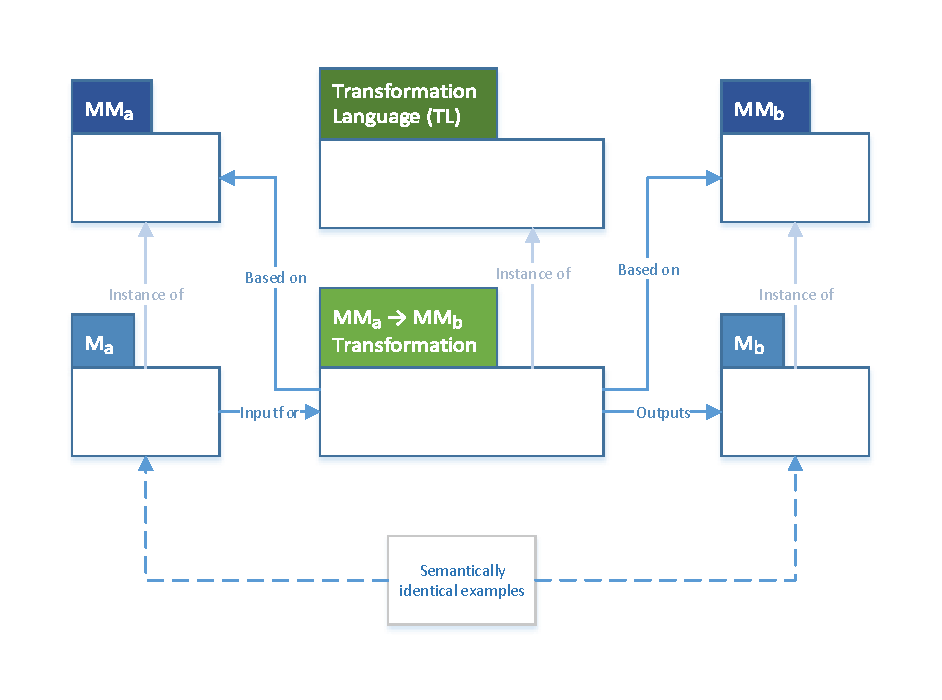
\includegraphics[scale=0.8, trim=0cm 1cm 0cm 1cm, clip=true]{Images/ProblemDomainOverview.pdf} 
	\caption{Problem domain overview - a ``MM$_a$ $\rightarrow$ MM$_b$ Transformation" has to be generated by using semantically identical input/output pairs}
	\label{figProblemDomainOverview}
\end{figure}

According to the general \gls{ModelTransformationByExample} methodology, there are two \glspl{MetaModel} MM$_a$ and MM$_b$. The task of the algorithm is to transform instances of the former into instances of the latter by performing a ``MM$_a$ $\rightarrow$ MM$_b$ Transformation". This transformation needs not be defined explicitly depending on the definition of \gls{ModelTransformationByExample}. In order to guide the algorithm, it must be able to rate a \gls{CandidateSolution}. Hence, one or more instances M$_a$ of MM$_a$ with their expected output M$_b$ conforming to MM$_b$ have to be provided. Also more information can be added as a guidance, depending on the used \gls{ModelTransformationByExample} definition. For example, details about the mapping from M$_a$ to M$_b$. This high level problem statement is refined in this chapter by answering the following questions:

\begin{itemize}
	\item What is state-of-the-art in \gls{ModelTransformationByExample}? What is the definition of \gls{ModelTransformationByExample} used in this thesis (see section \ref{secRelatedWork})? 
	\item What is a \gls{ModelToModelTransformation} given the chosen definition of \gls{ModelTransformationByExample} (see section \ref{secModelToModelTransformations})? 
	\item What renders \glspl{ModelToModelTransformation} simple or complex? What is a simple starting point for the algorithm design and development? How could the complexity be increased (see section \ref{secModelToModelTransformations})? 
	\item What are the characteristics of meta-heuristic optimization algorithms from the field of \glspl{SwarmIntelligentAlgorithm} and \glspl{EvolutionaryAlgorithm} (see section \ref{secAlgorithms})? 
	\item How can the algorithms be mapped to \gls{ModelTransformationByExample} (see section \ref{secAlgorithms})? 
\end{itemize}

%2.1 Related Work
%In order to automatically generate such ``MM$_a$ $\rightarrow$ MM$_b$ Transformations" it is at first necessary to define a more concrete goal. The first section \ref{secRelatedWork} provides an insight into existing approaches in the field of \gls{ModelTransformationByExample}. It points out the open research issues and highlights the ones that are the focus of this thesis. 

%2.2 Model-to-Model Transformations
%Transformations can have infinite different variations, which makes it difficult to find a starting point when automating those. Section \ref{secModelToModelTransformations} is therefore focusing on the identification of \glspl{ModelToModelTransformation} building-blocks.

%Therefore, at first an overview of existing \glspl{TransformationLanguage} and tools is being provided in in \ref{secExistingModelTransformationLanguagesAndTools}. Ensuring a systematic approach the idea is to identify and\/ or create definitions of a \gls{Model} and a \gls{ModelToModelTransformation} in \ref{secModelToModelTransformations} which will serve as a guideline in the universe of possible transformations. With these CMMTP at hand two kinds of examples, one for each \gls{Model} type structural and behavioral, should be created in the next chapter \ref{chapM2MScenarios} to show the actual application relevance of those for the MDD domain and at the same time provide MM$_a$ and MM$_b$ \glspl{Model} which are required to drive the prototype realization. 

%2.3 Algorithms
%In order to be able to automate \glspl{ModelToModelTransformation} a set of possible meta-heuristic optimization algorithms from the field of \glspl{SwarmIntelligentAlgorithm} and \glspl{EvolutionaryAlgorithm} are presented in section \ref{secAlgorithms}. %Those are being considered when deciding for the solution approach.

%2.4 Basic Alogrithmic Solution Approach
%Using all this information, a first draft of the algorithmic approach is being defined in section \ref{secAlgorithmicApproach}. 

%While this will already be a sound foundation it is not enough to follow the desired iterative approach yet. Therefore, an extensible example is required which will have a simple initial setup and can be extended towards a more complicated one. To define what is actually ``simple" and ``complex" a rough idea of the algorithm is needed which will be provided in  preceded by a general conceptual overview of the underlying techniques in \ref{secAlgorithms}. 

%As pointed out in \ref{figProblemDomainOverview} the ``MM$_a$ $\rightarrow$ MM$_b$ Transformation" is based on a TL which therefore must be used by the algorithm to create valid transformations. Since it is the idea to have a working prototype it is necessary to execute the generated transformations. However it is not the goal of this thesis to design and implement a \gls{TransformationExecuter} and therefore an existing language and engine have to be used.

\section{Related Work in Model Transformation By Example}\label{secRelatedWork}

The general idea of creating transformations based on given examples exists for over thirty years. Zloff was possibly one of the first who used this concept to automatically create database queries based on given example results \cite{Zloof1977}. Kohlbecker and Wand \cite{Island1987} used it to extend the functionality of Lisp-like languages and Krishnamurthi et al. \cite{Krishnamurthi2000} applied it to create XML transformations.

%programming by-example for demonstrating actions which are recorded as re-playable macros [29] Lieberman, H.: Your wish is my command: programming by example. Morgan Kaufmann Publishers Inc. (2001).

Kappel et al. \cite{Kappel2012} provided a survey which gives an overview of the current research. This is used as a guideline, extended by additional findings.

\subsection{Research Development}

%abstract vs. concrete syntax => ...

The general concept is to hide the complexity of the actual transformation from the developer of a transformation as much as possible (\cite{Zloof1977}, \cite{Island1987}, \cite{Krishnamurthi2000}, \cite{Kappel2012}). This is achieved by using manually created examples for the desired in- and/or output \glspl{Model} (M$_a$ and/or M$_b$), instead of defining a generic transformation based on the complex MM$_a$ and MM$_b$ \glspl{MetaModel}. The early approaches targeted only specific languages, but nowadays those are generic. Those approaches are not based on a specific language for MM$_a$ and MM$_b$, but uses the widely accepted \gls{MetaObjectFacility} \cite{ObjectManagementGroup2013}. This is the foundation of the \gls{UnifiedModelingLanguage} \cite{umlInfra}. 

Most of the current approaches are generating graph transformation rules or code conforming to the \gls{AtlasTransformationLanguage} \cite{Kappel2012}. \Gls{AtlasTransformationLanguage} is a textual \gls{TransformationLanguage} developed for the Object Management Group \gls{MetaObjectFacility}/QVT request for proposal (RFP) \cite{EclipseFoundation2013}. However, they may internally rely on a custom \gls{TransformationLanguage} e.g. as \cite{IvanGarcia-Magarino2009} uses a self defined ``super-transformation language" which can be translated to many common ones according to the author. Graph transformation rules are also not always directly executable and have to be converted manually \cite{Varro2007}.

Kappel \cite{Kappel2012} separated the research field in two directions based on the approaches he analyzed. However, an approach, which was not mentioned by him, requires a third one. The first direction is correspondence-based while the second one is demonstration-based, also called Model Transformation by Demonstration (MTBD). The third one is called ``chunk-based" within this thesis. Apart from that there is also another dimension which is not specific to \gls{ModelTransformationByExample} but categorizes the transformation type. The transformation might be either between instances of the same \gls{MetaModel} or between different ones. The first one is called \gls{Endogenous} while the latter is \gls{Exogenous}. This is a fundamental difference which has also implications for the \gls{ModelTransformationByExample} approaches. 

\subsection{Correspondence-based}
Correspondence-based approaches require the user to provide links between the \glspl{Object} in the examples which are usually called \glspl{Trace} (\cite{Faunes2013}, \cite{Kappel2012}, \cite{Kessentini2010a}, \cite{Kessentini2010}, \cite{Wimmer2006}). Using those a general mapping is derived.
All approaches so far have been applied to \gls{Exogenous} transformations only \cite{Kappel2012}. Since they are based on semantic correspondences, an \gls{Endogenous} transformation is probably more difficult. Such a transformation only modifies the input, hence parts of the input may remain unchanged. Possible transformations are to add, change or remove parts of the input. Correspondences in the form of ``a is transformed into b" maybe described as ``a is removed and b is added". But parts may be added without a corresponding removal as well. Hence, an application of a correspondence-based approach is at least not straight forward.

The two researchers who seem to be the drivers in this field are Wimmer and Varr\'{o}. Both are proposing a semi-automatic approach (\cite{Wimmer2006},\cite{Varro2007}) where the user has to provide the examples including the \glspl{Trace}, but later also has to fill in the gaps which could not be automatically generated or to refine the transformation.

Nevertheless, there are also differences: First Varr\'{o} creates graph \glspl{TransformationRule} while Wimmer is generating \gls{AtlasTransformationLanguage} rules. Second, the approach of Wimmer uses an algorithm which nearly creates the \glspl{TransformationRule} only directly out of the given user data. Varr\'{o} on the other hand is relying on inductive logic programming and thereby tries to derive new general concepts out of the given examples.

The two major drawbacks are related to the general idea of associating \glspl{Object} of M$_a$ and M$_b$. On the one hand \gls{Property} calculations cannot be solved well (\cite{Kessentini2010a}, \cite{Kappel2012}), probably because the user does not provide any details by definition on how to map those. On the other hand the relations are one-to-one and one-to-many on the \gls{MetaModel} level (\cite{IvanGarcia-Magarino2009}). The remaining question is, how to generate transformations for many-to-many and many-to-one relations on the \gls{MetaModel} level and many-to-many, many-to-one and one-to-many on the \gls{Model} level.

Recently, a new approach has been introduced by Faunes et al. \cite{Faunes2013} who are using an evolutionary technique. Their starting point is that they are avoiding \glspl{Trace}, because of the assumption that it is difficult to provide those for complex scenarios. Without having traces, the construction of the transformation is only based on the two given examples and no relation information. The idea is to use an \gls{EvolutionaryAlgorithm}, where each instance of the \gls{Population} is a transformation. Their quality can be evaluated by executing those with the given M$_a$ and validating to which extend it produces the expected M$_b$. Even though this is probably the most challenging approach, it is also a promising one, because it reduces the required input from the domain expert. 

However, according to the authors their approach does not work in complex scenarios, where the \gls{SearchSpace} grows fast and no solution can be found in a reasonable time. Another weakness is the assumption that semantically equivalent \glspl{Object} of M$_a$ have the same name as the ones in M$_b$ which is in fact an implicit link. Also the calculation of \glspl{Property} is not yet considered. 

\subsection{Demonstration-based}

The fundamental idea of MTBD is that the user manually transforms a self created example and all his actions are recorded. Finally, a generic transformation is distilled out of these demonstrations. This consists of a precondition for the transformation and the actual operations that have to be performed.
According to Sun et al. \cite{Sun2009}, who were the first to propose this idea, a reason for going into this new direction was that correspondence-based approaches failed to derive \glspl{Property} properly automatically. This problem is solved with MTBD easier because the user is actually performing the complex \gls{Property} calculations. Therefore it is easier to distill the generic operations. The great advantage is that the user does not only provide information about the relation of the \glspl{Object}, but also about how the \glspl{Property} are related in detail. Therefore, the algorithm has more information to create a generic transformation also for \glspl{Property}.

A major downside of MTBD is that the user must demonstrate a lot by definition which results in a high manual effort (\cite{Kessentini2010a}). Additionally, there is currently only one approach which tried to apply MTBD to \gls{Exogenous} transformations. All others are only using \gls{Endogenous} transformations \cite{Kappel2012}. It is probably easier to track changes when monitoring re-factoring. It is basically making changes to a given \gls{Model}. Whereas in an \gls{Exogenous} transformation all parts of the \gls{Model} have to be transformed into a syntactically completely different \gls{Model}.

\subsection{Chunk-based}

The assumption behind the chunk based approach is that companies often have partial transformations from previous projects. Furthermore, the goal needs not to be a generic transformation in a \gls{TransformationLanguage}, but a transformation which provides a correct M$_b$ for a given M$_a$ ``ad-hoc". The approach has been formulated by Kessentini et al. \cite{Kessentini2010} for \gls{Exogenous} transformations due to the limitations of the correspondence-based approaches.

Their idea is that there are many partial transformations which could be separated into small blocks. For a given M$_a$, the solution is a combination of blocks which completely cover the elements in M$_a$. As there are many possible combinations, \gls{ParticleSwarmOptimization} is used to search this vast \gls{SearchSpace}.

However, this approach heavily relies on the existing transformations and therefore is most likely only applicable in special situations.

\subsection{Conclusions}
\label{secRelatedWorkConclusions}

Identifying relevant approaches and their open issues requires at first a comparison of their goals with the ones of this thesis.

As a \gls{ModelDrivenDevelopment} task, which is the motivation for this thesis mentioned in section \ref{chapIntroduction}, usually transforms a \gls{PlatformIndependentModel} into a \gls{PlatformSpecificModel} an \gls{Exogenous} transformation is necessary in this context which excludes demonstration-based approaches. Even if those would not be limited to \gls{Endogenous} transformations, they generally seem to hand over a lot of work to the domain expert. This will probably not work for huge and complex transformations. So an approach with less manual effort would be desirable.

Out of the remaining two directions the chunk-based approach is also being excluded. Because it does not create a generic transformation but an ``ad-hoc" transformation thereby relying on existing transformations. This is at least a questionable assumption in general and is probably only applicable in niches.

Therefore, only correspondence-based approaches are left over.

As already mentioned most of the existing approaches are suffering from only having one-to-one links between \glspl{Object} and try to more or less directly distill the transformations based on this information. This does at least currently not work for the transformation of \glspl{Property} and more complex scenarios, which is probably an inherent problem of the focus on the links. % Consequently the complexity for the user probably exceeds his supposed low competence regarding \glspl{ModelToModelTransformation}.

Consequently, the assumption of having manually, explicitly provided links is not used within this thesis. However, this renders the achievement of a quick success even for simple examples more difficult. The approach using evolutionary techniques thereby points in a promising direction which, among \glspl{SwarmIntelligentAlgorithm}, is considered within the solution approach. As pointed out by Faunes et al. \cite{Faunes2013}, the major issue is the termination with a valid solution, since the \gls{SearchSpace} grows fast. Also, the assumption that semantically identical \glspl{Object} have the same name does probably not hold for all complex examples. Calculated \glspl{Property} are an unknown quantity as well as complex conditions. Those aspects make the \gls{SearchSpace} even larger and finding a solution more difficult.

\textbf{Definition of Model Transformation By Example}: According to the presented conclusions, the chosen definition of \gls{ModelTransformationByExample} within this thesis is as follows: A domain expert has to provide the two \glspl{MetaModel} MM$_a$ and MM$_b$. Additionally, one or more instances M$_a$ of MM$_a$ with their expected output M$_b$ conforming to MM$_b$ have to be created manually. The task of the algorithm is to create a ``MM$_a$ $\rightarrow$ MM$_b$ Transformation". Thereby, no existing transformation chunks are used which requires the creation of a transformation from scratch. Since this is a definition which relies on little information as a guidance for the algorithm, the \gls{SearchSpace} grows fast. Hence, this thesis focuses on handling large \glspl{SearchSpace} and the termination of the algorithm with a solution.

\section{Model-to-Model Transformations}\label{secModelToModelTransformations}

%pattern are on the M$_a$-M$_b$ relation level, not MM$_a$-MM$_b$ !
%pattern vs. characteristic?

As mentioned in the previous section a \gls{ModelToModelTransformation} has different challenges depending on the given transformation scenario, which has a huge impact on the complexity of the transformation. Therefore, the primary aspect covered in this section is the identification of building blocks, which could be assembled to scenarios with different complexity levels.

In order to find those blocks, the starting point is the specification of \glspl{ModelToModelTransformation}. In general, the task of a transformation is to create \glspl{Object}, associate them and assign \gls{Object} \gls{Property} values, which overall forms the output M$_b$. The challenging part is to achieve this based on a given input M$_a$, since there are infinite ways to achieve this goal. Hence, usually \glspl{DomainSpecificLanguage} are used to guide the developer and thereby restrict the possibilities to manage the complexity.

%Ensuring a systematic development approach which starts with a simple example and is extended towards a more complex one, this section is going to identify the foundations of \glspl{ModelToModelTransformation}. On behalf of those on the one hand the assembly of reference transformations scenarios with different complexity levels could be supported. On the other hand it serves as a foundation for the algorithm and prototype design.

There is no generic, common \gls{ModelToModelTransformation} language. Instead, there are a lot of different \glspl{TransformationLanguage} with different capabilities. Thus, it is not possible to refer to a common definition and use that. Rather it is necessary to analyze existing languages. One of those could be selected or an own language definition might be created for this thesis. 

Therefore, sub-section \ref{secExistingModelTransformationLanguagesAndTools} presents at first the different kinds of languages that are applicable in general considering \gls{ModelDrivenDevelopment} tasks. This section provides an overview of state-of-the art \glspl{TransformationLanguage} and corresponding tools. Since the goal is the automatic creation of \glspl{ModelToModelTransformation}, the languages are also analyzed regarding their automation potentials and obstacles.

Besides the \gls{TransformationLanguage}, the language of the \glspl{Model} M$_a$, M$_b$ and of the \glspl{MetaModel} MM$_a$, MM$_b$ has to be defined. In contrast to the first language there is a widely used and accepted \gls{ModelingLanguage}, which is presented in a simplified version.

Having an overview of existing \glspl{TransformationLanguage} and a definition of what a \gls{MetaModel} and \gls{Model} is, the last subsection \ref{secTransformationComplexity} analyzes the creation of the required simple and complex example \glspl{MetaModel} MM$_a$ and MM$_b$. The major challenge is to identify \glspl{Property} of transformations, which can be related to different complexity levels. Thus, having a foundation to create the examples as systematically as possible.

\subsection{Model-to-Model Transformation Languages and Tools}\label{secExistingModelTransformationLanguagesAndTools}

A \gls{ModelToModelTransformation} can be implemented via any general purpose language, because it is basically a program that gets a \gls{Model} M$_a$ as an input and creates a \gls{Model} M$_b$ as an output. Hence, the transformation itself is not restricted through the general definition. Since an automation is not possible without any underlying specification, a \gls{DomainSpecificLanguage} for \glspl{ModelToModelTransformation} is required. This language restricts the possibilities and thereby defines what a transformation actually is in the context of the thesis. %Otherwise many programs would be created which do something, but not the intended \gls{ModelToModelTransformation}.

There are two options to get such a \gls{DomainSpecificLanguage}: either creating one or using an existing one. Besides defining a \gls{DomainSpecificLanguage}, a \gls{TransformationExecuter} might have to be created, which is required to perform the transformation. Overall, there are four general possible categories from creating everything from scratch to relying completely on existing solutions.

Additionally, a hybrid approach is possible: An example is presented by \cite{Faunes2013}, who used a self-created \gls{DomainSpecificLanguage} for the automatic generation, which is then translated into an existing rule language. This result is being executed by an existing rule engine. %A rule language basically consist of ``IF-THEN" patterns and is usually used to compute business rules.

Starting with a self-defined language might be easier, because it can be tailored for the given scenario and therefore kept small. This advantage might turn into the opposite when introducing other, more complex scenarios. Then, it is likely that the language definition contains limitations. They can result in extensive refactoring not only of the language itself, but also of the \gls{TransformationGenerator} and \gls{TransformationExecuter}. In contrary, existing languages, which have proven their usefulness in many cases, have a lot of language constructs which are not required for the first scenarios, but are not facing the risk of being unable to solve more complex tasks. 

Therefore, existing languages are analyzed at first. A systematic language selection requires the specification of the transformation tasks to be solved. In \cite{Mens2006} a taxonomy for \glspl{ModelToModelTransformation} is provided which serves as a blueprint for the language requirement definition. 
The type of source and target elements has to be specified. They are either programs or - in this case - \glspl{Model}. 
Furthermore, a transformation might use several in- and/or output \glspl{Model}. In \gls{ModelDrivenDevelopment} the most common task is transforming a single \gls{PlatformIndependentModel} into a single \gls{PlatformSpecificModel} and therefore only one \gls{Model} is required.

Apart from that, there is also the previously explained distinction of transformations between instances of the same \gls{MetaModel} and different ones. The first one is called \gls{Endogenous} while the latter is \gls{Exogenous}. As already described in section \ref{secRelatedWork}, an \gls{ModelDrivenDevelopment} task usually transforms a \gls{PlatformIndependentModel} into a \gls{PlatformSpecificModel}. Hence, an \gls{Exogenous} transformation is necessary.

Additionally, a transformation may be horizontal when both in- and output \gls{Model} are on the same abstraction level or vertical otherwise. As the \gls{ModelDrivenDevelopment} transformations are between \glspl{Model} of different types but at the same level, a horizontal transformation is performed. An example is the \gls{RelationalSchema}. It is still on the same abstraction level as the originating \gls{ClassDiagram}, but conforms to a specific platform.

Finally, there is a distinction between syntactical and semantical transformations. In the domain of \gls{ModelTransformationByExample} the idea is to have two semantically identical \glspl{Model} created by a domain expert. Therefore, the transformation is only syntactical. %It must be pointed out that \gls{ModelDrivenDevelopment} transformations may also make syntactical changes and therefore using \gls{ModelTransformationByExample} restricts the possibilities in terms of \gls{ModelDrivenDevelopment}.

Summarizing all properties a horizontal, \gls{Exogenous} \gls{TransformationLanguage} using one in- and output \gls{Model} for syntactical transformations is required.

On top of the fundamental constraints, there are also requirements derived from the first insights into \glspl{EvolutionaryAlgorithm} and \glspl{SwarmIntelligentAlgorithm}. The priority list defines the importance, starting with the most relevant.

\begin{itemize}
\item Language Requirements
	\begin{itemize}
	\item language capabilities should be state of the art and proven in the field, to minimize language based restrictions when designing the representative \glspl{ModelToModelTransformation} scenarios
	\item a detailed specification of the language is required to avoid manual reverse engineering	
	\item \glspl{TransformationRule} and constructs should be independent to allow an easy modification without considering the context	
	\item it should allow a ``simple start" - meaning that a basic transformation should not involve too many constructs that have to be identified by the algorithm	
	\end{itemize}

\item Tooling Requirements
	\begin{itemize}
	\item a \gls{TransformationExecuter} must exist for the language as it is not the scope of this thesis to design and implement the actual transformation execution
	\item the \gls{TransformationExecuter} must support ``stand-alone" execution, i.e. it must not be bound to a graphical user interface exclusively which prohibits automatic execution
	\item the \gls{TransformationExecuter} should have a high performance which might increase the possibility to find the right transformation in an \gls{EvolutionaryAlgorithm} or \gls{ParticleSwarmOptimization} algorithm
	\item a visual representation of transformation \glspl{Trace} is desired to simplify the analysis and comparison of the results during the prototype test phase
	\item an active community should be present which can assist in solving technical issues
	\end{itemize}
\end{itemize}

%It must be pointed out that these are basic criteria regarding a language selection. When it comes to complicated transformations much more details have to be analyzed as conducted by Sven and Lars Patzina \cite{Patzina}. Nevertheless for the general selection of a language it should be sufficient as long as the language has proven to be useful for common transformation challenges in the field.

Having these criteria defined, the relevant subset of languages consists of three fundamentally different types. The first one is textual \glspl{DomainSpecificLanguage} for \glspl{ModelToModelTransformation}, the second one is graph transformation based \glspl{DomainSpecificLanguage} for \glspl{ModelToModelTransformation} and the third one is logical programming. 

Textual \glspl{DomainSpecificLanguage} are subdivided based on the used mechanisms into declarative, operational and logic programming approaches according to \cite{Mens2006}. According to the comparison of Mens et al., the declarative approaches have a lot of implicit behavior compared to operational ones. This results in an easier language with less explicit dependencies but at the same time it restricts also the capabilities i.e. when the execution order is relevant or when there is no direct relationship \cite{Dvorak2008a}. For logical languages no direct comparison towards the other two types is being provided.

Graph transformation based \glspl{DomainSpecificLanguage} are divided into purely declarative languages and hybrid languages which allow operational constructs to e.g. define the execution order and avoid an implicit and non-deterministic execution order \cite{Detten2012}. 
%TGGs are similar to declarative approaches especially regarding the implicit and non-deterministic execution order \cite{Detten2012}. The SDM approach is similar to the operational one since it uses UML Activity Diagrams \cite{umlInfra} to define the transformation order.
%triple graph grammars (TGG), story driven modeling (SDM)

Logical programming is divided into forward and backward chaining languages. The former is the more intuitive one, because it is in the form of if-then-else statements while the latter one is based on deduction.

The following languages and \glspl{TransformationExecuter} have been identified as candidates for this thesis. Overall there had been about thirty within scope at first, but most of them either did not fit the general properties defined above at all or seemed to be discontinued.

\begin{itemize}
\item Textual \glspl{DomainSpecificLanguage} for \glspl{ModelToModelTransformation}
	\begin{itemize}
	\item Declarative:
			\begin{itemize}
			\item QVT-Relations (\cite{ObjectManagementGroup2011}): Eclipse Modeling Project (\cite{EclipseFoundation2014a})
			\item \gls{AtlasTransformationLanguage}: Eclipse Modeling Project (\cite{EclipseFoundation2013})
			\item jQVT: JQVT (\cite{Song2012})
			\item \gls{EpsilonTransformationLanguage}: Eclipse Epsilon (\cite{Kolovos2013}, \cite{EclipseFoundation2012})
			\end{itemize}
	\item Operational: 
		\begin{itemize}		
		\item QVT-Operational: Eclipse Modeling Project (\cite{EclipseFoundation2014a}), Magic Draw (\cite{NoMagicInc})
		\end{itemize}
	\end{itemize}
	
\item Graph transformation (Triple Graph Grammar) based \glspl{DomainSpecificLanguage} for \glspl{ModelToModelTransformation}
	\begin{itemize}
	\item Declarative: TGG (\cite{Greenyer2014}), eMoflon (\cite{Real-TimeSystemsLab2014}), MoTE (\cite{Hildebrandt})%, Groove (ref TODO) % focues on verification...
	\item Hybrid (Declarative \& operational): eMoflon, MoTE, Henshin (\cite{EclipseFoundation2013a})%, EMorF (ref TODO)
	\end{itemize}


\item Logical Programming:
	\begin{itemize}		
	\item Forward chaining %RETE! = Rule Engines
		\begin{itemize}
		\item JESS: JESS (\cite{SandiaNationalLaboratories2013}) %http://jess.2305737.n4.nabble.com/JESS-equivalent-rule-of-a-prolog-rule-td3958608.html
		\end{itemize}
	\item Backward chaining
		\begin{itemize}
		\item Prolog: GNU Prolog (\cite{Diaz2013}), SWI-Prolog (\cite{Wielemaker2013})%, C\#Prolog (\cite{Pool2014})
		\end{itemize}
	\item Both
		\begin{itemize}
		\item Drules: JBoss Drools (\cite{RedHat2014})%, Drules.NET (ref TODO) %http://programmers.stackexchange.com/questions/114711/the-relation-between-business-rules-engines-and-constraint-programming-languages
		\end{itemize}
	\end{itemize}

\end{itemize}	

After this rough overview of the different language types and a pre-selection of possible languages the next step is to get a deeper insight into the concepts of \glspl{TransformationLanguage}. Those are compared against the requirements to select the most appropriate language. 

The ones in the logical programming category have been excluded from a further investigation. Since those languages provide no specific constraints and guidelines for \glspl{ModelToModelTransformation}, their application in this context would not provide the desired foundation. Hence the first two are considered to distill the essential ideas of \glspl{ModelToModelTransformation}.

The characteristic aspects of those two language categories are now presented in a survey-like manner to point out the basic concepts, commonalities and differences. %Not every language is presented because the focus is on the general concepts, not the syntactic details of every language.

\textbf{Textual languages} \Gls{AtlasTransformationLanguage} is currently a popular and widely used language in that category (\cite{IvanGarcia-Magarino2009}). It has a large set of features and has therefore been chosen as the primary example language. Listing \ref{lstATLExample} shows an instance of a \gls{AtlasTransformationLanguage} transformation that makes use of key features which have been extracted from \cite{INRIA2005}. 

At first, it is important to note that ``modules" containing ``rules" have to be defined in \gls{AtlasTransformationLanguage}. The former defines MM$_a$ and MM$_b$ and the latter defines mappings for each \gls{Class} of MM$_a$ to a MM$_b$ \gls{Class}. As \gls{AtlasTransformationLanguage} follows the relational approach, there is no order defined in which the \glspl{TransformationRule} have to be applied. Instead, each \gls{TransformationRule} has a ``from" condition which defines for which \glspl{Class} this \gls{TransformationRule} can be applied. A restriction of \gls{AtlasTransformationLanguage} is that a \gls{TransformationRule} must be unique, meaning that every \gls{Object} in M$_a$ can only be matched by one \gls{TransformationRule}.

Nevertheless, also the ``to" condition may constrain the \glspl{TransformationRule} application as it may refer to previously mapped \glspl{Object}. This has been used in line 50 where ``resolveTemp" refers to the output of the ``\Gls{Class}2Table" \glspl{TransformationRule} named ``key". Hence an order is defined implicitly.

Besides, the mappings in general \gls{AtlasTransformationLanguage} allows the definition of conditions or aggregations e.g. in line 20 and 44 with the \gls{ObjectConstraintLanguage}.

So-called helpers are another type of construct, seen in line 31. Those may encapsulate complex aggregations and provide a possibility to reuse those in many different places.

\begin{lstlisting}[language=ATL,caption={\Gls{AtlasTransformationLanguage} example},label={lstATLExample}]
-- The prerequisite for this mapping is a
-- MMa called 'ClassModel' and a MMb called 'EntityRelationshipModel'
-- The further contains Classes with Properties while
-- the latter contains Tables with Columns.
module ClassModel2EntityRelationshipModel;
create OUT : EntityRelationshipModel from IN : ClassModel; 

-- Create a table for each Class.
-- The table has the same name as the Class
-- and the columns of the table contain the 'key' 
-- which did not exist in the Class. All other 
-- columns are mapped in 'Property2Column' but are 
-- also included in the 'columns' list of the table.
rule Class2Table {
	from
		c : ClassModel!Class
	to
		table : EntityRelationshipModel!Table (
			name 	<- c.name,
			columns <- Sequence {key}
					->union(c.attr->select(e | not e.multiValued)),
		),
		key : EntityRelationshipModel!Column (
			name <- 'Id',
			type <- thisModule.objectIdType
		)
} 

-- The type of a 'key' created in Class2Table is defined ad hoc in
-- the rule with the following helper
helper def : objectIdType : EntityRelationshipModel!Type =
	ClassModel!DataType.allInstances()
		->select(e | e.name = 'Integer')->first(); 

-- Create a column in a table for each Property in a Class.
-- Use only Properties which have have simple types
-- and are no reference to another Class.
-- The column has the same name and type as the Property
-- but has additionally the owner set to the table corresponding
-- to the Class of the Property.
rule Property2Column {
	from
		a : ClassModel!Property (
			a.type.oclIsKindOf(Class!DataType) and not a.multiValued
		)
	to
		out : EntityRelationshipModel!Column (
			name <- a.name,
			type <- a.type,
			owner <- thisModule.resolveTemp(a.owner, 'key')
		)
} 
\end{lstlisting}			

Overall, \gls{AtlasTransformationLanguage} consists of about 90 \glspl{ProductionRule} (see \cite{EclipseFoundation2013}) which shows that there are a lot more aspects covered that have not been explained here, because the focus is on the general concepts.

In contrast, QVT-Operational does - as the name indicates - not follow the relational approach and therefore allows the definition of a \gls{TransformationRule} execution order. Listing \ref{lstQVToExample} which has been extracted from \cite{Rubby2012} shows this kind of definition in line 5 and 6.

\begin{lstlisting}[language=QVT,caption={QVT Operational example},label={lstQVToExample}]

main() {
	srcModel.objectsOfType(Class)->map Class2table();
	srcModel.objectsOfType(Association)->map Association2table(); 
}
	
mapping Class::Class2table () : Table
	-- ...
} 
	
mapping Property::Property2column(): Column {
	-- ...
} 	
\end{lstlisting}

It has to be pointed out that when executing instances of relational languages there can be situations where multiple \glspl{TransformationRule} are applicable. Therefore, it depends on the \gls{TransformationExecuter} which one is chosen. This kind of unpredictability, respectively \gls{TransformationExecuter} specific behavior, is avoided in operational languages by handing this task over to the user of the language.

QVT-Operational has also a more fine-grained concept \cite{ObjectManagementGroup2011} for referring to mappings of \glspl{Object} which was covered by ``resolveTemp" in \gls{AtlasTransformationLanguage}. First, it is possible to get the M$_b$ element for a given M$_a$ element with ``resolve()" or even vice-versa with ``resolvein". In addition to that, one can specify that a resolve should be performed deferred with ``late resolve()". This is useful when the specified \gls{TransformationRule} execution order maps the \gls{Object} that should be resolved, after the current rule.

\textbf{Graph \glspl{TransformationLanguage}} 

This type of \gls{TransformationLanguage} uses a different approach, as the first impression of an example in Henshin \cite{EclipseFoundation2013a} shows (see figure \ref{figHenshinExample}).

The transformation is also part of a ``\Gls{Class}2Table" \gls{TransformationRule} set as the previous ones. The figure shows one \gls{TransformationRule} which is defined in a box having the \gls{ClassDiagram} on the left hand side and the \gls{RelationalSchema} on the right hand side. In between there are the \glspl{Trace} which actually define the relations. It has to be pointed out, that this type of definition also allows a bidirectional mapping in contrast to the textual \glspl{DomainSpecificLanguage}. Another difference is that one \gls{TransformationRule} definition actually defines many different conditional mappings defined in double angle brackets. For example ``$\langle\langle$preserve*/tab/col$\rangle\rangle$" is an instruction which is only relevant for others which are restricted to ``*/tab/col".
		
\begin{figure}[htb]
	\centering
	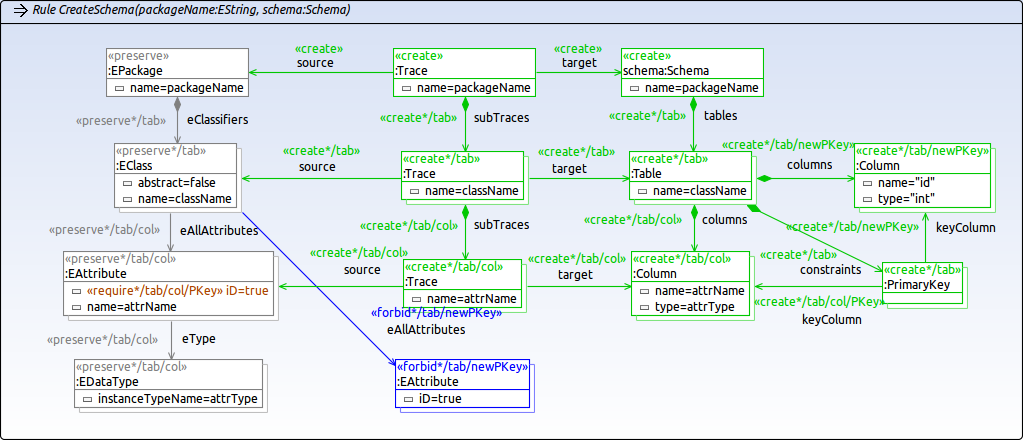
\includegraphics[scale=0.40,natwidth=1023,natheight=440]{Images/HenshinExample.png} 
	\caption{Henshin example}
	\label{figHenshinExample}
\end{figure}		

According to the developers of Henshin, the power of the underlying XML format exceeds the one of the graphical definitions and looks quite different when being compared to the visual representation. Therefore, a lot more complexity has to be expected when going deeper into this type of language.

After providing an overview of the \gls{ModelToModelTransformation} concepts found within the \glspl{DomainSpecificLanguage}, the language and tooling requirements are analyzed in the following paragraphs.

Considering the language requirements, some of them have been already fulfilled during the pre-selection. First of all, the selected languages are state of the art and have a detailed specification. The requirement of having independent \glspl{TransformationRule} and constructs is not fulfilled by operational textual \glspl{DomainSpecificLanguage} as they need an explicit \gls{TransformationRule} execution order to be defined. Finally, the ``simple start" is supported by all \gls{ModelToModelTransformation} \glspl{DomainSpecificLanguage}, because their design purpose was to provide a simple language for this domain. This excludes logical programming, since those languages are designed for more general purposes as already mentioned before.

On the other hand, the tooling requirements need to be inspected. As it is not the focus of this thesis to go deep into this matter, the explanations are short. The first requirement of providing a \gls{TransformationExecuter} was already fulfilled in the pre-selection. The second one of supporting non-user-interactive execution, i.e. providing a well documented and easy-to-use API for stand-alone execution, is  not fulfilled by any \gls{TransformationExecuter}. This is due to the fact that their primary purpose is to support a user in front of a modeling environment like Eclipse. Nevertheless, is was possible to create a ranking, in which the graph transformation engines marked the bottom line. The third requirement of providing high performance execution is not fulfilled by the \gls{AtlasTransformationLanguage} execution engine, since it is executed within its own, slow virtual machine. Providing a visual representation for \glspl{Trace} is provided by graph \glspl{TransformationExecuter}. Finally, an active community is more or less present for all of them. Especially well supported are \gls{AtlasTransformationLanguage} and the \gls{EpsilonTransformationLanguage}.

\textbf{Conclusion}: Overall, the declarative textual \glspl{DomainSpecificLanguage} in general and within this category the \gls{EpsilonTransformationLanguage} matched the requirements best compared to the others. The existing \gls{TransformationLanguage} and \glspl{TransformationExecuter} used in this thesis is the \gls{EpsilonTransformationLanguage}.

Besides selecting a \gls{TransformationLanguage} and \gls{TransformationExecuter} it is also necessary to create or select a language for the \glspl{MetaModel} themselves which is evaluated in the following sub-section.

% The most common modeling language in software engineering is the Unified Modeling Language (UML) \cite{umlInfra} and therefore it is recommendable to use it when possible.

\subsection{Meta-Model Language}\label{secModelLanguage}

To define patterns it is necessary to define the language of MM$_a$ and MM$_b$. For example, talking about a ``1:1 mapping between \glspl{Class}" assumes that there must be a \gls{Class} in both languages of MM$_a$ and MM$_b$ and also assumes that both share the same language. The refined problem domain overview in figure \ref{figProblemDomainOverviewRefined} contains this \gls{MetaMetaModel} MMM. It is on abstraction level M3 whereas the \gls{MetaModel} MM$_a$ and MM$_b$ are on level M2 and the concrete \glspl{Model} are on level M1.

\begin{figure}[htb]
	\centering
	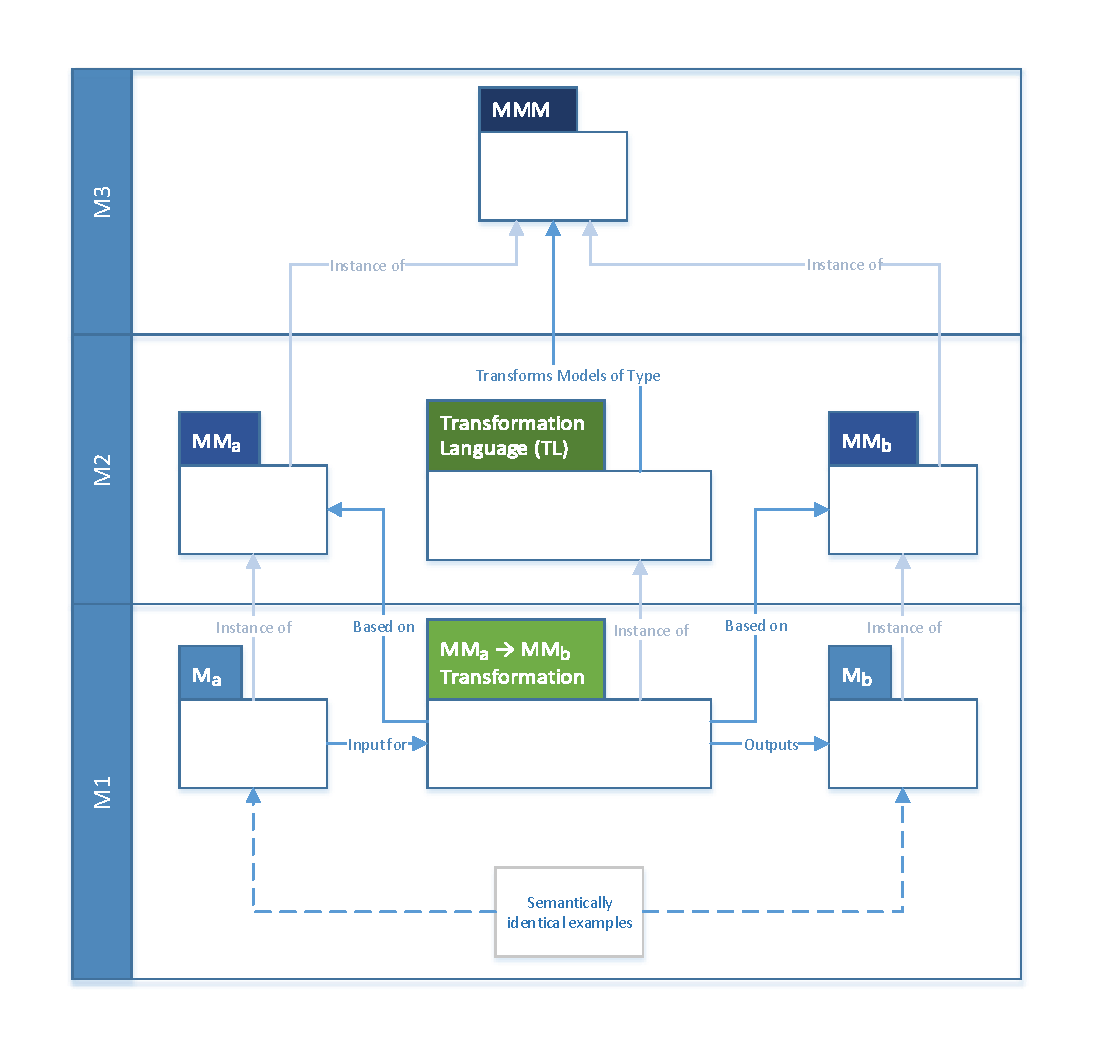
\includegraphics[scale=0.76, trim=0cm 1cm 0cm 1cm, clip=true]{Images/ProblemDomainOverviewRefined.pdf} 
	\caption{Problem domain overview refined - a ``MM$_a$ $\rightarrow$ MM$_b$ Transformation" has to be generated by using semantically identical input/output pairs. The input and output \glspl{MetaModel} MM$_a$ and MM$_b$, as well as the \gls{TransformationLanguage} conform to the meta-\gls{MetaModel} MMM.}
	\label{figProblemDomainOverviewRefined}
\end{figure}

An important distinction in the field of \glspl{ModelingLanguage} is the differentiation between the \gls{AbstractSyntax} and the \gls{ConcreteSyntax}. The \gls{AbstractSyntax} is a representation-independent language whereas the \gls{ConcreteSyntax} is a visually enhanced representation, optimized for the purpose of a specific language, with a mapping to the \gls{AbstractSyntax}. In this context, only the \gls{AbstractSyntax} is considered because it represents the generic foundation. 

As mentioned in section \ref{secRelatedWork}, the common language in \gls{SoftwareEngineering} is the \gls{UnifiedModelingLanguage} which is therefore used, among others, as a blueprint for the languages MM$_a$ and MM$_b$. In \gls{UnifiedModelingLanguage} the \gls{AbstractSyntax} can be described in the self-defining \glsfirst{MetaObjectFacility}. Hence, \gls{MetaObjectFacility} is the shared language MMM of MM$_a$ and MM$_b$ as it allows the use of \gls{UnifiedModelingLanguage} as well as other languages. 

Another method for defining languages on M2 is the light-weight extension mechanism of \gls{UnifiedModelingLanguage}, called profiles. The advantage of profiles is that everything what has been defined in \gls{UnifiedModelingLanguage} can be re-used. Since the support of profiles in the context of \glspl{ModelToModelTransformation} is not yet provided \cite{Randak2011}, this is not an option. As the thesis has the focus on automating \glspl{ModelToModelTransformation} the well supported \gls{MetaObjectFacility} is used.

As \gls{MetaObjectFacility} itself contains a large number of language constructs (\cite{ObjectManagementGroup2013}) which cover concepts that are not relevant for this thesis, it is reduced in such a way that it supports only the definition of basic structures. This is enough to specify basic languages on M2 and at the same time limits the complexity. It has to be pointed out that this is not a completely new language, but a reduced version of \gls{MetaObjectFacility} in order to avoid the undesired effects of self-defined languages described in the previous sub-section.

The illustration in Figure \ref{figMOFSimplified} shows the simplified \gls{MetaObjectFacility} definition in \gls{ConcreteSyntax} which allows the description of structures. Elements named ``\Glspl{Class}" are shown as boxes and their relations named ``\Gls{Association}" are shown as lines. 

\begin{figure}[!ht]
	\centering
	%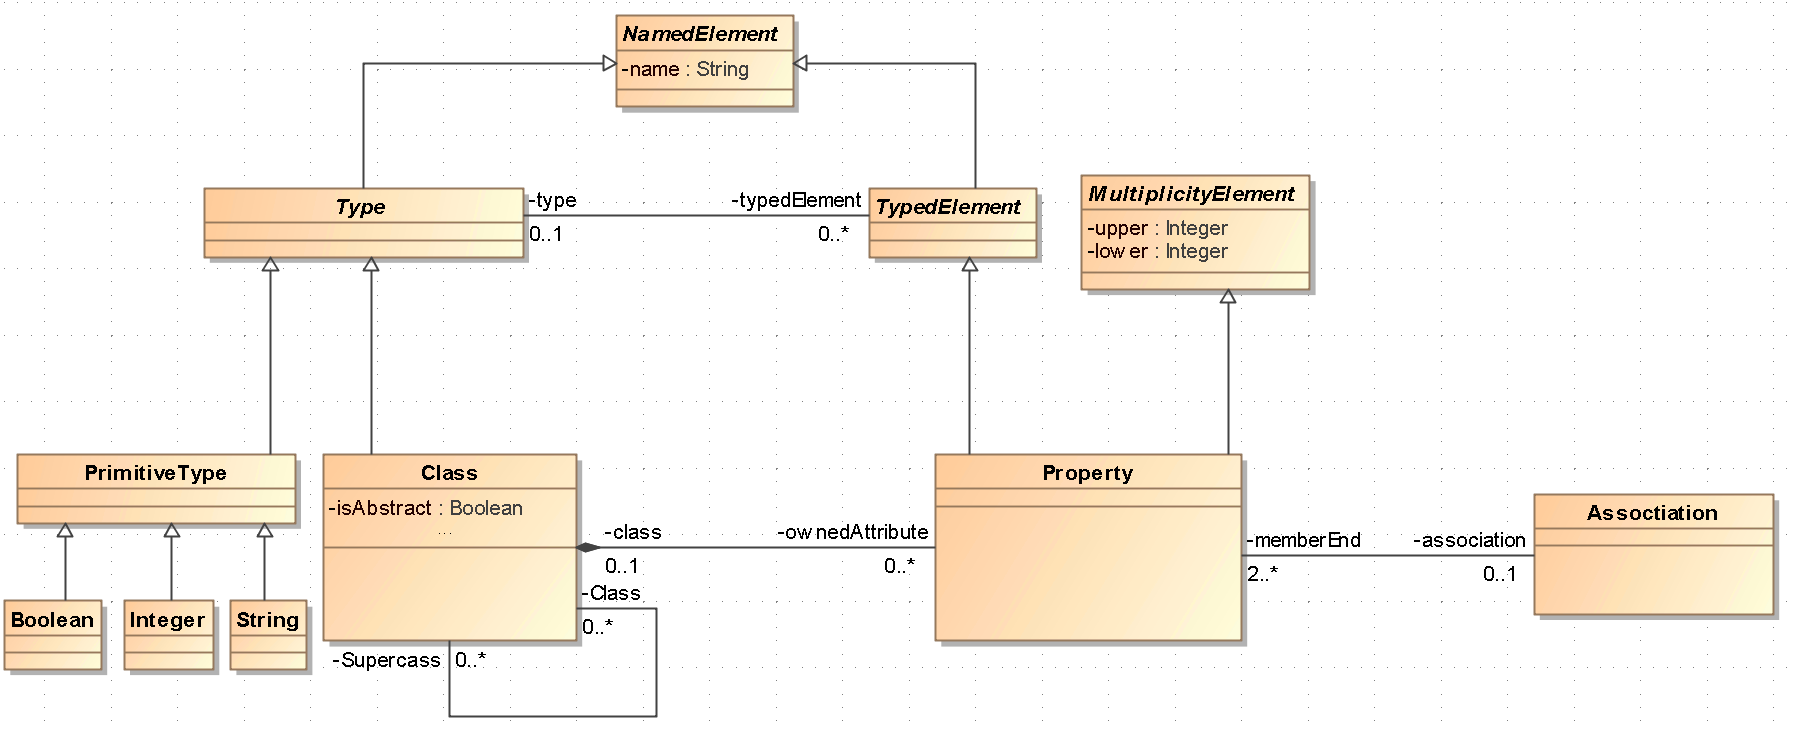
\includegraphics[scale=0.30,natwidth=1793,natheight=733]{Images/MOFSimplified.PNG} 
	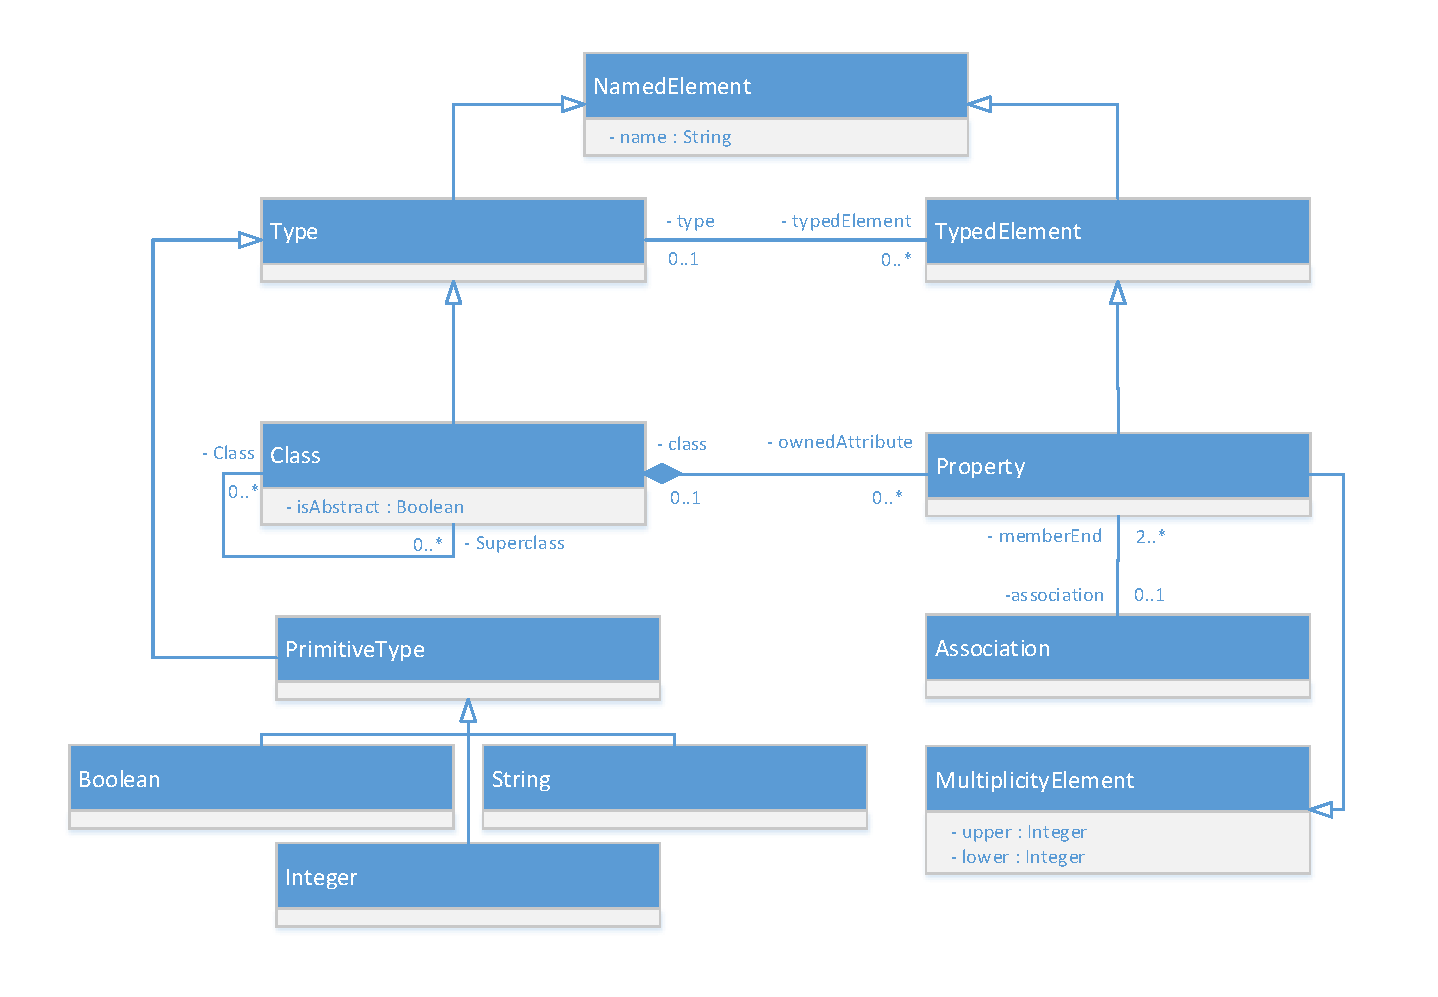
\includegraphics[scale=0.6, trim=0cm 1cm 0cm 1cm, clip=true]{Images/MOFSimplified.pdf} 
	\caption{\Gls{MetaObjectFacility} simplified}
	\label{figMOFSimplified}
\end{figure}

Additionally, ``\Glspl{Class}" consist of ``\Glspl{Property}" that may be the start or end of an ``\Gls{Association}" thereby being an ``MultiplicityElement" that describes how many of the associated ``\Glspl{Class}" are required and/or allowed i.e. ``0..1" is defined as ``lower=0" and ``upper=1" in the \gls{AbstractSyntax}. 

``\Glspl{Property}" may also be simple ``PrimitiveTypes" e.g. a ``String" or an ``Integer", or even ``\Glspl{Class}" which are visualized e.g. as ``upper: Integer" in the \gls{ConcreteSyntax} which is a \gls{Property} named ``upper" with a ``PrimitiveType". 

A \gls{Class} defines also a self-reference to describe the concept of inheritance by defining super-\glspl{Class} which derive everything to their sub-\glspl{Class}. In the \gls{ConcreteSyntax} this is visualized through lines with arrows at the end. 

``\Glspl{Class}" may also be marked as ``IsAbstract" which defines that they cannot be instantiated directly, only by deriving from it. In the simplified \gls{MetaObjectFacility} definition all ``\Glspl{Class}" with names in italic font are abstract. 

Finally almost everything must be able to get a proper name. Hence, most inherit from ``NamedElement".
%The Simplified \gls{MetaObjectFacility} definition is not completely self-describing as it uses role names for the ends of the association to improve the readability.

\gls{MetaObjectFacility} is sometimes not sufficient to describe a language, because it covers only the structural aspects without the possibility to specify i.e. constraints or calculated \glspl{Property}. Therefore, the \glsfirst{ObjectConstraintLanguage} \cite{ObjectManagementGroup2012} is defined in the \gls{UnifiedModelingLanguage}. It provides constructs to define conditions or calculated \glspl{Property}. Since those aspects would add more complexity and are not mandatory in basic languages, they are excluded to avoid unnecessary issues.

\subsection{Transformation Complexity}\label{secTransformationComplexity}

In the previous subsections an overview of \glspl{TransformationLanguage} has been presented as well as a definition of the M$_a$ and M$_b$ languages. The general approach of this thesis includes the construction of \glspl{MetaModel} for M$_a$ and M$_b$ which result in transformations ranging from simple to complex. Thus, this sub-section is focusing on the question how this construction can be performed systematically.

Up until now research does not provide such kind of systematic approach besides some indications (\cite{Strommer2007}, \cite{IvanGarcia-Magarino2009}, \cite{Patzina}). Nevertheless at least some basic categorizations regarding transformation complexity have been defined. But the perspective is usually based on the solution, the \gls{TransformationGenerator}, not the transformation.

Considering the analyzed related work (see section \ref{secRelatedWork}), an easy starting point are one-to-one \glspl{Object} transformations which do not require any pre-conditions and no \gls{Property} calculations. Both pre-conditions and \gls{Property} calculations may require complex queries, resulting in a more sophisticated \gls{TransformationGenerator}.

A further distinction was introduced by \cite{Strommer2007} between a so called ``Simple Mapping" and a ``Compound Mapping". Within the former one \gls{Class} of M$_a$ is mapped to exactly one of M$_b$. In the latter multiple \glspl{Class} of M$_a$ are mapped to multiple ones of M$_b$. Additionally, there are ``String Manipulations", which include all transformation operations, manipulating string-\glspl{Property} such as converting a character sequence to lower case before using it for a comparison. There were also some other categories which were not that generic, but rather specifically targeted at the approach. The mentioned definitions could also be found in other approaches and seem to be the unofficial standard regarding transformation complexity.

However, there are also other definitions which provide additional categories like \cite{IvanGarcia-Magarino2009} and \cite{Patzina}. The previously mentioned categories could be found here, too but also use e.g. the generation of constraints and the usage of negative examples as an input. Those categories are defined from a solution point of view. They do not directly describe what actually makes a transformation more or less complex and how to systematically evolve such a transformation.

Summarizing the existing research and merging it into the previously provided foundations is the next step. Foremost, the complexity of a transformation is related to the number and kind of relations between the \glspl{Class} on M2. For example, if a \gls{Class} of M$_a$ is always transformed into a specific \gls{Class} of M$_b$, this results in a simple 1:1 mapping. Assuming that the \gls{Class} of M$_a$ is transformed into two \glspl{Class} of M$_b$, this results in much more possible transformations, because the number of relations to be considered between \gls{Class} of M$_a$ and M$_b$ is 1:N and hence increases. Furthermore also N:1 and N:M are possible.

The same applies to the M1 level, where these kinds of relations are applicable. For example one \gls{Object} in M$_a$ can be transformed into two or more of the same type in M$_b$. This kind of transformation is usually not mentioned in the literature, but contains different challenges in the solution and should be handled separately. Considering the given example, there must be a definition especially for the number of the \glspl{Object} to be created. This can be either a value in an \gls{Object} in M$_a$ specifying the number of instances, a fixed number defined in the transformation or any kind of mathematical expression.

Besides the kind of relation, it has to be considered what could be related. Based on the definition of the simplified \gls{MetaObjectFacility} the possible relations, which can be defined in the mapping between M2 \glspl{Model}, are limited to the instances of non-abstract members of MMM in M3 which are \glspl{Class}, \glspl{Property}, \glspl{Association} and primitive types. Abstract members can be excluded because they are never directly used when creating a \gls{MetaModel} based on \gls{MetaObjectFacility} and are included in the non-abstract members via inheritance.

Basically, all of these can be related e.g. \glspl{Class} to \glspl{Class} with the defined relation possibilities like 1:N. Furthermore a transformation from a \gls{Class} to a \gls{Property} is possible, which increases the complexity. Finally a mixture can be necessary like transforming a \gls{Class} into a \gls{Property} and an \gls{Association}.


%=> define in scenarios!?
%
%c = \{c_1,c_2, ... c_n\}
%p = \{p_1,p_2, ... p_m\}
%a = \{a_1,_a2, ... a_o\}

%$$MM_\varsigma = \{ c \mid c -instanceOf-MOF Class \}$$
%$$MM_\rho = \{ p \mid p -instanceOf-MOF Property \}$$
%$$MM_\alpha = \{ a \mid a -instanceOf-MOF Association \}$$
%
%$$MM = \{c \mid c \in MM_\varsigma\} \cup \{p \mid p \in MM_\rho\} \cup \{a \mid a \in MM_\alpha\}$$
%$$MM_a,MM_b,MM_x \in MM$$
%
%$$M_\varsigma = \{ c \mid c -instanceOf-\varsigma, \varsigma \in MM_\varsigma \}$$
%$$M_\rho = \{ p \mid p -instanceOf-\rho, \rho \in MM_\rho \}$$
%$$M_\alpha = \{ a \mid a -instanceOf-\alpha, \alpha \in MM_\alpha \}$$
%
%$$M_x = \{c \mid c \in M_\varsigma\ \land c -instanceOf- MM_x\} \cup$$
%$$ \{p \mid p \in M_\rho\ \land p -instanceOf- MM_x\} \cup $$
%$$ \{a \mid a \in M_\alpha\ \land a -instanceOf- MM_x\}$$

%%%\
%%%
%%%\begin{enumerate}
%%%	\item One-to-One on M2 and M3 = $\{(a_A,b_B) \mid A \in {MM}_a, B \in {MM}_b\, a \in {M}_a, b \in {M}_b$
%%%	\item One-to-One on M2 and M3 - context sensitive = \\$\{(A,B,c) \mid A \in {MM}_a, B \in {MM}_b, c \in Constraints\}$
%%%	\item One-to-Many on M3 = $\{(A,B_1,..,B_n) \mid A \in {MM}_a, B \in {MM}_b \}$
%%%\end{enumerate}
%p -> p
%a -> a
%
%c -> p
%c -> a
%p -> c
%p -> a
%a -> c
%a -> p
%
%\\


%c|a(x) -> ...
%c|b(x) -> ...
%
%
%
%1:N - M3
%c -> c_1, c_2, c_n
%...
%
%1:N - M2
%c -> c, p
%c -> c, p, a
%...
%
%1:N - M2 + M3
%c -> c_1, c_2, p_1
%...
%
%1:N - M2 and/or M3 - context sensitive
%c|a(x) -> ...
%c|b(x) -> ...
%
%
%
%
%N:1 - M3
%...
%
%N:1 - M2
%...
%
%N:1 - M3 + M2
%...
%
%N:M - M3
%...
%
%N:M - M2
%...
%
%N:M - M2 + M3
%...
%
%...



%%%$$ \{(c_1,p_1,a_1),...,(c_n,p_m,a_o)\} X \{c,p,a\}

This idea might help to systemically develop \glspl{MetaModel} for M$_a$ and M$_b$ which result in transformations with different complexity levels. Though, it remains incomplete as in general a transformation can be more difficult e.g. when considering the computation of \glspl{Property} or pre-conditions for the application of a mapping.

\section{Meta-Heuristic Optimization Algorithms}\label{secAlgorithms}

In contrast to the most existing approaches, this thesis is trying to solve the generation of \glspl{ModelToModelTransformation} without using a direct deduction from manually provided links or recorded user transformations. Instead, the idea is to utilize meta-heuristic optimization algorithms to construct the transformation. As an input, only the manually created \glspl{Model} M$_a$ and M$_b$ are used. They are the reference for correctness of the created solution. Therefore, algorithms are required that are able to cover large \glspl{SearchSpace} because a \gls{ModelToModelTransformation} can become complex with these assumptions (see sections \ref{secRelatedWork} and \ref{secTransformationComplexity}).

The meta-heuristic optimization algorithms, that are analyzed for possible applications, are from the field of \glspl{SwarmIntelligentAlgorithm} and \glspl{EvolutionaryAlgorithm}.

The fundamental requirement to apply such algorithms is the reduction of the given problem. Every algorithm expects a certain \gls{Encoding} of the problem, with different restrictions, which is used to represent a \gls{CandidateSolution} and thereby defines the \gls{SearchSpace} (\cite{holland75},\cite{Dorigo},\cite{Cook1997}).

In general the algorithms are categorized into combinatorial and generative (\cite{holland75},\cite{Dorigo},\cite{Cook1997}). The former requires that the \gls{Encoding} of the problem consists of a finite set of building blocks that can be assembled to a solution. The algorithm either uses a discrete approach, to pick any blocks or a continuous one, i.e. weights or probabilities are assigned to the blocks. The latter category is used to create something from scratch without the need to have a finite set of building blocks.

Without having any guidance in a \gls{SearchSpace} each algorithm would perform a random search. Hence, the general concept is to provide a so-called \gls{FitnessFunction} to rate \glspl{CandidateSolution}. Having this rating as a foundation, \glspl{Operator} are required to modify the \glspl{CandidateSolution} to make steps through the \gls{SearchSpace} (\cite{holland75},\cite{Ashlock2004}). Those terms are not used that frequently in the field of \glspl{SwarmIntelligentAlgorithm} than in \glspl{EvolutionaryAlgorithm}, but the general concepts also apply there.

The steps in the \gls{SearchSpace} can be separated into \gls{LocalSearch} and \gls{DistantSearch} (\cite{Ashlock2004}). The former search behavior is moving from \gls{CandidateSolution} to \gls{CandidateSolution} within the neighborhood and thereby making small, local steps. Whereas the \gls{DistantSearch} is performing large steps, hence moving faster to completely different \glspl{CandidateSolution}. This behavior is usually more unpredictable and irregular and therefore more challenging. 
In order to identify the optimal solution a combination of both can be beneficial in terms of performance or can be even necessary to avoid getting trapped in a \gls{LocalOptimum} (\cite{Kessentini2010},\cite{holland75}). \Gls{DistantSearch} may be exploring the \gls{SearchSpace} and when an area in the search space seems promising then \gls{LocalSearch} is used to exploit it and find the optimal solution (\cite{Kessentini2010}).

In this thesis, the algorithms considered for possible applications are \glspl{SwarmIntelligentAlgorithm} and \glspl{EvolutionaryAlgorithm}. Both are presented in the following subsections in a survey-like manner.

\subsection{Swarm-Intelligent Algorithms}\label{secSwarmIntelligentAlgorithms}

\textbf{\Gls{AntColonyOptimization}} \cite{Dorigo} is inspired by the behavior of \glspl{Ant} when looking for \glspl{FoodSource}. Initially it has been used to solve the Traveling Salesman Problem (TSP), but is also applicable to scheduling or assignment problems or similar graph based problems. The idea is to mimic the behavior of \glspl{Ant}, which are creating a \gls{PheromoneTrail} while exploring the \gls{SearchSpace}. In the case many \glspl{Ant} use the same path, the \gls{PheromoneTrail} is intensified and becomes more attractive to other \glspl{Ant}. But such a trail evaporates over time, hence a longer path is less likely be preferred as it takes a longer time to travel to the \gls{FoodSource} and back compared to a shorter path, where the trail does not evaporate to the same extend. Therefore, frequently used paths are enforced and preferred by other \glspl{Ant}, resulting finally in the shortest path to the \gls{FoodSource}.

This algorithm might be applicable when using a combinatorial approach, i.e. a food source is a complete transformation and the way to the \gls{FoodSource} defines the decisions made. This might result not only in a working solution but also in the smallest solution with a minimal number of constructs.

\textbf{\Glsfirst{ParticleSwarmOptimization}} \cite{Kennedy1995} mimics the behavior of bird flocks or fish schools. Basically a \gls{CandidateSolution} is a \gls{Particle} in an n-dimensional \gls{SearchSpace}. Each \gls{Particle} has a velocity and direction hence moving around. After each time-step every \gls{Particle} evaluates its own position with the \gls{FitnessFunction} and updates his own best-known position and also the globally best-known one. Afterwards, the direction and velocity of each \gls{Particle} are updated based on the new information.

As the \gls{Encoding} is a n-dimensional vector the algorithm is applicable in a combinatorial approach. The first idea would be to divide a \gls{ModelToModelTransformation} into partial transformations representing a dimension.

%\textbf{BEECLUST algorithm} \cite{Bodi2009} TODO interesting? reduced number of fitness function evaluations?

\subsection{Evolutionary Algorithms}\label{secEvolutionaryAlgorithms}

\Glspl{EvolutionaryAlgorithm} are using so-called \glspl{Genotype} as a language for the \gls{Encoding} of the given problem which consists of \glspl{Gene} (\cite{holland75},\cite{Ashlock2004}). The actual \gls{CandidateSolution} is the \gls{Phenotype} representing the observable behavior. Both together are forming an \gls{Individual}, which is part of a \gls{Population}. In the context of \glspl{ModelToModelTransformation} such a \gls{Phenotype} is most likely a transformation. \Glspl{GeneticOperator} are modification strategies for the \glspl{Genotype} which add the actual evolutionary aspect by changing \glspl{Genotype} in a certain way and thereby creating new \glspl{CandidateSolution}. 

\begin{figure}[htb]
	\centering
	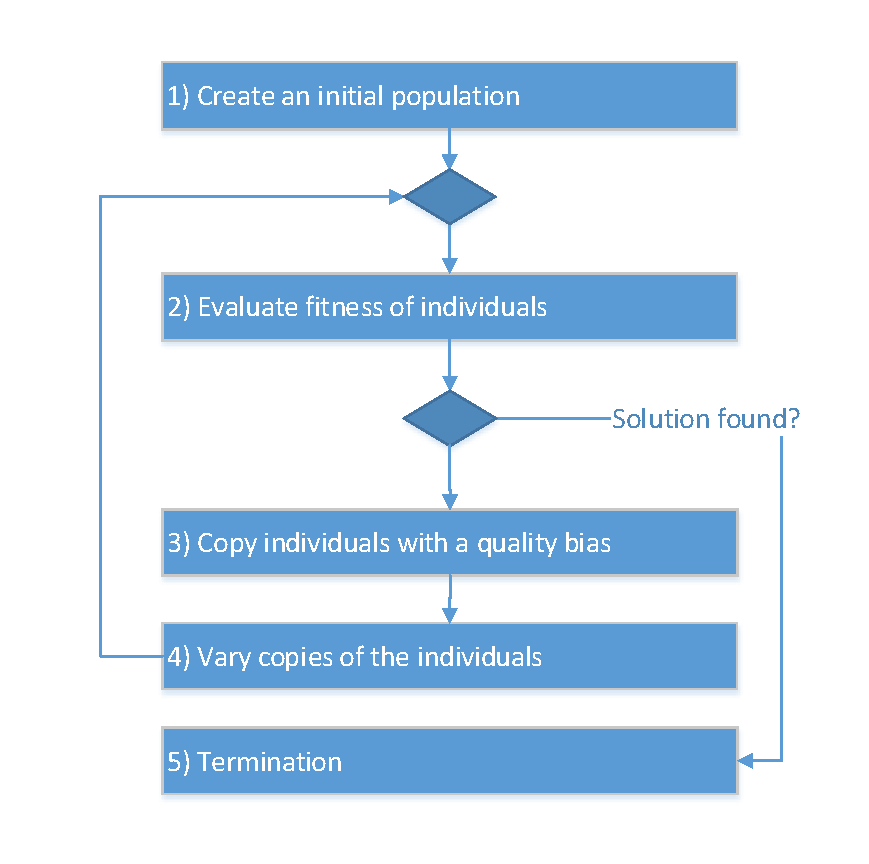
\includegraphics[scale=0.6, trim=0cm 1cm 0cm 1cm, clip=true]{Images/AlgorithmEA_GeneralOverview.pdf} 
	\caption{Evolutionary algorithm - general overview (\cite{Ashlock2004})}
	\label{figEvolutionaryAlgorithmGeneralOverview}
\end{figure}

Figure \ref{figEvolutionaryAlgorithmGeneralOverview} shows the basic control flow of an \gls{EvolutionaryAlgorithm} derived from \cite{Ashlock2004}. The first step is to create an initial \gls{Population} with a defined size representing the first \gls{Generation}. The \glspl{Individual} can be either the result of a random generation or the result from another algorithm.
The evolutionary loop then starts with the evaluation of the \glspl{Individual} using the \gls{FitnessFunction}. In the case a solution is found, the loop ends. Afterwards solution candidates are picked using a \gls{SelectionStrategy}, then are copied thereby eliminating others chosen by a \gls{ReplacementStrategy} in order to maintain a fixed \gls{Population} size. Both strategies are based on the fitness.
The final step of the loop variates the \gls{Population} by applying \glspl{GeneticOperator} on the copied \glspl{Individual}.

After describing the general behavior, a rough overview of the crucial aspects is provided in the following paragraphs.

First, the basic \glspl{SelectionStrategy} are introduced. Within \gls{RouletteWheelSelection} the probability for an \gls{Individual} to be chosen, is the proportion of its fitness to the sum of all fitness values. \Gls{TournamentSelection} creates subsets of the whole \gls{Population} and choses the best one. The size of the subset defines the selection pressure, i.e. a large subset reduces the chance for \glspl{Individual} with bad fitness to be chosen. A high selection pressure reduces the \gls{GeneticDiversity} as \glspl{CandidateSolution} with bad fitness are less likely to be exploited further.

\Glspl{ReplacementStrategy}, or also called child insertion methods, maybe of different kinds as well. A common strategy is \gls{Elitism}, where a certain number of best \glspl{Individual} is kept. Thereby, it ensures that the overall fitness never decreases but increases the chance of getting trapped in a \gls{LocalOptimum}. Those strategies may also be directly related to the \glspl{SelectionStrategy}, i.e. within the subset of a \gls{TournamentSelection} the \gls{Individual} having the worst fitness is replaced by an offspring of the one with the best fitness.

Two schemata exist for \glspl{GeneticOperator}. The first one is an unary \gls{Mutation} operator that creates a variation of an existing \gls{CandidateSolution}. It changes each \gls{Gene} of a selected \gls{Individual} with a certain probability. Basically, the idea is to perform a \gls{LocalSearch} which requires \gls{StrongCausality}. A mutation is a small change in the \gls{Genotype} and should only result in a small change in the \gls{Phenotype}. The second operator is the binary \gls{Crossover} which is applied to pairs of selected \glspl{Individual} and re-combines them to a new one. Hence, the new \gls{Individual} is located between its parents in the \gls{SearchSpace} which might be a large step. Therefore, this is a \gls{DistantSearch}.

\Glspl{EvolutionaryAlgorithm} can be quite different depending on the concrete approach. The most important and relevant ones for this thesis are presented to provide an overview for the algorithm design.

\textbf{\Gls{EvolutionaryStrategy}} \cite{rechenberg73} uses only \gls{Mutation} as an \gls{GeneticOperator}. The \glspl{Genotype} is typically based on floating-point arrays. When mutating the array, usually a normally distributed random value is added. An application of this concept might be possible in a combinatorial approach. It is probably difficult because creating a transformation based on floating point numbers has to overcome a large semantical gap.

In the case a \gls{ModelToModelTransformation} can be divided into several independent parts and each part is assigned a weight, this might be applicable.

\textbf{\Gls{GeneticAlgorithm}} \cite{holland75} is using \gls{Mutation} and \gls{Crossover} based on discrete \glspl{Genotype} (e.g. binary strings). Thus, a \gls{Mutation} is usually a bit-flip and a recombination is a one-point or two-point \gls{Crossover}.
The basic one-point \gls{Crossover} splits the parent \glspl{Genotype} into two parts at the same ``point". The new \gls{Genotype} then uses the left hand side of the first parent and the right hand side of the second parent. An extension is the two-point \gls{Crossover} which splits the parents into three parts at two ``points". Therefore, the new \gls{Genotype} is based on three parts where two are from the same parent.

This algorithm might also be applicable in a combinatorial approach.

\textbf{\Gls{GeneticProgramming}} \cite{koza92} is based on tree-representation of programs as the \gls{Genotype} which is usually the \gls{AbstractSyntaxTree}. The \gls{Mutation} and \gls{Crossover} \glspl{GeneticOperator} are therefore changing the \gls{AbstractSyntaxTree}.

Since the \gls{ModelToModelTransformation} is a program, this algorithm is presumably applicable. The major challenge is probably the \gls{LocalSearch}, as a small change in the \gls{AbstractSyntaxTree} might create a major semantic change in the program resulting in a major change in the \gls{FitnessFunction}.

\subsection{Application to Model Transformation By Example}\label{secApplicationToMTBE}

The previous subsections indicated for each algorithm a rough idea how an application to \gls{ModelTransformationByExample} could be achieved. Overall most of the presented algorithms are targeted at combinatorial problems. In order to apply those, the incomplete described problem of \gls{ModelToModelTransformation} has to be mapped to a complete problem with precise dimensions. Thereby, this reduction introduces limitations which will render the algorithm most likely in-adaptable for scenarios that are not part of this thesis. On the contrary, a \gls{GeneticProgramming} is the only one that is targeted at creating tree-based representations of programs. Hence, instances of a \gls{TransformationLanguage} can be created by such an algorithm without a reduction. However, the complexity of the presented \gls{TransformationLanguage} is an issue, that does not create difficult requirements for the \gls{Encoding} within a \gls{GeneticProgramming}, but for the \glspl{GeneticOperator} and the \gls{FitnessFunction}.

\chapter{Solution Approach}\label{chapAlgorithmicApproach}

After presenting the foundations of \gls{ModelTransformationByExample}, \glspl{ModelToModelTransformation} and meta-heuristic optimization algorithms, this chapter explains the solution approach. At first, the requirements are refined in section \ref{secRequirements}. Afterwards, the decision for the meta-heuristic optimization algorithm type is explained in section \ref{secAlgorithmTypeSelection}. Finally, an overview of the solution is presented in section \ref{secSolutionOverview} followed by a description of the used design and development process in section \ref{secDesignAndDevelopmentProcess}.

\section{Requirements}
\label{secRequirements}

The refined requirements are presented in this section based on the results of the previous chapter. At first a summary of the most important findings is listed:

\begin{itemize}
	\item The chosen definition of \gls{ModelTransformationByExample} provides little information as a guidance for the algorithm (see subsection \ref{secRelatedWorkConclusions}).
	\item A generic and precise definition of \gls{ModelToModelTransformation} is not provided by any \gls{TransformationLanguage} (see subsection \ref{secExistingModelTransformationLanguagesAndTools}). Such a definition can also not be derived from the \gls{MetaMetaModel} language \gls{MetaObjectFacility} within this thesis (see subsection \ref{secTransformationComplexity}).
\end{itemize}

The first finding results in a large and intangible \gls{SearchSpace}. Whereas, the second finding renders a complete solution of the chosen \gls{ModelTransformationByExample} problem impossible within this thesis. The refined requirements are shown in figure \ref{figRequirements} and listed in the following:

\begin{figure}[ht!]
	\centering
	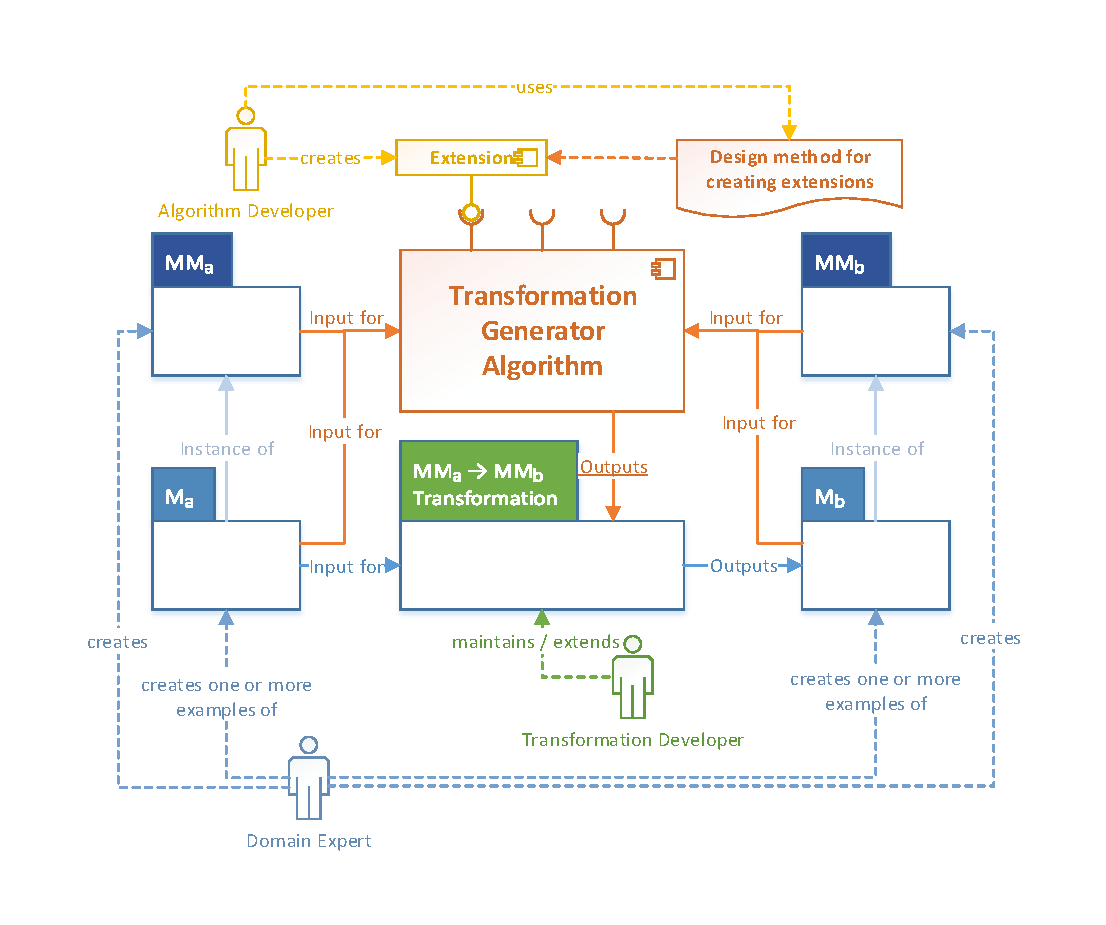
\includegraphics[scale=0.8, trim=0.5cm 1cm 0.5cm 1cm, clip=true]{Images/Requirements.pdf}
	\caption{Requirements - An extensible algorithm must be defined including a design method for creating extensions}
	\label{figRequirements}
\end{figure}

\begin{itemize}
	\item The algorithm creates a ``MM$_a$ $\rightarrow$ MM$_b$ Transformation" based on given \glspl{MetaModel} MM$_a$ and MM$_b$ provided by a domain expert. 
	\item It is guided by manually created M$_a$ - M$_b$ example-pairs, also created by a domain expert. No further information is provided like details about the mapping from M$_a$ to M$_b$.
	\item Since a complete algorithm cannot be created due to the incomplete definition of \glspl{ModelToModelTransformation}, the algorithm cannot guarantee a solution. Hence, the algorithm must be extensible by providing generic extension parameters.
	\item The algorithm must consider large \glspl{SearchSpace}.
	\item A design method for creating extensions must be defined. It guides the algorithm developer. In particular, the method must consider the problem of non-termination in large \glspl{SearchSpace}.
	\item The created ``MM$_a$ $\rightarrow$ MM$_b$ Transformation" might not be a complete solution, since the algorithm is incomplete. Thus, the transformation must be maintainable by a transformation developer.
	\item A solution for the transformation scenarios defined in chapter \ref{chapM2MScenarios} must be found within a few hours, which is considered an acceptable time.
\end{itemize}

\section{Meta-Heuristic Optimization Algorithm Type Selection}
\label{secAlgorithmTypeSelection}

Before presenting the solution overview, this section at first explains the decision for an algorithm type. This decision has an impact on all other aspects of the algorithm design. As a result of the previous insights there are two possible directions which are presented in the following.

The first one (Direction A) is to use the definition of a \gls{TransformationLanguage} to create instances of itself. The second one (Direction B) is to divide the general problem of \glspl{ModelToModelTransformation} into smaller units, which are then being solved by meta-heuristic optimization algorithms.

While direction A is the more direct one, because it could more or less immediately be tackled by a \gls{GeneticProgramming} (see subsection \ref{secEvolutionaryAlgorithms}), it has also the greater chance of facing the problem of non-termination very soon. This is due to the fact that \glspl{TransformationLanguage} are complex, which has been outlined in subsection \ref{secExistingModelTransformationLanguagesAndTools}. Combined with the results of section \ref{secAlgorithms} the definition of a \gls{FitnessFunction}, which converges to a solution might become difficult. Most of the created instances are probably far away from any kind of solution ending up in a random search.

This issue could be avoided in the fist place by direction B. The idea is to split the problem of \glspl{ModelToModelTransformation} into different, algorithmic-friendly sub-problems or units. For example one unit might be matching \glspl{Class} from M$_a$ to M$_b$ and another one matching the \glspl{Property}. The former may be a combinatorial problem while the latter is a generative one. So an assignment of the ideal algorithm for each unit is possible.

Nevertheless, also direction B has two major downsides. On the one hand, the overall aggregation of the units is an ``ordinary" algorithm that has to be created from scratch. This algorithm is not based on a meta-heuristic and hence, lacks a theoretical foundation. On the other hand, creating units is a huge challenge on its own. In particular, there is a risk that the algorithm-friendly language has fundamental limitations, which renders it useless in common scenarios that have not been considered in the design phase. Consequently, an extension might require changing the existing algorithm. Thus, the extensibility of the algorithm with an acceptable effort cannot be guaranteed. Furthermore, following this approach leads to a focus on the definition of a \gls{TransformationLanguage} and the aggregation of the units and not on the actual algorithms.

After looking at the advantages and disadvantages of both directions the risk of designing an own algorithm-friendly, unit-based \gls{TransformationLanguage} has been considered as too high, because it might very likely exceed the scope of this thesis and move the focus in a different direction. Hence, the decision is to take direction A using a \gls{GeneticProgramming}. 

% with the restriction, to avoid the non-termination issue as far as possible. Only \glspl{Class}, \glspl{Association} and \glspl{Property} without any calculations are transformed. The calculation of the latter introduces, as already mentioned in section \ref{secRelatedWork}, at lot of additional complexity. In order to link \glspl{Class} of MM$_a$ to MM$_b$ it is assumed that there is a \gls{Property} ``Name" that is equal in \glspl{Object} of M$_a$ and M$_b$ for semantically identically \glspl{Class} (see section \ref{secRelatedWork}).

%If the algorithm works, then \glspl{Property} are taken into account. Otherwise, it is the task of the developer to extend the transformation. An additional requirement in direction A is therefore that the result must be readable and maintainable manually because it might be incomplete. This is considered when designing and evaluating the algorithm.

\section{Solution Overview}
\label{secSolutionOverview}

This section provides an overview of the solution. At first the general concept is explained and afterwards an overview of the central entities of the solution. As explained within the requirements, the algorithm will be incomplete, but must be extensible as well as the created \glspl{ModelToModelTransformation}. Furthermore, the large \gls{SearchSpace} must be considered since it might prevent the algorithm from terminating with a solution at all or in an acceptable time.

\begin{figure}[ht!]
	\centering
	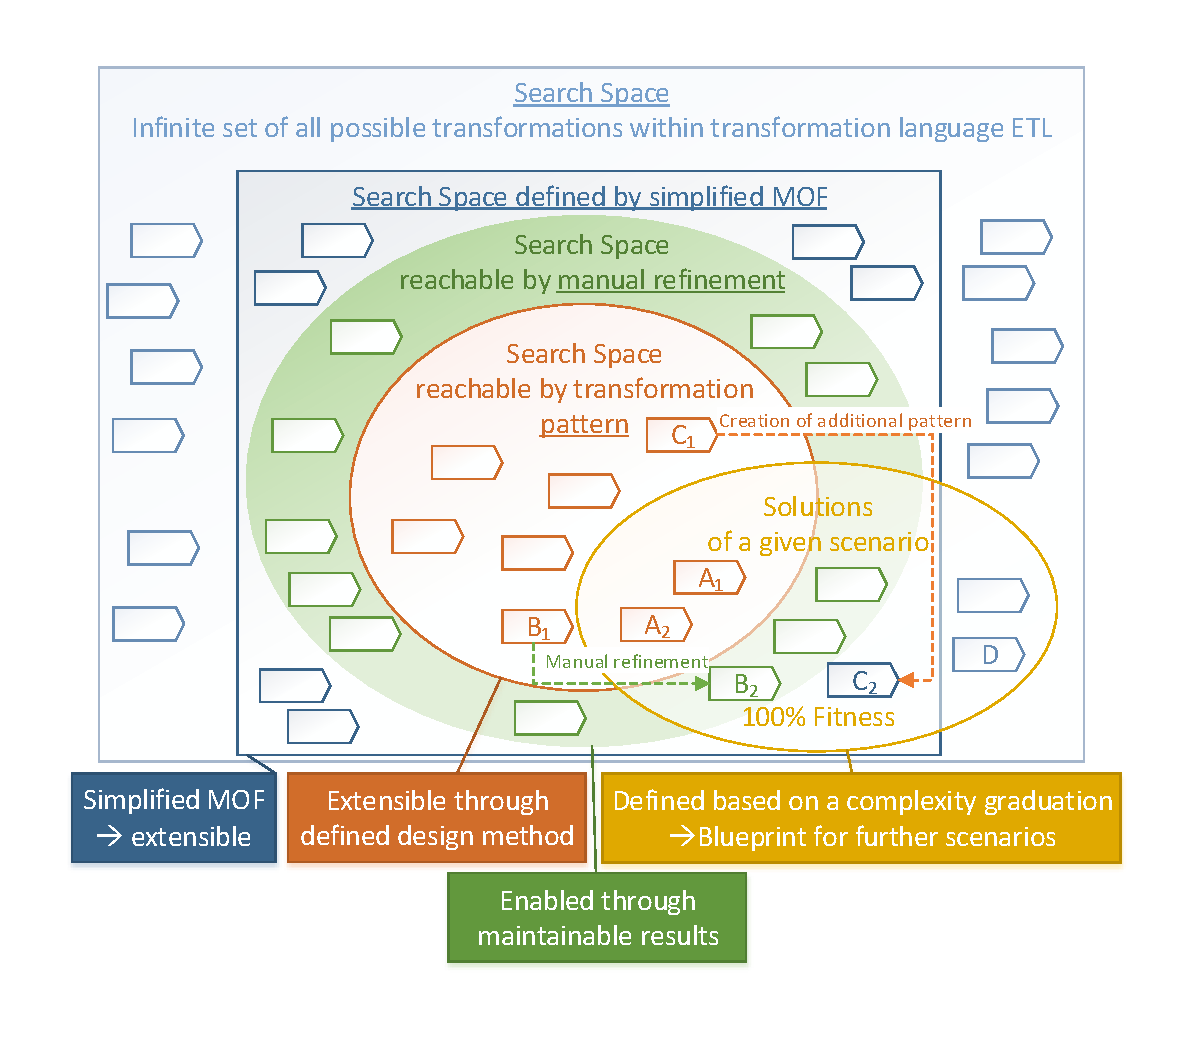
\includegraphics[scale=0.7, trim=0cm 1cm 0cm 1cm, clip=true]{Images/SearchSpaceDivideAndConquer.pdf} 
	\caption{Search Space - Overview of the divide-and-conquer approach}
	\label{figSearchSpaceDivideAndConquer}
\end{figure}

Figure \ref{figSearchSpaceDivideAndConquer} provides an overview of the general concept to fulfill those requirements. The presented key ideas are listed in the following: %It shows transformations as small blocks. Solutions for a given transformation scenario can be

\begin{itemize}
\item The whole \gls{SearchSpace} is defined by the infinite set of all possible transformations within the \gls{EpsilonTransformationLanguage}.
\item In order to limit the possible transformations considered in this thesis, the \gls{MetaMetaModel} language \gls{MetaObjectFacility} is simplified (see subsection \ref{secModelLanguage}). Thereby, the possible \glspl{MetaModel} are limited which can be solved by a limited number of transformations. The simplified \gls{MetaObjectFacility} is the foundation for the systematic construction of the representative transformation scenarios. Within figure \ref{figSearchSpaceDivideAndConquer}, the solution D of the given transformation scenario is therefore out-of-scope. Nevertheless, the simplified \gls{MetaObjectFacility} can be extended towards \gls{MetaObjectFacility}.
\item The \gls{GeneticProgramming} is based on transformation patterns, which are the foundation of its \glspl{GeneticOperator}. Those patterns are a small subset of the \gls{EpsilonTransformationLanguage}. Therefore, they cannot create all solutions for a given scenario. In figure \ref{figSearchSpaceDivideAndConquer} only the solutions A$_1$ and A$_2$ can be created by the algorithm. 
\item Transformation patterns are well-defined transformation concepts and avoid creating incomprehensible solutions. Thereby, a transformation developer can for example modify the transformation B$_1$ into B$_2$. The former was close to the solution, while the latter is a 100\% solution of the given scenario. In general, a manual modification could result in any transformation i.e. also C$_2$. This requires more knowledge and effort compared to small modifications which are therefore only expected.
\item Transformation patterns can be extended using the defined design method. For example, the algorithm might terminate with the transformation C$_1$ which is not a solution of the given scenario. By adding an additional pattern, the algorithm becomes capable of modifying this transformation to C$_2$, which is a solution. 
\item Furthermore, most of the transformations in the \gls{SearchSpace} are likely to produce low-quality output. It can not be distinguished with the given inputs for the algorithm. Hence, the algorithm has no guidance and the termination with a solution - even when theoretically reachable - is unlikely. The patterns also limit this problem, when designed according to the specified design method.
\end{itemize}

\begin{figure}[ht!]
	\centering
	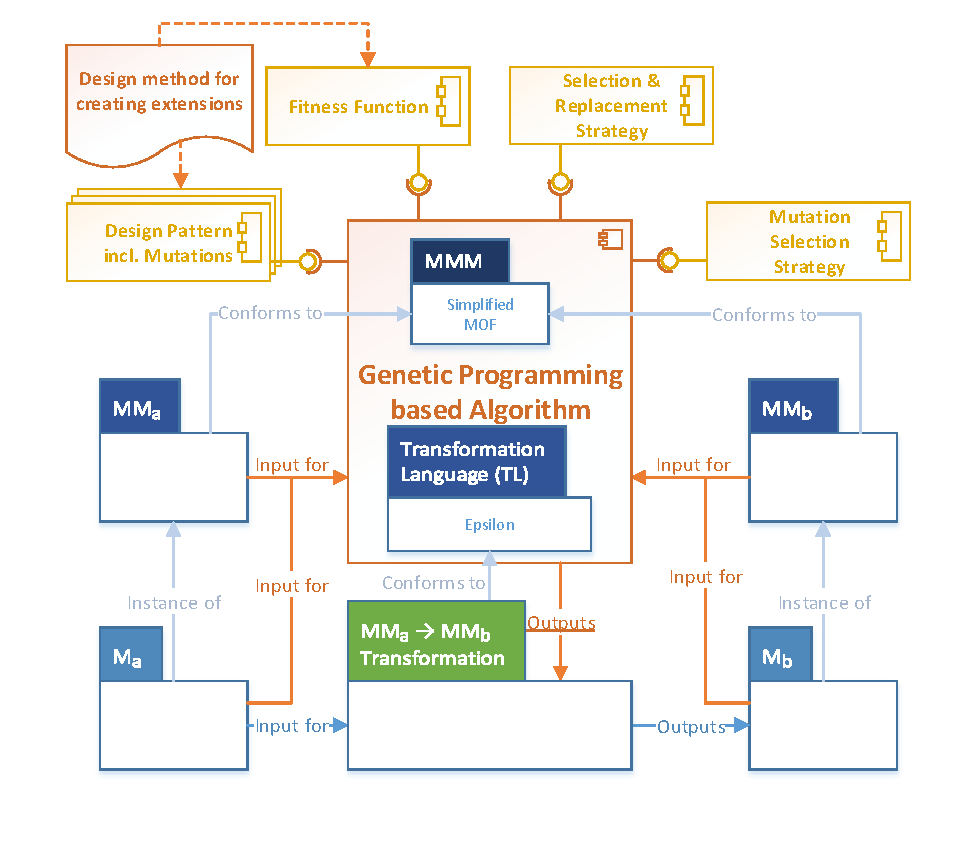
\includegraphics[scale=0.8, trim=0.5cm 1.2cm 0.5cm 0cm, clip=true]{Images/Solution.pdf}
	\caption{Overview of the central entities of the solution}
	\label{figSolution}
\end{figure}

After explaining the general concept, the central entities of the solution are presented in figure \ref{figSolution}. The algorithm is based on a \gls{GeneticProgramming} as decided in the previous section \ref{secAlgorithmTypeSelection}. The input and output \glspl{MetaModel} are instances of the simplified \gls{MetaMetaModel} \gls{MetaObjectFacility} (see subsection \ref{secModelLanguage}). Created ``MM$_a$ $\rightarrow$ MM$_b$ Transformation" conform to the selected \gls{TransformationLanguage} \gls{EpsilonTransformationLanguage} (see subsection \ref{secExistingModelTransformationLanguagesAndTools}). Besides the previously mentioned transformation patterns also other aspects of the algorithm are exchangeable and/or extensible components. Transformation patterns are the foundation for the \glspl{Mutation} required by the \gls{GeneticProgramming}. Since there are many patterns resulting in many \glspl{Mutation}, a mutation selection strategy is required. The \gls{FitnessFunction} is necessary to rate transformations created by the algorithm. As explained in subsection \ref{secEvolutionaryAlgorithms}, the algorithm is based on a \gls{SelectionStrategy} and \gls{ReplacementStrategy}, which is also an exchangeable component.

The design method describes the creation of additional transformation patterns and the required extensions of the \gls{FitnessFunction}. Since additional patterns extend the reachable transformations, those transformations also create other types of output \glspl{Model}. Hence, the \gls{FitnessFunction} which rates the transformation depending on the output, must be adopted to reflect the new types as well.

\section{Design and Development Process}
\label{secDesignAndDevelopmentProcess}

Since this thesis tries to solve a software engineering problem with a meta-heuristic optimization algorithm using a new approach, there is no reference design process available, yet. Therefore, this section provides an overview of the followed design and development process shown in figure \ref{figDevelopmentProcess}. The x-axies of the matrix contains the software development process phases Design, Implementation, Unit Test and Integration Test / Evaluation. On the y-axis are the entities of the algorithm. The size of each step from one to nine in figure \ref{figDevelopmentProcess} indicates the spent effort. The following list provides an overview of the design and development process of the algorithm entities:

\begin{figure}[htb]
	\centering
	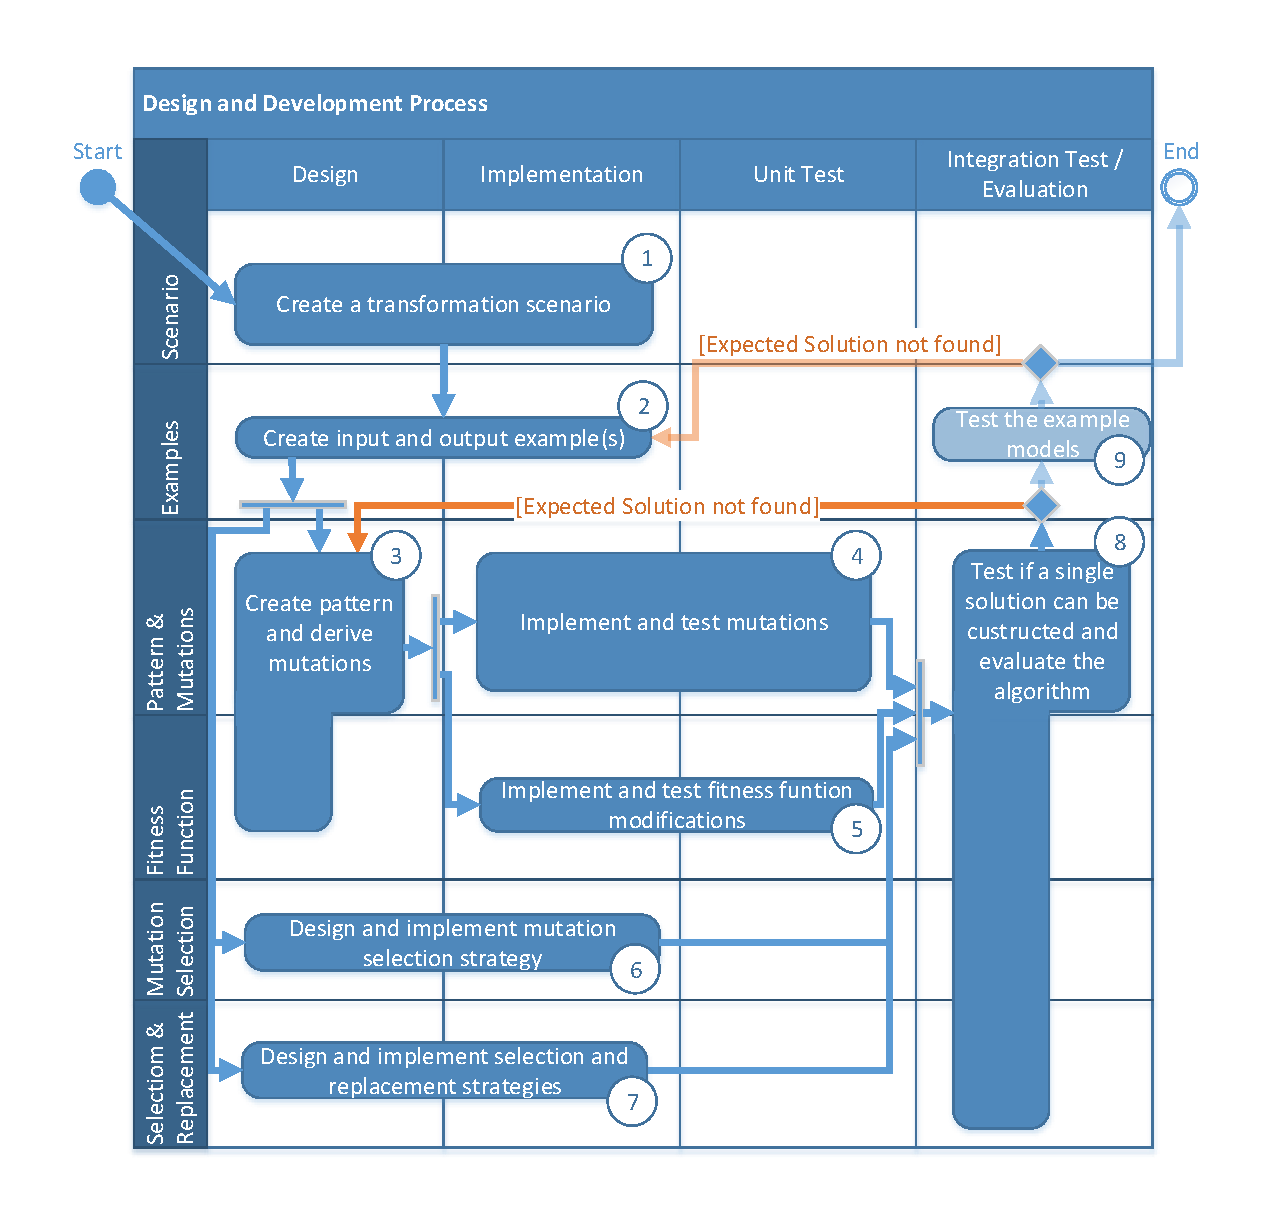
\includegraphics[scale=0.7, trim=0cm 1cm 0cm 1cm, clip=true]{Images/DevelopmentProcess.pdf} 
	\caption{Design and development process - overview of the created entities and phases. The size of the activities indicates the effort.}
	\label{figDevelopmentProcess}
\end{figure}

\begin{enumerate}
	\item Create a transformation scenario. It includes the transformation problem defined by two \glspl{MetaModel}. Furthermore, a reference transformation from the first to the second \gls{MetaModel} is specified as a guideline for the pattern design. In order to control the complexity of the scenario, the complexity analysis presented in subsection \ref{secTransformationComplexity} is used. The created scenarios are explained in chapter \ref{chapM2MScenarios}.
	\item For each scenario, at least one input and expected output \gls{Model} has to be created. Those are also presented in chapter \ref{chapM2MScenarios}.
	\item Afterwards, the reference transformation is analyzed and missing transformation patterns are added or existing patterns are extended. Based on the patterns, the \glspl{Mutation} are derived which are used by the algorithm. Also the \gls{FitnessFunction} is extended to reflect the new kinds of output created by the added \glspl{Mutation}. The design method required to create these entities is presented in section \ref{secMutationAndFitnessFunctionDesignProcess}, the implemented patterns are described in \ref{secPatternAndMutations} and the \gls{FitnessFunction} in section \ref{secFitnessFunctions}.
	\item Following the software development process, the \glspl{Mutation} are implemented and tested individually (see section \ref{secRealizationOfMutations} and section \ref{secMutationProcess}).
	\item The same applies to the \gls{FitnessFunction}, which is also tested using selected transformations derived from the reference transformation (see section \ref{secMutationProcess}).
	\item The Mutation Selection Strategies have a design and implementation phase, but are not tested individually. They are relatively simple and the effect is only observable in the integration test of all components (see section \ref{secMutationSelectionStrategies}).
	\item The same applies to the Selection and Replacement Strategies (see section \ref{secSelectionReplacementStrategies}).
	\item Finally all components are assembled. The integration test for each scenario is to verify that at least one solution can be constructed. Afterwards, the general performance and the quality of the created transformations is evaluated. The results are explained in chapter \ref{chapEvaluation}.
	\item Within the evaluation also flaws in the examples are detected (see subsection \ref{secMaintainabilityOfResults}). Hence, improvements of the examples are required. It avoids the possibility of considering example-specific results as a solution. Since example improvements do not affect the algorithm design, it is not in scope of this thesis.
\end{enumerate}
\glsresetall
\chapter{Representative Model-to-Model-Transformation Scenarios}\label{chapM2MScenarios}

In order to create an automatic \gls{TransformationGenerator}, it is necessary to define representative test scenarios. Each scenario consists of two \glspl{MetaModel} and at least two semantically identical example \glspl{Model} of those (see chapter \ref{chapFoundations}). 

Designing software systems usually involves the analysis of structure and behavior, hence those categories have been chosen for the scenarios (see chapter \ref{chapIntroduction}), to show the relevance of the transformations. However, in terms of the transformation complexity the category does not matter.

The starting point is a simple structural scenario, while the complex one is a behavioral scenario.

\section{Simple Structural Scenario}\label{secM2MScenarioStructuralSimple}

As a result of the analysis in section \ref{secTransformationComplexity}, the simple structural example requires only a 1:1 transformation of \glspl{MetaObjectFacility} \glspl{Class}, \glspl{Association} and ``Name"-\glspl{Property}.

\begin{figure}[htb]
	\centering
	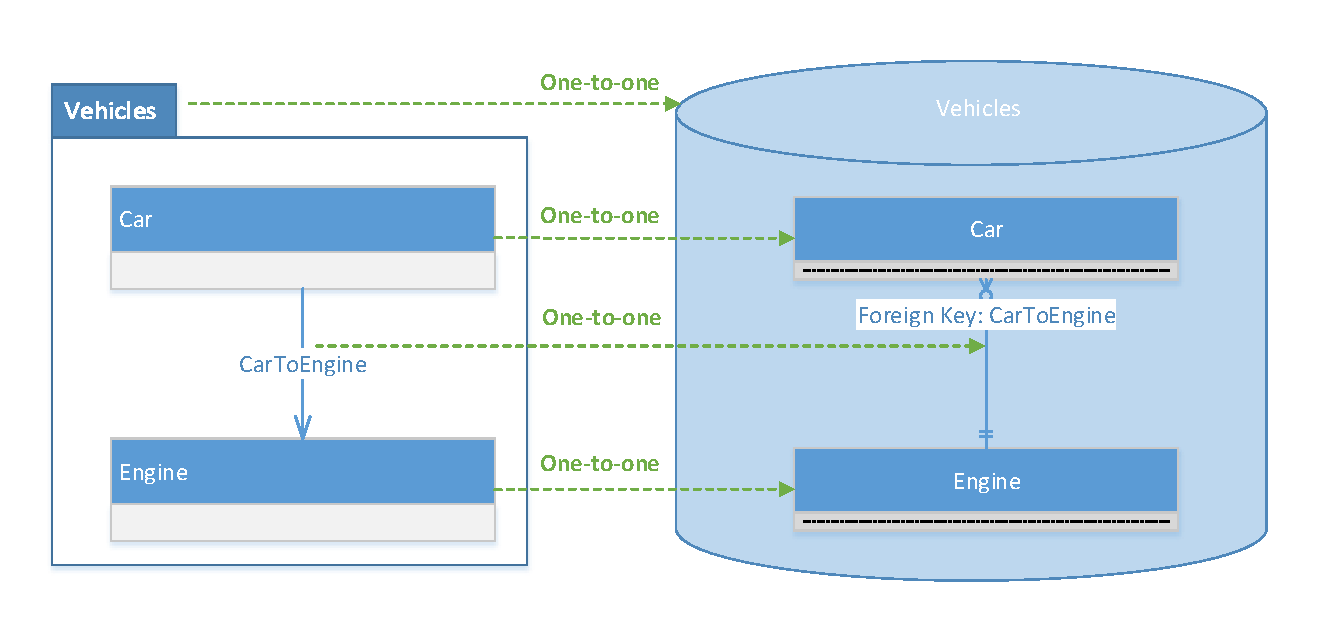
\includegraphics[scale=0.6, trim=0cm 1cm 0cm 1cm, clip=true]{Images/ScenarioStructuralSimpleOverview.pdf} 
	\caption{Simple transformation scenario overview with a \Gls{UnifiedModelingLanguage} \gls{ClassDiagram} \gls{Model} on the left side and an equivalent \gls{RelationalSchema} \gls{Model} on the right side, both in \gls{ConcreteSyntax}}
	\label{figScenarioStructuralSimpleOverview}
\end{figure}

A common scenario in the field of \gls{ModelDrivenDevelopment} is the already mentioned transformation of a \gls{UnifiedModelingLanguage} \gls{ClassDiagram} to a \gls{RelationalSchema}. Figure \ref{figScenarioStructuralSimpleOverview} shows the transformation scenario based on an example. In order to have 1:1 transformations on the \gls{MetaModel} and \gls{Model} level, only the core concepts are used. The \gls{ClassDiagram} consists of a package ``Vehicles", the \glspl{Class} ``Car" and ``Engine", as well as an \gls{Association} between those. The \gls{RelationalSchema} has a database schema ``Vehicles", the tables ``Car" and ``Engine", and a foreign-key in table ``Car" which points to the table ``Engine".

In the following paragraphs the \glspl{MetaModel}, the \gls{ModelToModelTransformation} and the example \glspl{Model} are presented.

It has to be pointed out that the terms \gls{Class} and \gls{Property} exist in both, the \glspl{MetaObjectFacility} and the \gls{ClassDiagram}.

The reduced \gls{UnifiedModelingLanguage} \gls{ClassDiagram} \gls{MetaModel} shown in figure \ref{figScenarioStructuralSimpleUmlClassMetaModel} consists of a ``UmlPackage" that contains ``UmlClasses" and ``UmlAssociations". The former may be associated by the latter to another ``UmlClass". Therefore, a ``UmlAssociation" has a ``Source" and ``Target" association.

\begin{figure}[htb]
	\centering
	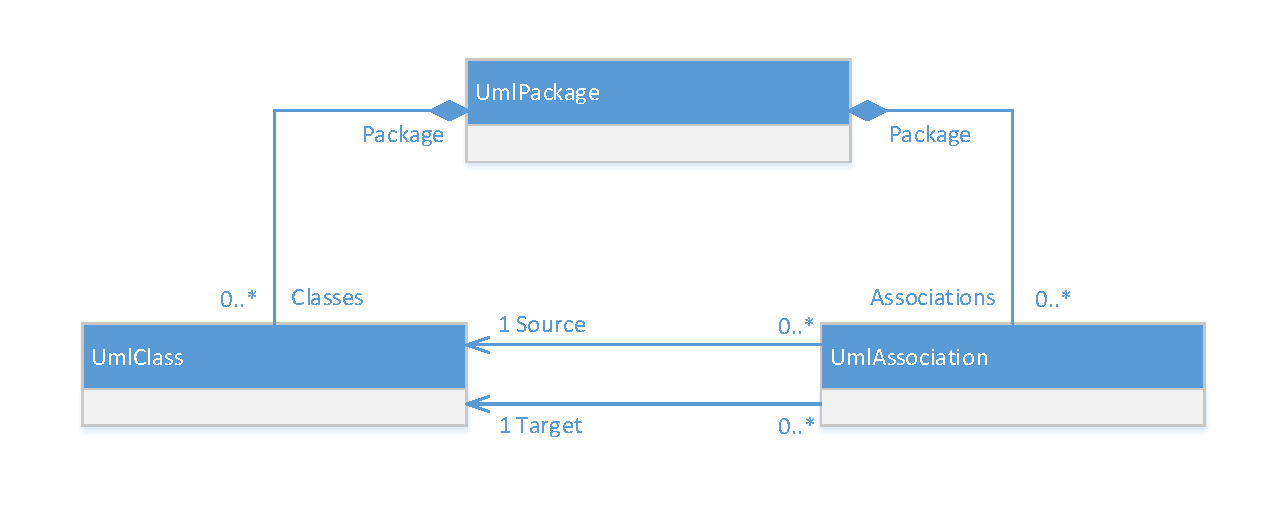
\includegraphics[scale=0.6, trim=0cm 1cm 0cm 1cm, clip=true]{Images/ScenarioStructuralSimpleUmlClassMetaModel.pdf} 
	\caption{\Gls{UnifiedModelingLanguage} \gls{ClassDiagram} - simplified \gls{MetaModel}}
	\label{figScenarioStructuralSimpleUmlClassMetaModel}
\end{figure}

The simplified \gls{RelationalSchema} \gls{MetaModel} is shown in figure \ref{figScenarioStructuralSimpleRelationalMetaModel}. It includes a ``RelationalSchema" that contains ``RelationalTables". The latter may refer to others of the same kind via a ``RelationalForeignKey" that has an association named ``ReferencedTable". The difference to the \gls{UnifiedModelingLanguage} \gls{ClassDiagram} \gls{MetaModel} is that the ``ForeignKey" is only associated to the owning ``Table" and not to the ``RelationalSchema". Hence, this association has no equivalence and requires no mapping.

\begin{figure}[htb]
	\centering
	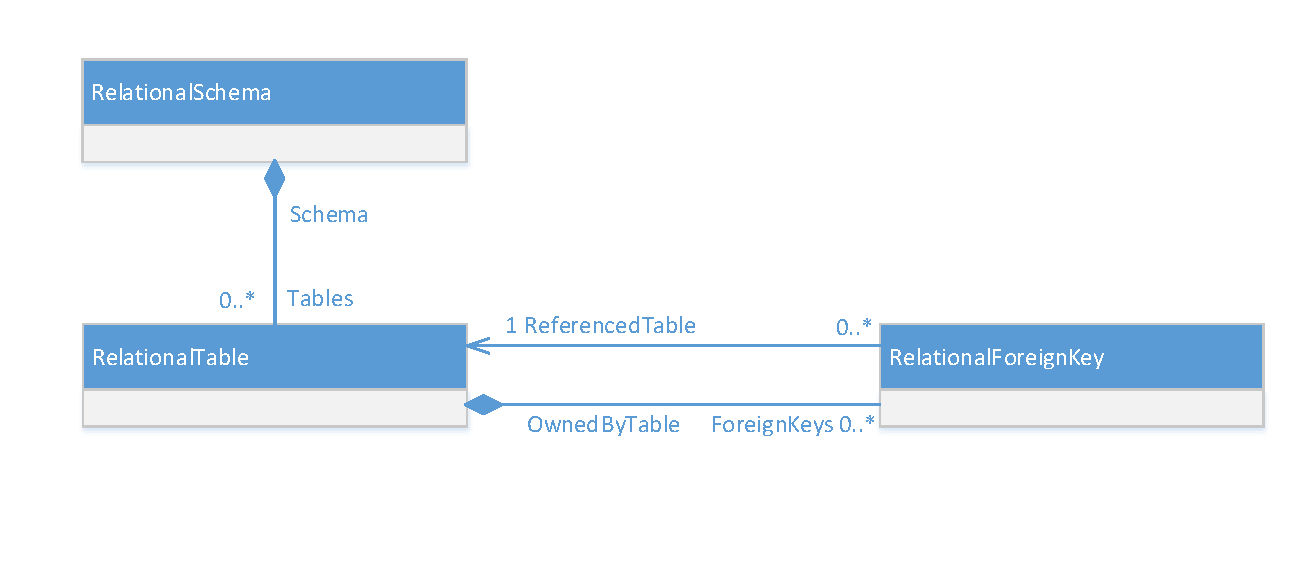
\includegraphics[scale=0.6, trim=0cm 1cm 0cm 1cm, clip=true]{Images/ScenarioStructuralSimpleRelationalMetaModel.pdf} 
	\caption{\Gls{RelationalSchema} - simplified \gls{MetaModel}}
	\label{figScenarioStructuralSimpleRelationalMetaModel}
\end{figure}

A transformation that converts the first \gls{MetaModel} into the second one is presented in listing \ref{lstETLSimpleExample}. This is a valid transformation, but it is not the only one, since there are other possible solutions. The presented one contains three rules, one for each \gls{MetaObjectFacility} \gls{Class}, resulting in the \glspl{TransformationRule} ``UmlPackage To RelationalSchema", ``UmlClass To RelationalTable", ``UmlAssociation To RelationalForeignKey". All rules have a mapping for the ``Name" \gls{Property}. Additionally, ``UmlClass To RelationalTable" maps the associated ``UmlPackage" of the ``UmlClass" to the corresponding ``RelationalSchema" of the created ``RelationalTable" with the keyword ``equivalent". The rule ``UmlAssociation To RelationalForeignKey" contains mappings for the ``Source" and ``Target" to the corresponding \glspl{Property} of the \gls{RelationalSchema}.

\begin{lstlisting}[language=ETL,caption={Simple \gls{UnifiedModelingLanguage} \gls{ClassDiagram} to simple \gls{RelationalSchema} \gls{ModelToModelTransformation} in \gls{ConcreteSyntax} of \gls{EpsilonTransformationLanguage}},label={lstETLSimpleExample}]
rule UmlPackageToRelationalSchema
  	transform umlPackage : Source!UmlPackage
  	to relationalSchema : Target!RelationalSchema {
  
  	relationalSchema.Name = umlPackage.Name; 
}

rule UmlClassToRelationalTable 
	transform umlClass : Source!UmlClass
	to relationalTable : Target!RelationalTable {
	
	relationalTable.Name = umlClass.Name;
	relationalTable.Schema = umlClass.Package.equivalent();
}

rule UmlAssociationToRelationalForeignKey
	transform umlAssociation : Source!UmlAssociation
	to relationalForeignKey : Target!RelationalForeignKey {
	
	relationalForeignKey.Name = umlAssociation.Name;
	relationalForeignKey.OwnedByTable = umlAssociation.Source.equivalent();
	relationalForeignKey.ReferencedTable = umlAssociation.Target.equivalent();	
}
\end{lstlisting}

In order to identify a transformation with the \gls{TransformationGenerator} also at least one example \gls{Model} pair for those two \glspl{MetaModel} has to be defined. It is required for them to be semantically equivalent. Figure \ref{figScenarioStructuralSimpleUmlClassModel1} shows a \gls{Model} conforming to the \Gls{UnifiedModelingLanguage} \gls{ClassDiagram} \gls{MetaModel}. It contains a ``UmlPackage" named ``Vehicles" that defines the context. Inside this package are a ``Car" and an ``Engine" which are ``UmlClasses". Those are associated by a ``Car 2 Engine" ``UmlAssociation". 

\begin{figure}[htb]
	\centering
	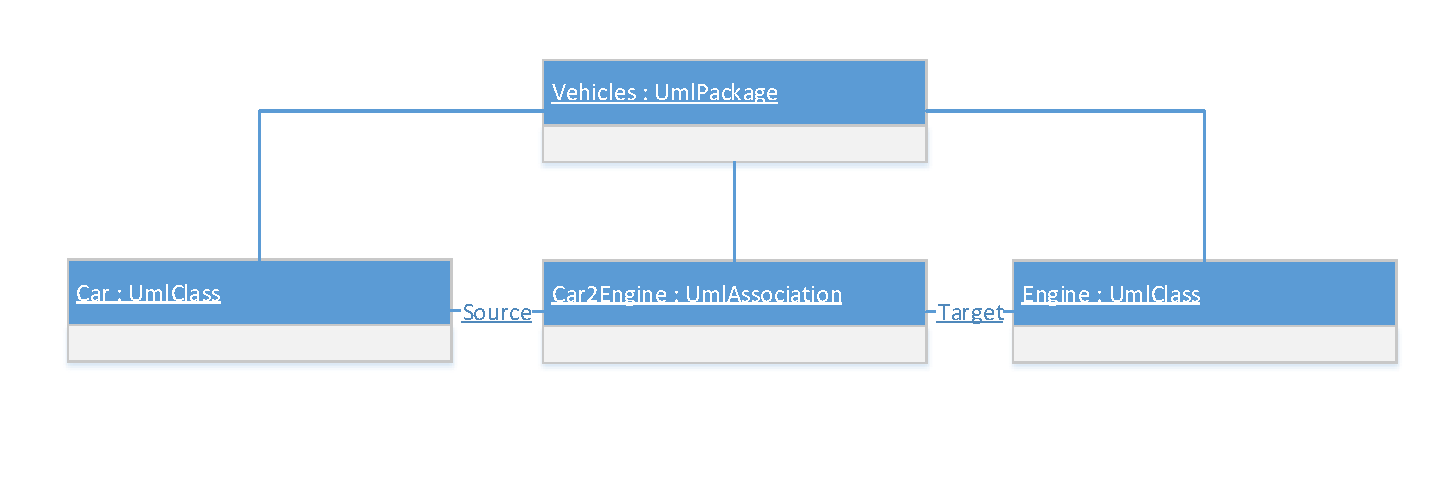
\includegraphics[scale=0.6, trim=0cm 1cm 0cm 1cm, clip=true]{Images/ScenarioStructuralSimpleUmlClassModel1.pdf} 
	\caption{\Gls{UnifiedModelingLanguage} \gls{ClassDiagram} example \gls{Model}}
	\label{figScenarioStructuralSimpleUmlClassModel1}
\end{figure}

The semantically identical \gls{Model}, conforming to the \gls{RelationalSchema} \gls{MetaModel}, is presented in figure \ref{figScenarioStructuralSimpleRelationalModel1}.

%It has to be pointed out that the containment relationship between the ``RelationalTable" ``Car" and the ``Car 2 Engine" ``RelationalForeignkey" is only visible in the presentation of the \gls{MetaModel}.

\begin{figure}[htb]
	\centering
	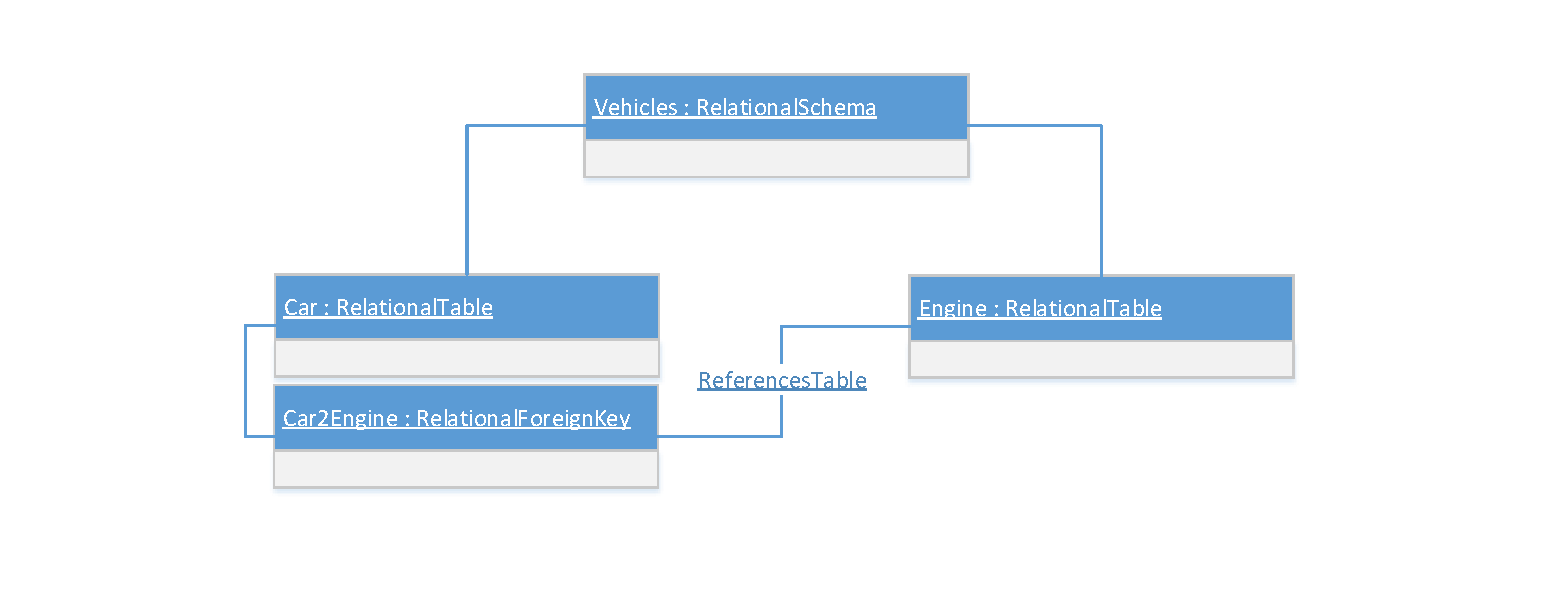
\includegraphics[scale=0.6, trim=0cm 1cm 0cm 1cm, clip=true]{Images/ScenarioStructuralSimpleRelationalModel1.pdf} 
	\caption{\Gls{RelationalSchema} example \gls{Model}}
	\label{figScenarioStructuralSimpleRelationalModel1}
\end{figure}

\section{Complex Behavioral Scenario}\label{secM2MScenarioBehavioralComplex}

According to the identified complexity levels in section \ref{secTransformationComplexity}, the complex example contains 1:N relations, relations that exist only under certain conditions and attribute calculations on M1.

The scenario is also common in the field of \gls{SoftwareEngineering}, which is necessary in order to show the relevance of the transformation. Compiler design is based on the concept of finite-\glspl{StateMachine}, which basically defines states and transitions between those. Since this is a low-level concept, the instances can become very large and hence difficult to read for humans. The concept of hierarchical-\glspl{StateMachine} has been introduced, which adds composite states that contain states. Thereby, the number of explicit transitions is reduced. Nevertheless, hierarchical-\glspl{StateMachine}, called complex-\glspl{StateMachine} in the following, cannot always be executed and therefore must be transformed back into (flat)-\glspl{StateMachine}, called simple-\glspl{StateMachine} in the following.

\begin{figure}[htb]
	\centering
	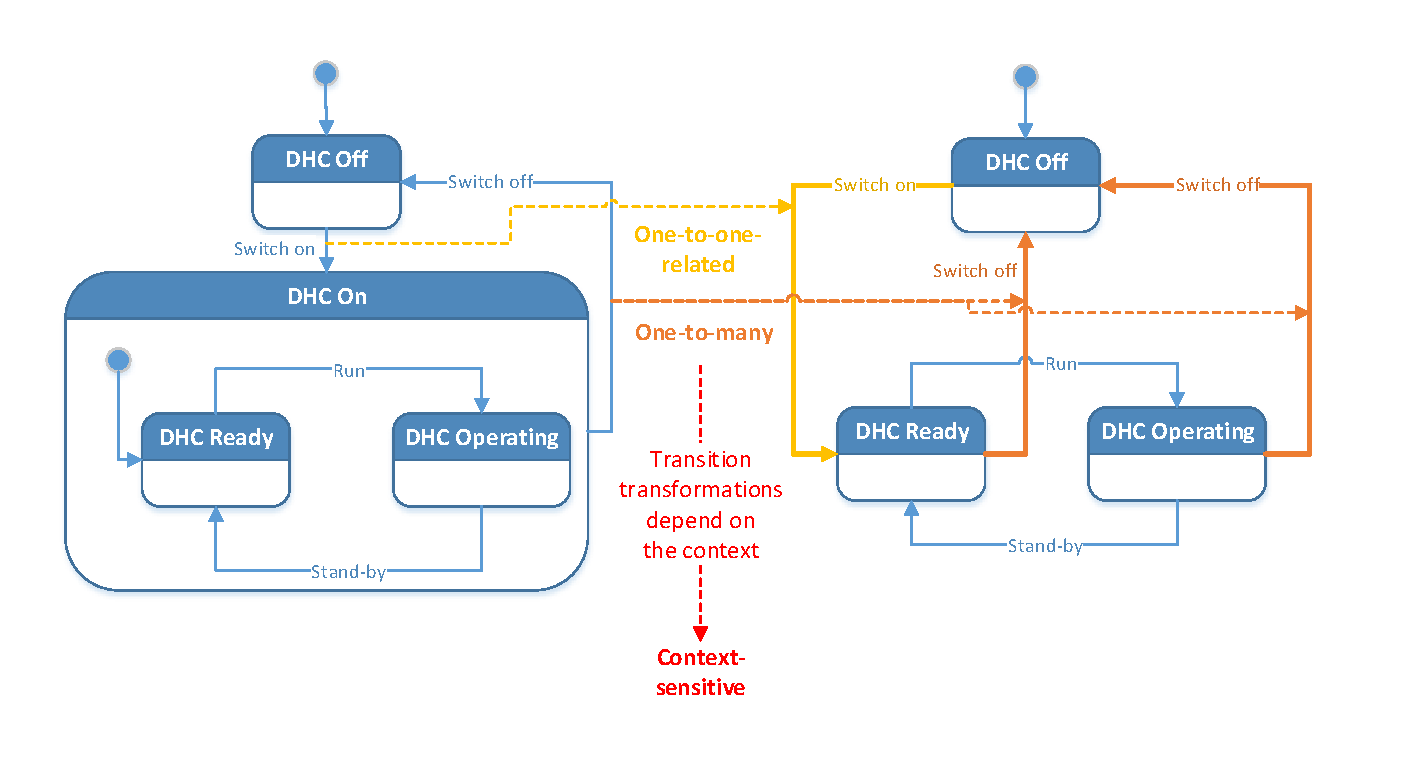
\includegraphics[scale=0.6, trim=0cm 1cm 0cm 1cm, clip=true]{Images/ScenarioBehavioralStateMachineTransformationOverview.pdf} 
	\caption{Complex transformation scenario overview with \glspl{StateMachine} in \gls{ConcreteSyntax}}
	\label{figScenarioBehavioralStateMachineTransformationOverview}
\end{figure}

Figure \ref{figScenarioBehavioralStateMachineTransformationOverview} shows an example of such a transformation and highlights the additional transformation challenges. The ``DHC" example is derived from \cite{Gerth2014} which is based on \cite{Engels2004} and models a warehouse management system. In the reduced example the ``DHC" only has the state ``DHC Off" and the complex state ``DHC On". Within the latter the machine starts in the state ``DHC Ready" and can switch to ``DHC Operating" and back. Since the complex state contains a transition to ``DHC Off", the machine can be turned off in every state inside.

The simple \gls{StateMachine} on the right hand side does not have the complex state. Therefore, the transition from ``DHC Off" to ``DHC On" points instead directly to ``DHC Ready". This results in a 1:1 transformation on M2 and M1, but the target of the transition is not the equivalent \gls{Class}, which does not exist anymore. Rather, the target is the initial state within in the composite state, therefore this is called ``One-to-one related". The outgoing transition from ``DHC On" to ``DHC Off" has to be replaced by a transition from every state inside the composite state which is called ``One-to-many". Since there are different kinds of transformations required for transitions, depending on the context of those, a third new challenge is called ``Context-sensitive" transformations.

\begin{figure}[htb]
	\centering
	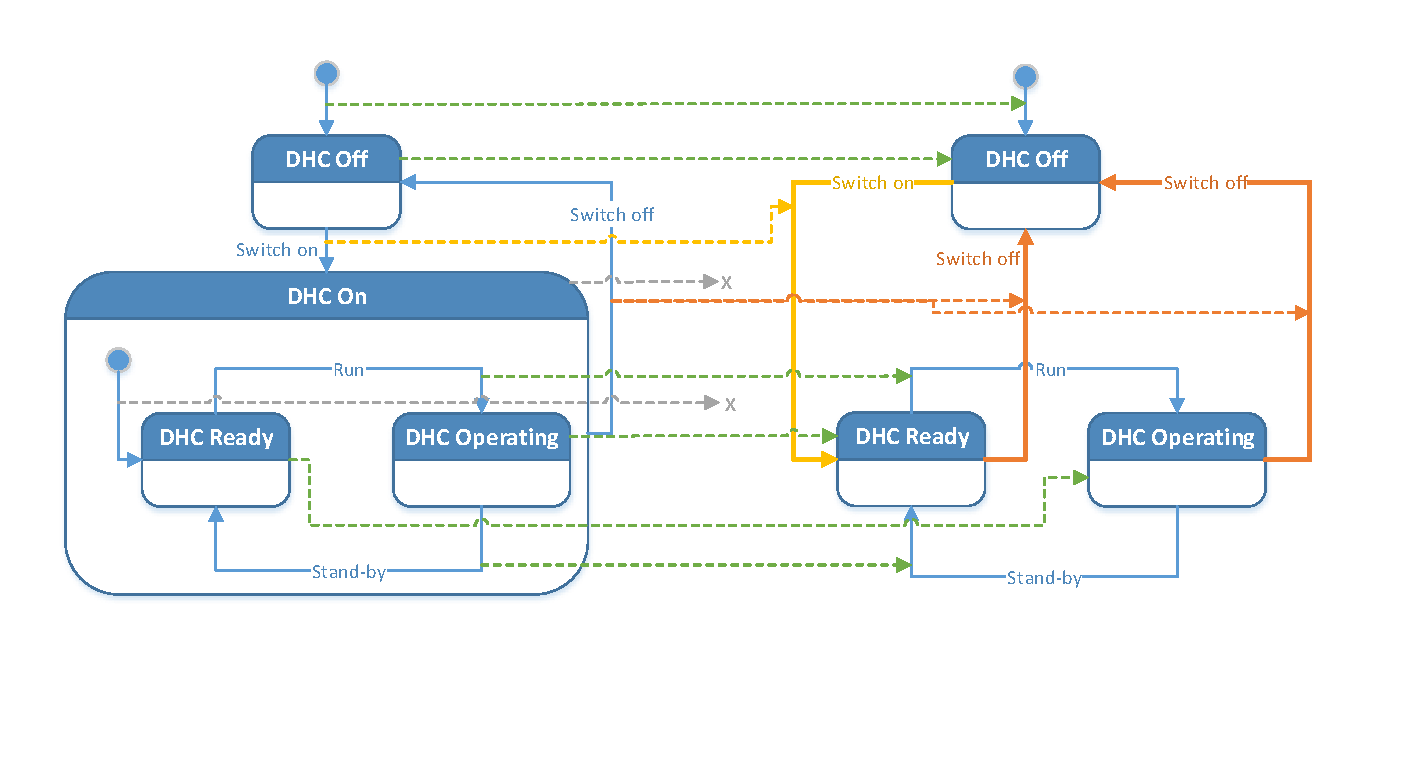
\includegraphics[scale=0.6, trim=0cm 1cm 0cm 1cm, clip=true]{Images/ScenarioBehavioralStateMachineTransformationOverview2.pdf} 
	\caption{Complex transformation scenario overview with \glspl{StateMachine} in \gls{ConcreteSyntax}}
	\label{figScenarioBehavioralStateMachineTransformationOverview2}
\end{figure}

While figure \ref{figScenarioBehavioralStateMachineTransformationOverview} highlights only the new transformation types, figure \ref{figScenarioBehavioralStateMachineTransformationOverview2} provides an overview of all required transformations for this example. Since the composite state has no equivalence, this results in a ``to zero" transformation. All other parts are transformed 1:1 on the \gls{MetaObjectFacility} \gls{Object} level, i.e. the state ``DHC Off". 
% transitions are not 1:1, the related \glspl{Association} change in these cases, too. An example is ``DHC Off", where in the complex-\gls{StateMachine} is one incoming and one outgoing transition, while in the simple-\gls{StateMachine} there are two incoming.

Following the same structure as in the simple scenario, in the next paragraphs the \glspl{MetaModel}, \glspl{ModelToModelTransformation} and the example \glspl{Model} are presented.

\begin{figure}[htb]
	\centering
	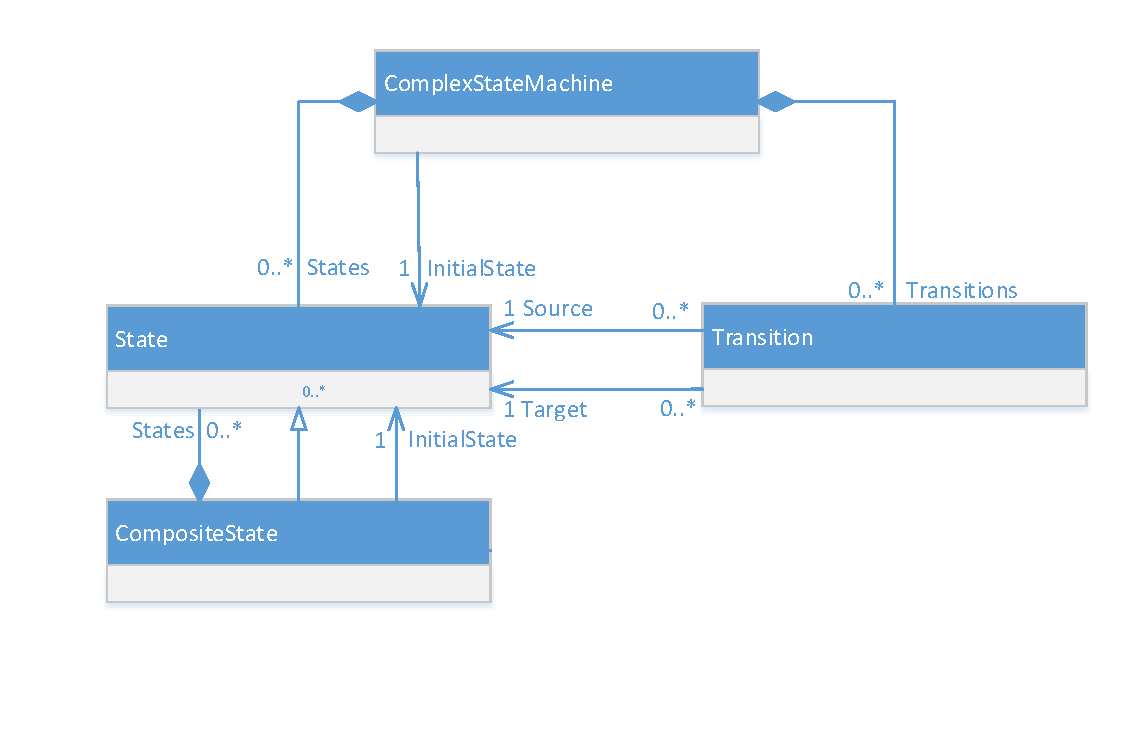
\includegraphics[scale=0.6, trim=0cm 1cm 0cm 1cm, clip=true]{Images/ScenarioBehavioralComplexStateMachine.pdf} 
	\caption{Complex State Machine - simplified \Gls{UnifiedModelingLanguage} \gls{StateMachine} \gls{MetaModel} with Composite States}
	\label{figScenarioBehavioralComplexStateMachine}
\end{figure}

The \gls{MetaModel} of the complex-\gls{StateMachine} is depicted in figure \ref{figScenarioBehavioralComplexStateMachine}. A ``ComplexStateMachine" consists of ``States" and ``Transitions" and defines an ``InitialState". A ``State" is connected by directed ``Transitions" to others and can also be a ``ComplexState". In this case it also contains ``States" and defines an ``InitialState".

\begin{figure}[htb]
	\centering
	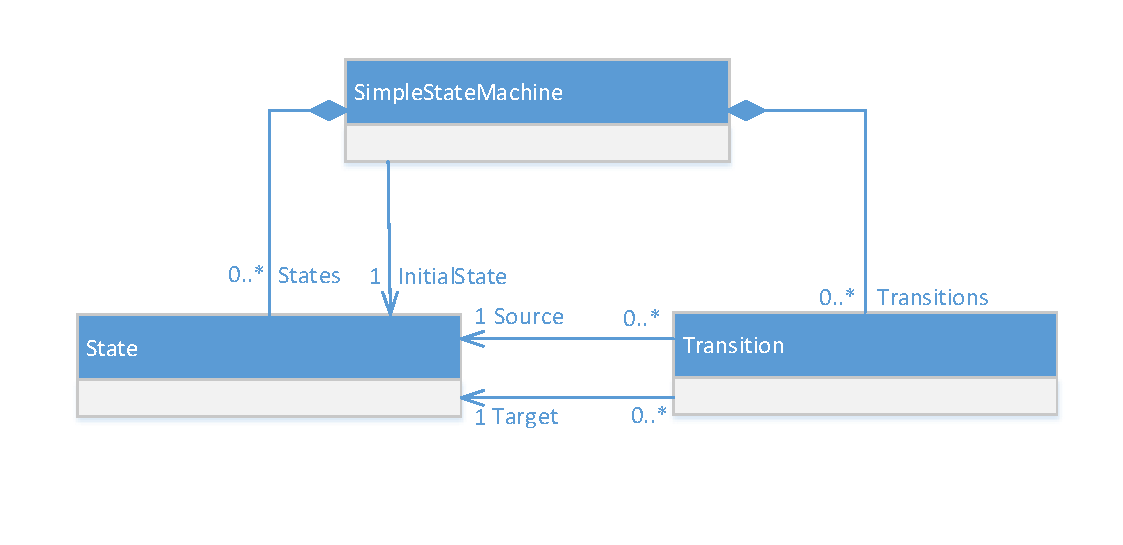
\includegraphics[scale=0.6, trim=0cm 1cm 0cm 1cm, clip=true]{Images/ScenarioBehavioralComplexSimpleStateMachine.pdf} 
	\caption{Simple State Machine - simplified \Gls{UnifiedModelingLanguage} \gls{StateMachine} \gls{MetaModel} without Composite States}
	\label{figScenarioBehavioralComplexSimpleStateMachine}
\end{figure}

The \gls{MetaModel} of the simple-\gls{StateMachine} is shown in figure \ref{figScenarioBehavioralComplexSimpleStateMachine}. It is identical to the complex type, except that the ``ComposisteState" is missing and that the name is ``SimpleStateMachine".

A \gls{ModelToModelTransformation} for those two \glspl{MetaModel} is defined in listing \ref{lstETLComplexExample}. There are multiple different transformations possible, depending on the approach. In this case, rules are defined for all \glspl{Class}, resulting in ``ComplexStateMachine To SimpleStateMachine", ``State To State", ``Transition To Transition". 

Since a transition is transformed differently depending on the context, there exists one rule for each, resulting in the additional rules ``TransitionPointingToComplexState To Transition" and ``TransitionFromComplexState To ManyTransitions". Another approach could be to handle all situations within one rule. Hence the used \gls{EpsilonTransformationLanguage} contains a concept called ``guards", which allows the definition of pre-conditions per rule, separate rules are defined to improve the readability. This solves the ``Context-dependent" challenge.

The ``One-to-one related" issue is solved in the rule ``TransitionPointingToComplexState To Transition", which covers all incoming ``Transitions" of a ``ComplexState". It defines a transformation from the ``InitialState" of the targeted ``ComplexState" towards the ``Target"-\gls{Property}. This change is also reflected in the mapping of the ``Name"-\gls{Property}. Another possible solution is to map the ``InitialState" of the ``ComplexState" by creating a further distinction of the ``State To State" rule. Since this does not remove the requirement for the ``TransitionPointingToComplexState To Transition" rule, this solution would result in a more complicated transformation.

The ``One-to-many" challenge is handled within the rule ``TransitionFromComplexState To ManyTransitions", which handles all outgoing ``Transitions" of a ``ComplexState". Here, the ``States" of the ``ComplexState" are enumerated and for each a new ``Transition" is created. The ``Source" is the current ``State", while the ``Target" is equivalent to the one of the handled ``Transition". This relationship is reflected in the ``Name" of the new ``Transition". As well as in the previous case, this can also be solved by a dedicated ``State To State" rule, which would result in a less comprehensible transformation.

\begin{lstlisting}[language=ETL,caption={Complex State Machine to Simple State Machine \gls{ModelToModelTransformation} in \gls{ConcreteSyntax} of \Gls{EpsilonTransformationLanguage}},label={lstETLComplexExample}]
rule ComplexStateMachineToSimpleStateMachine
	transform complexStateMachine : Source!ComplexStateMachine
	to simpleStateMachine : Target!SimpleStateMachine {
	
	simpleStateMachine.Name = complexStateMachine.Name;
	simpleStateMachine.InitialState = 
								complexStateMachine.InitialState.equivalent();
}

rule StateToState
	transform sourceState : Source!State
	to targetState : Target!State {
	
	targetState.Name = sourceState.Name;	
	targetState.SimpleStateMachine = 
								sourceState.ComplexStateMachine.equivalent();
}

rule TransitionToTransition
	transform sourceTransition : Source!Transition
	to targetTransition : Target!Transition {
	guard : 	not sourceTransition.Target.isTypeOf(Source!CompositeState)
		    and not sourceTransition.Source.isTypeOf(Source!CompositeState) 
	
	targetTransition.SimpleStateMachine = 
								sourceTransition.ComplexStateMachine.equivalent();
	targetTransition.Name = sourceTransition.Name;
	targetTransition.Source = sourceTransition.Source.equivalent();	
	targetTransition.Target = sourceTransition.Target.equivalent();
}

rule TransitionPointingToComplexStateToTransition
	transform sourceTransition : Source!Transition
	to targetTransition : Target!Transition { 
	guard : sourceTransition.Target.isTypeOf(Source!CompositeState)
			and not sourceTransition.Source.isTypeOf(Source!CompositeState)
	
	targetTransition.Name = sourceTransition.Source.Name + " -> " + 
							sourceTransition.Target.InitialState.Name;
	targetTransition.Source = sourceTransition.Source.equivalent();
	targetTransition.Target = sourceTransition.Target.InitialState.equivalent();

	targetTransition.SimpleStateMachine = 
								sourceTransition.ComplexStateMachine.equivalent();
}

rule TransitionFromComplexStateToManyTransitions
	transform sourceTransition : Source!Transition
	to targetTransitions : Sequence(Target!Transition) {
	guard : sourceTransition.Source.isTypeOf(Source!CompositeState)
			and not sourceTransition.Target.isTypeOf(Source!CompositeState)

	for(sourceState in sourceTransition.Source.States) {
		var targetTransition = new Target!Transition;
		targetTransitions.add(targetTransition);
		
		targetTransition.Name = sourceState.Name + " -> " + 
								sourceTransition.Target.Name;
		targetTransition.Source = sourceState.equivalent();
		targetTransition.Target = sourceTransition.Target.equivalent();
		
		targetTransition.SimpleStateMachine = 
								sourceTransition.ComplexStateMachine.equivalent();
	}
}
\end{lstlisting}

The described \gls{ModelToModelTransformation} results in the following changes of a \gls{Model}, which is the example used to guide the \gls{TransformationGenerator}. Those are in the \gls{AbstractSyntax}, to be able to present all involved \gls{MetaObjectFacility} elements as they are handled by the \gls{TransformationGenerator}.

\begin{figure}[htb]
	\centering
	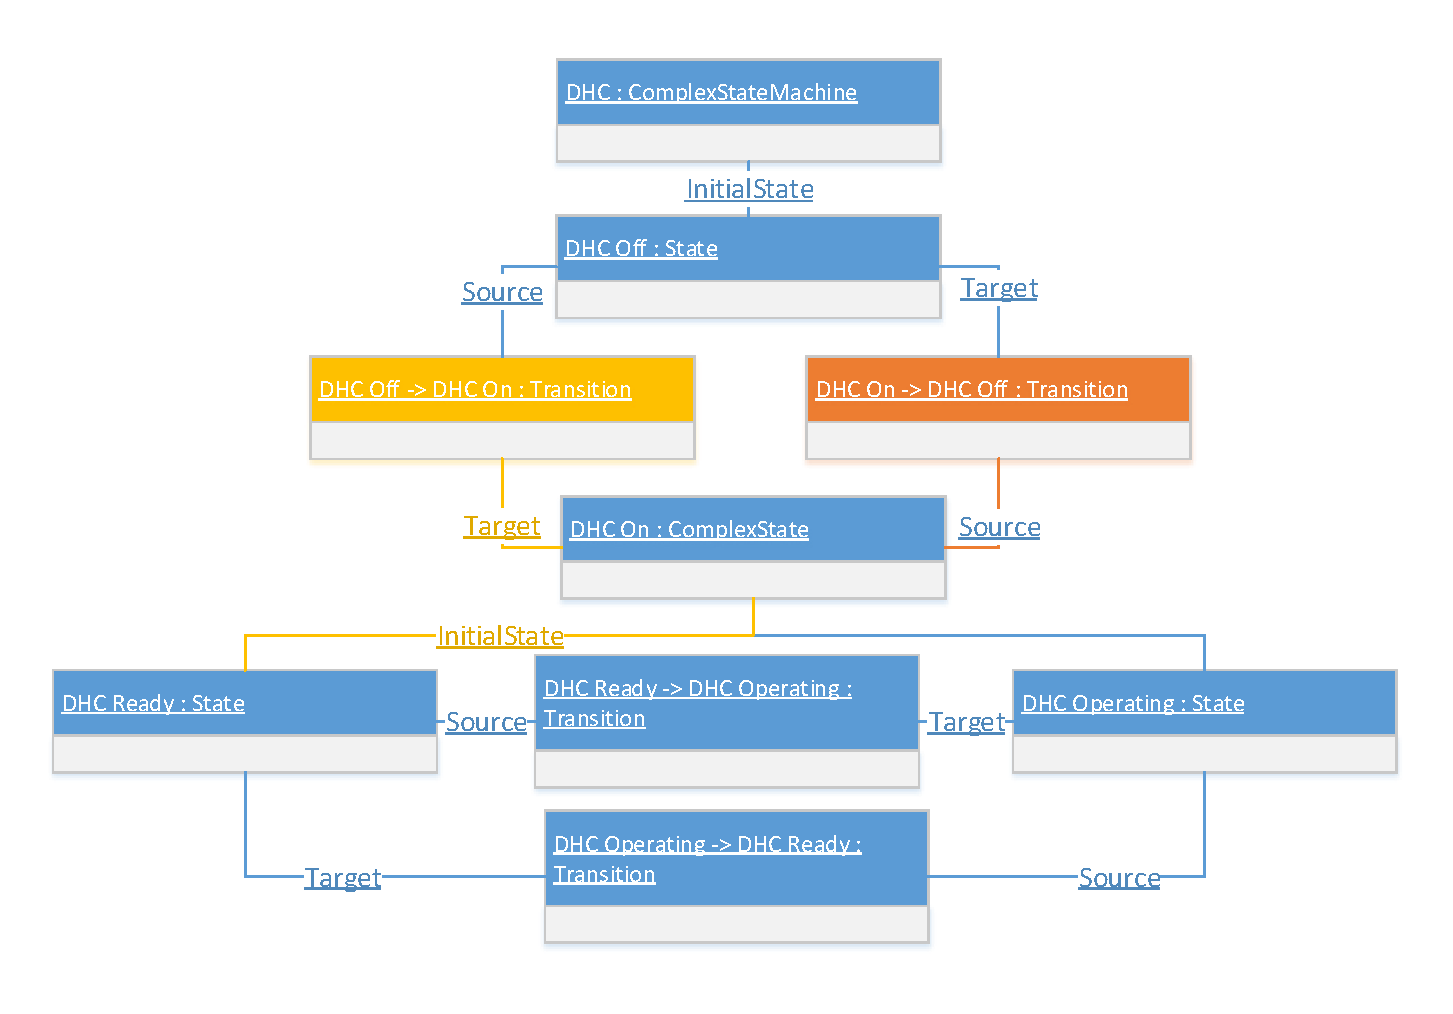
\includegraphics[scale=0.6, trim=0cm 1cm 0cm 1cm, clip=true]{Images/ScenarioBehavioralComplexStateMachineModel1.pdf} 
	\caption{Complex State Machine example \gls{Model} in \gls{AbstractSyntax} (without the associations from the ComplexStateMachine to all other \glspl{Object})}
	\label{figScenarioBehavioralComplexStateMachineModel1}
\end{figure}

Figure \ref{figScenarioBehavioralComplexStateMachineModel1} shows the input \gls{Model} M$_a$ and figure \ref{figScenarioBehavioralComplexSimpleStateMachineModel1} the output \gls{Model} M$_b$, based on the already introduced example. The highlighted parts correspond to the previously defined challenges in figure \ref{figScenarioBehavioralStateMachineTransformationOverview}.

The ``TransitionPointingToComplexState To Transition"-rule changes the ``DHC Off  $\rightarrow$  DHC On"-"Transition" into ``DHC Off  $\rightarrow$  DHC Ready". ``TransitionFromComplexState To ManyTransitions" replaces the ``DHC On  $\rightarrow$  DHC Off"-"Transition" with the two inner ``States" of the ``ComplexState".

\begin{figure}[htb]
	\centering
	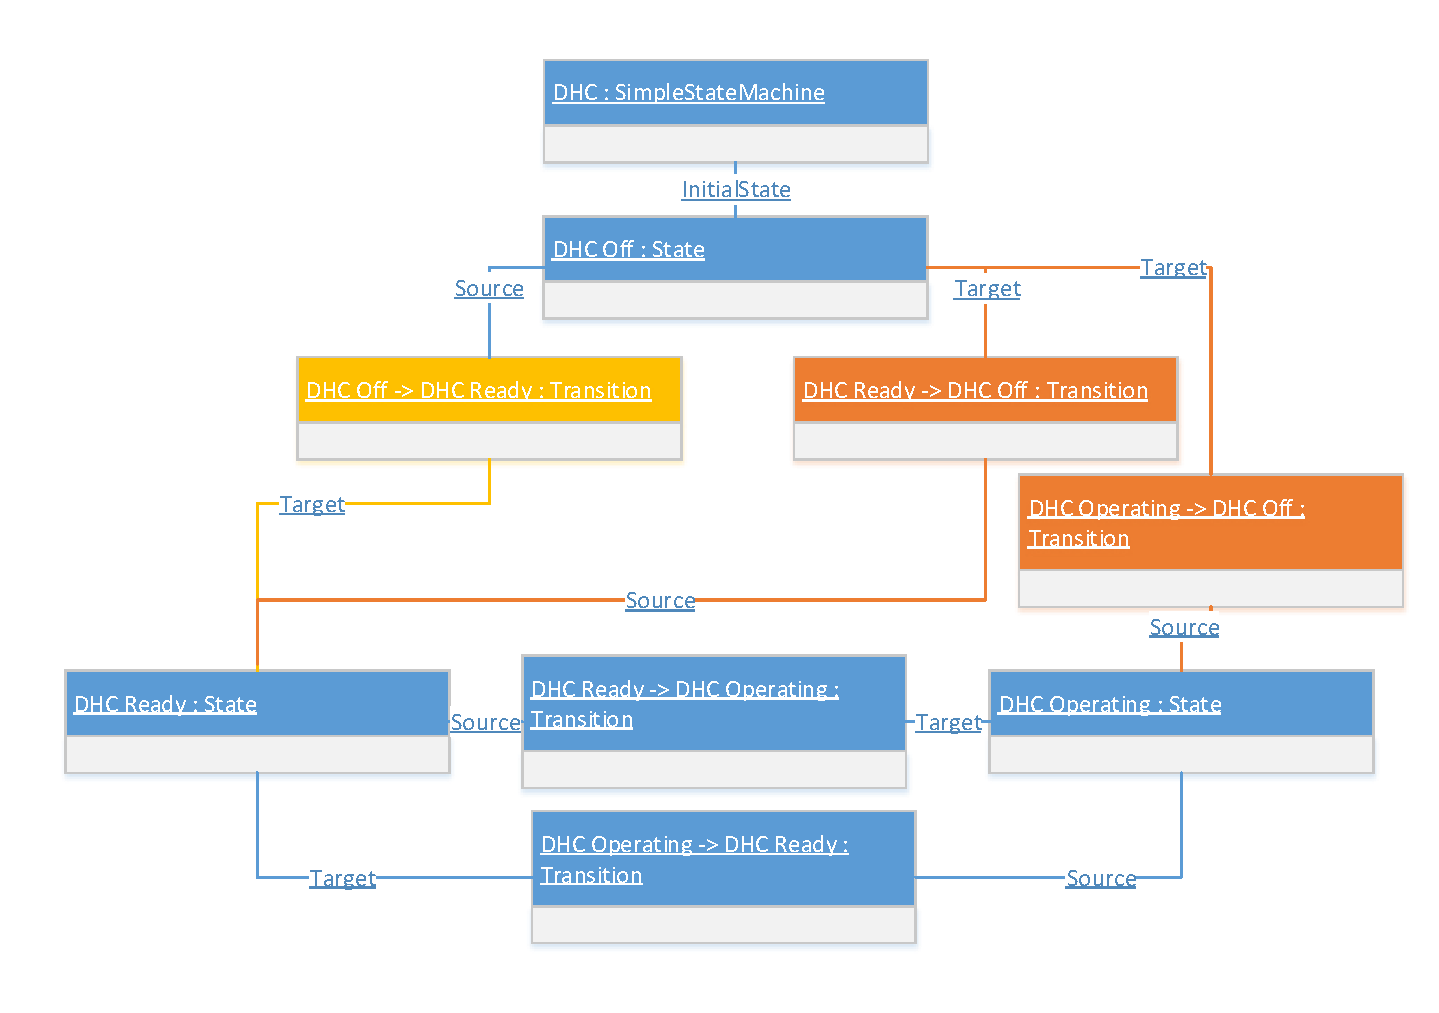
\includegraphics[scale=0.6, trim=0cm 1cm 0cm 1cm, clip=true]{Images/ScenarioBehavioralComplexSimpleStateMachineModel1.pdf} 
	\caption{Simple State Machine example \gls{Model} in \gls{AbstractSyntax} (without the associations from the SimpleStateMachine to all other \glspl{Object})}
	\label{figScenarioBehavioralComplexSimpleStateMachineModel1}
\end{figure}




\glsresetall
\chapter{Algorithm Design}\label{chapAlogrithmDesign}

The approach is based on a \gls{GeneticProgramming}, as decided in chapter \ref{chapAlgorithmicApproach}. Section \ref{secAlgorithmOverview} describes the algorithm. In section \ref{secMutationAndFitnessFunctionDesignProcess} details about the design method of the core entities are provided. Those are \glspl{Mutation} and \glspl{FitnessFunction}. Section \ref{secPatternAndMutations} explains the \glspl{Mutation} used in the algorithm with its associated pattern. The further sections describe the alternative strategies within fitness evaluation (section \ref{secFitnessFunctions}), selection and replacement (section \ref{secSelectionReplacementStrategies}) and mutation selection (section \ref{secMutationSelectionStrategies}).

\section{Algorithm Overview}
\label{secAlgorithmOverview}

The used \gls{EvolutionaryAlgorithm} has been derived from \cite{Ashlock2004} and is shown in its modified version in figure \ref{figEvolutionaryAlgorithm}. It splits up into six phases, distributed among four components, which are described after the general design decisions in the following. 

\begin{figure}[htb]
	\centering
	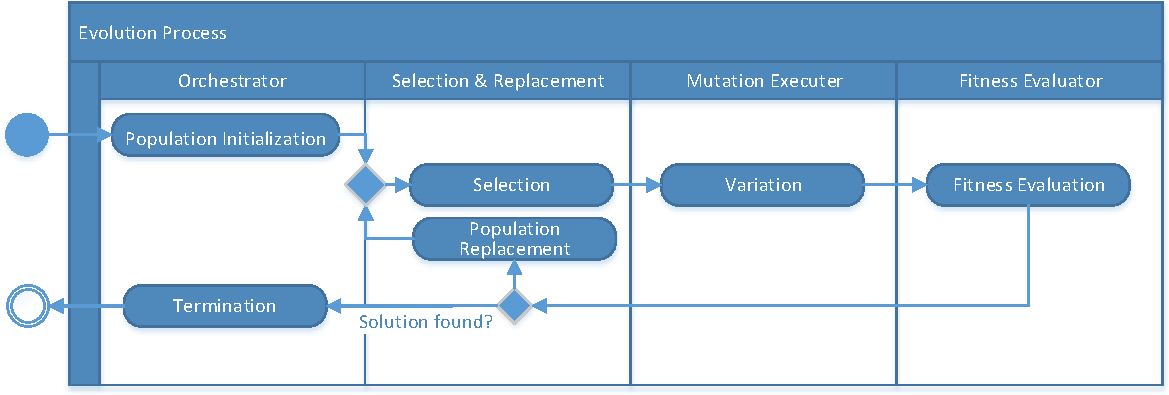
\includegraphics[scale=0.75]{Images/AlgorithmEA.pdf} 
	\caption{Evolutionary Algorithm (\cite{Ashlock2004})}
	\label{figEvolutionaryAlgorithm}
\end{figure}

As explained in section \ref{secTransformationComplexity}, the problem of generating \glspl{ModelToModelTransformation} is difficult to tackle. Since an \gls{EvolutionaryAlgorithm} itself is a general construct, it does not provide guidance for this particular issue. Therefore, the complexity is captured by a tailored method, which uses complex \glspl{GeneticOperator} that create \glspl{ModelToModelTransformation} based on design patterns.

The common approach in the field of \glspl{EvolutionaryAlgorithm} is to handle the complexity with the \gls{FitnessFunction}. Using it for this problem would result in generic \glspl{GeneticOperator} that are only based on the information provided by the \gls{TransformationLanguage} and \gls{MetaObjectFacility} definition. Hence, the created \glspl{ModelToModelTransformation} are not comprehensible and would cause only in very rare cases a measurable fitness change. In the case the majority of the \gls{GeneticOperator} modifications does not result in a fitness change, the algorithm has no guidance. This is a random search. Thus, more information has to be considered in the \gls{FitnessFunction}. In addition to the output of the \gls{ModelToModelTransformation}, also the transformation itself must be analyzed. This analysis is a reverse engineering of the \glspl{ModelToModelTransformation}, which is not part of the chosen approach (see \ref{chapAlgorithmicApproach}). Hence, such generic \glspl{GeneticOperator} are not used. Instead, they are based on design pattern and not directly on the \gls{TransformationLanguage}.

Figure \ref{figEvolutionaryAlgorithm} shows the algorithm, with four of the six phases placed into two components. Initialization and Termination are within the Orchestrator, since those are closely related by providing the general frame of the execution. Furthermore, the Selection and Population Replacement are in a single component. They depend on interleaved strategies rendering selection and replacement tightly coupled.

The following paragraphs describe each phase of the algorithm and highlight the entities which have alternatives. Those are visualized in the figures with a dark blue shape and an underscore. They have an impact on the performance and quality of the algorithm. In chapter \ref{chapEvaluation} the optimum values within the scenarios are determined and explained.

\begin{figure}[htb]
	\centering
	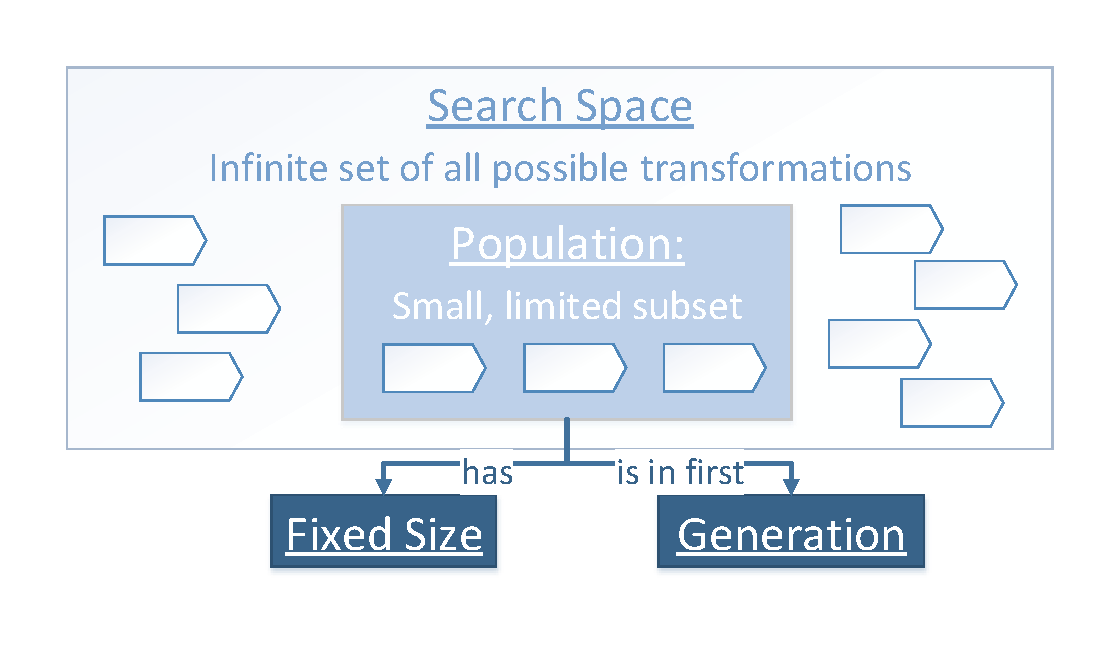
\includegraphics[scale=0.5]{Images/Algorithm_01_PopulationInitialization.pdf} 
	\caption{Population Initialization: The initial \gls{Population} is a small subset of the \gls{SearchSpace} with a fixed size and represents the first generation. Each \gls{Individual} inside is an empty \gls{ModelToModelTransformation}.}
	\label{figAlgorithm_01_PopulationInitialization}
\end{figure}

\textbf{1) Population Initialization}: In the first phase the initial \gls{Population} is created. It represents the first generation with a fixed number of \glspl{Individual}, which are \glspl{ModelToModelTransformation} (see figure \ref{figAlgorithm_01_PopulationInitialization}). Ideally, those are spread across the \gls{SearchSpace}, but as it is infinite this is not feasible. An approximation is to limit the \gls{SearchSpace}, e.g. by a maximum graph size, and by defining a method to spread. Since the approach is pattern based, such a method must be based on those. Applying patterns is equivalent to the application of \glspl{GeneticOperator} within the next execution phases. Hence, the algorithm initializes the \glspl{Individual} with empty \glspl{ModelToModelTransformation}. The bootstrap challenge, which is the issue of not being able to find a proper initial \gls{Population}, is handled by the Mutation Selection Strategies (see section \ref{secMutationSelectionStrategies}). Furthermore, in this phase the size of the \gls{Population} is defined, which will be kept during the execution and therefore is an important factor for the algorithm performance.

\begin{figure}[htb]
	\centering
	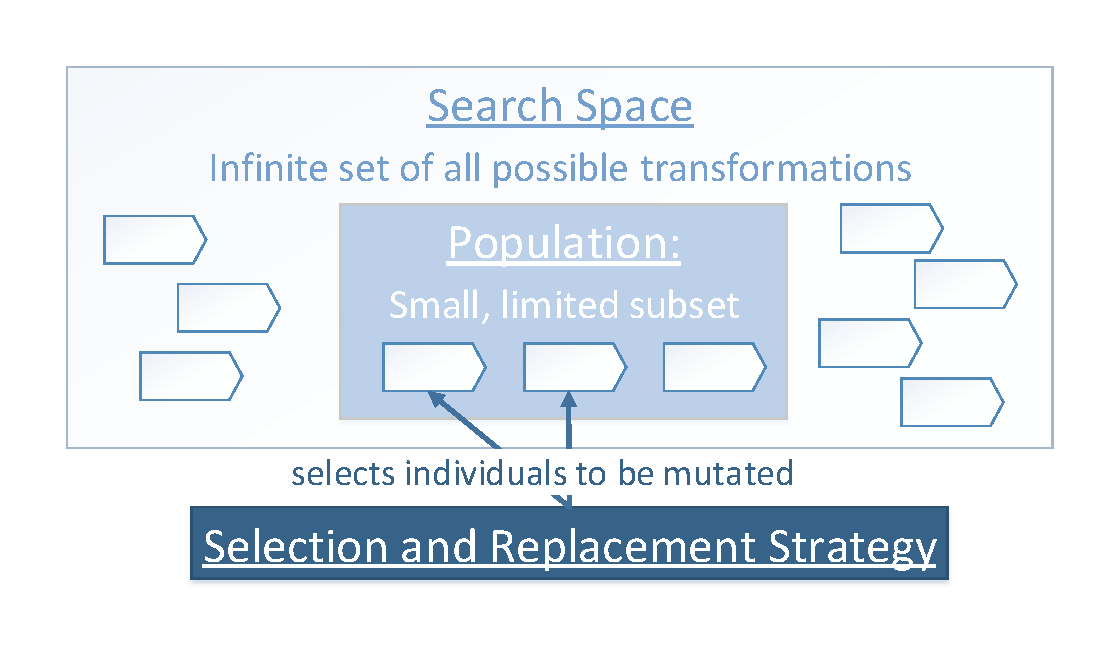
\includegraphics[scale=0.5, trim=0cm 1cm 0cm 1cm, clip=true]{Images/Algorithm_02_Selection.pdf} 
	\caption{Selection: The \gls{SelectionStrategy}, which is part of the Selection and Replacement Strategy, determines \glspl{Individual} in the \gls{Population} that are variated in the next phase.}
	\label{figAlgorithm_02_Selection}
\end{figure}

\textbf{2) Selection}: This phase is the start of the evolution, which requires at first the selection of \glspl{Individual} for the subsequent variation (see figure \ref{figAlgorithm_02_Selection}). The selection alternatives are described in section \ref{secSelectionReplacementStrategies}.

\begin{figure}[htb]
	\centering
	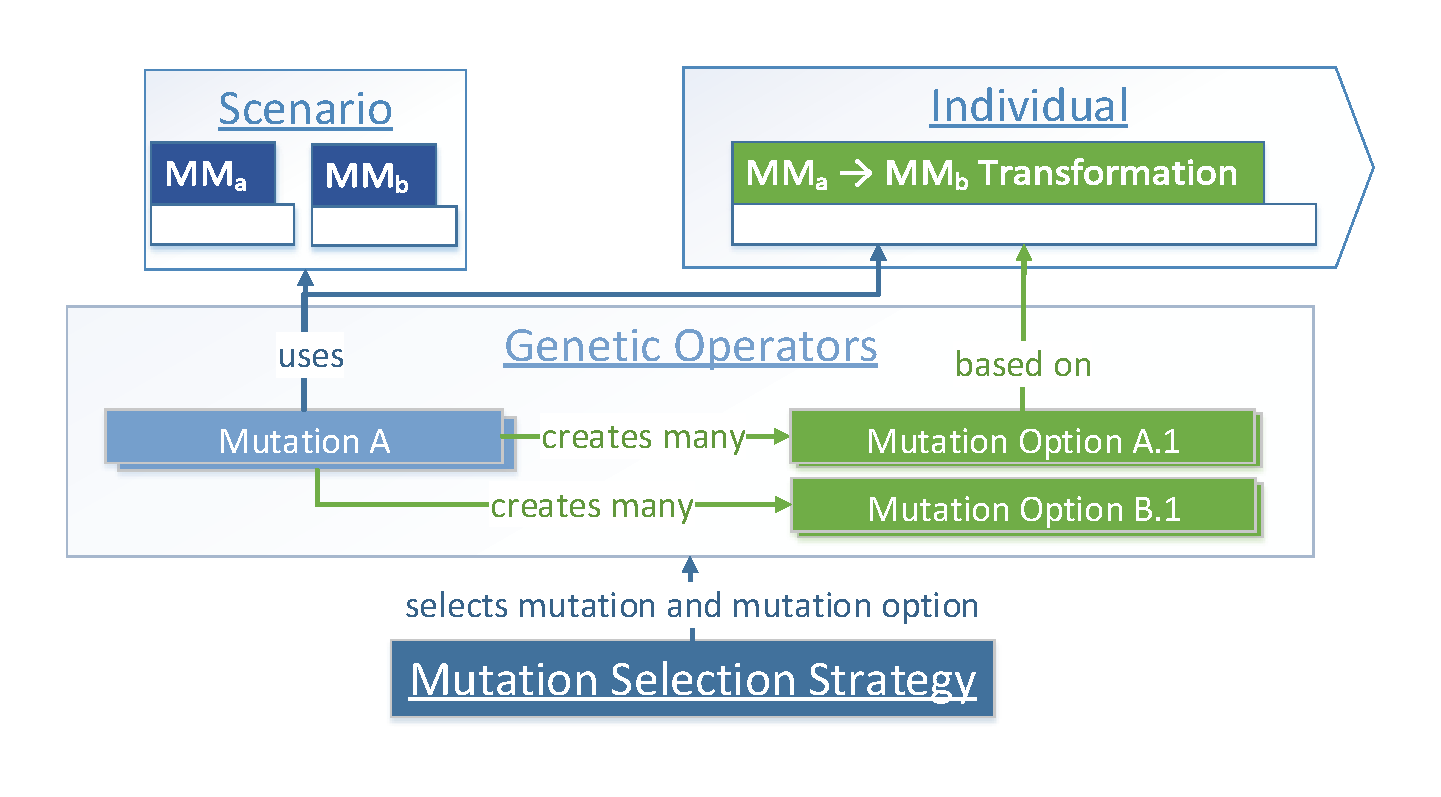
\includegraphics[scale=0.5, trim=0cm 1cm 0cm 1cm, clip=true]{Images/Algorithm_03_Variation_A.pdf} 
	\caption{Variation Step 1: The \glspl{GeneticOperator}, which are all \glspl{Mutation}, use the scenario \glspl{MetaModel} MM$_a$, MM$_b$ and the \gls{ModelToModelTransformation} in the \gls{Individual} to create the context specific mutation options. The Mutation Selection Strategy then selects a \gls{Mutation} and one of the options.}
	\label{figAlgorithm_03_Variation_A}
\end{figure}

\begin{figure}[htb]
	\centering
	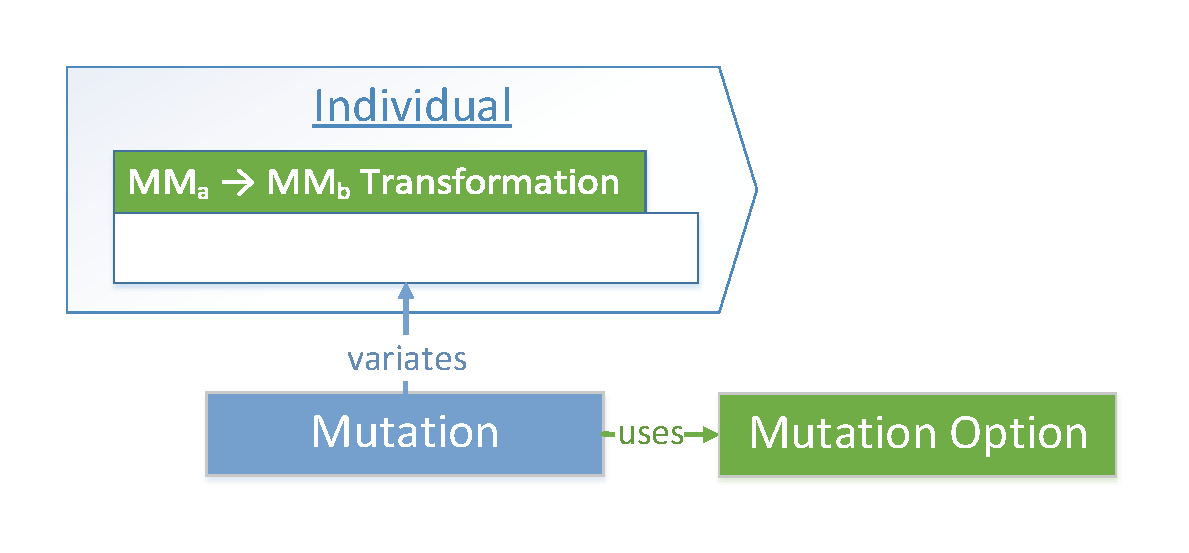
\includegraphics[scale=0.5, trim=0cm 1cm 0cm 1cm, clip=true]{Images/Algorithm_03_Variation_B.pdf} 
	\caption{Variation Step 2: The \gls{Mutation} variates the \gls{ModelToModelTransformation} in the \gls{Individual} using the selected option.}
	\label{figAlgorithm_03_Variation_B}
\end{figure}

\textbf{3) Variation}: As explained in the general design decisions previously in this section, the complexity is tackled by \glspl{GeneticOperator}. They are based on the transformation pattern described in chapter \ref{chapM2MScenarios}. The consequence is that there are multiple operators and each operator has several options in a specific \gls{ModelToModelTransformation}. For example the creation of a \gls{TransformationRule} is an operator. When applied to a transformation of the scenario, where already several rules exist, only the not yet existing ones are such an option. Hence, an option is an instance of a \gls{Mutation}. Furthermore, all operators are \glspl{Mutation} without \glspl{Crossover}, since those are mandatory and were sufficient to solve the scenarios (see chapter \ref{chapEvaluation}). Thus, the first step is to select a \gls{Mutation}, which is described in section \ref{secPatternAndMutations}, and an option using a Mutation Selection Strategy presented in section \ref{secMutationSelectionStrategies} (see figure \ref{figAlgorithm_03_Variation_A}).

The second step is the variation of the \gls{ModelToModelTransformation} with the selected \gls{Mutation} and option (see figure \ref{figAlgorithm_03_Variation_B}).

\begin{figure}[htb]
	\centering
	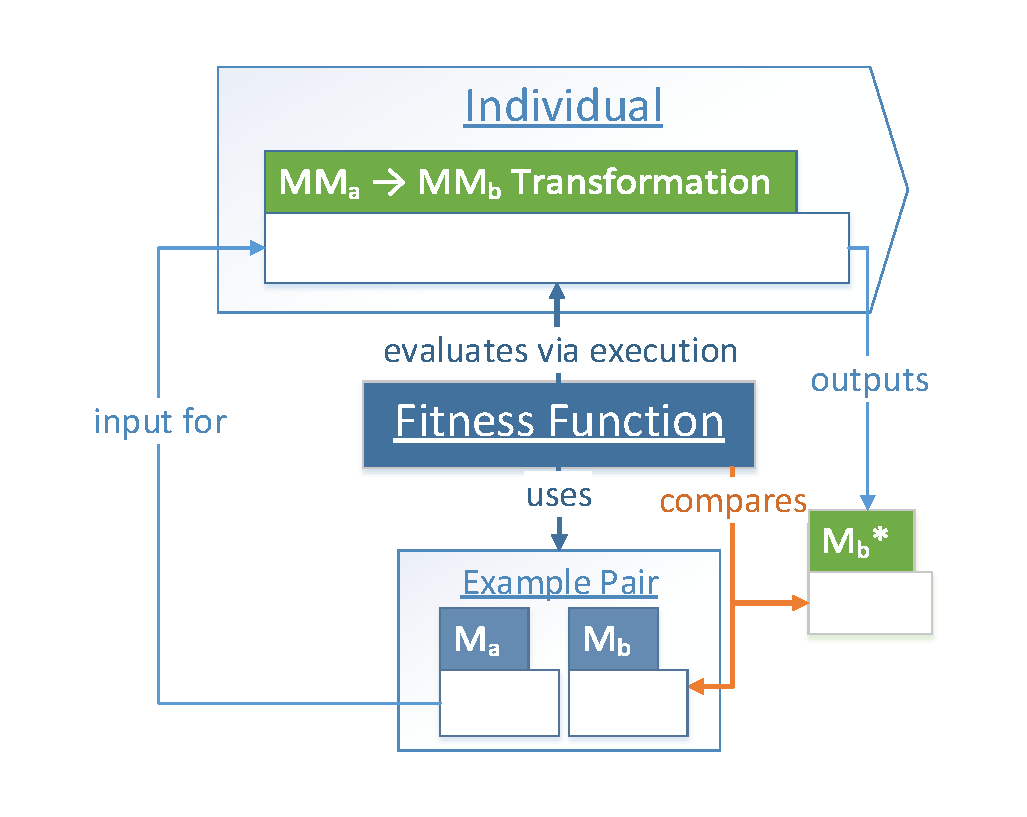
\includegraphics[scale=0.5, trim=0cm 1cm 0cm 1cm, clip=true]{Images/Algorithm_04_FitnessEvaluation.pdf} 
	\caption{Fitness Evaluation: The \gls{FitnessFunction} evaluates the \gls{ModelToModelTransformation} by executing it with the \gls{Model} M$_a$ of the example pair. The resulting \gls{Model} M$_b^*$ is the compared to the example M$_b$.}
	\label{figAlgorithm_04_FitnessEvaluation}
\end{figure}

\textbf{4) Fitness Evaluation}: All variated \glspl{Individual} require an update of the fitness, which is performed in this phase (see figure \ref{figAlgorithm_04_FitnessEvaluation}). The \gls{FitnessFunction} executes the \gls{ModelToModelTransformation} with the \gls{Model} M$_a$ of the example pair. The result M$_b^*$ of this execution is compared with the expected M$_b$ and the differences are then computed into a fitness value. There are several alternatives for the \gls{FitnessFunction} which are described in section \ref{secFitnessFunctions}.

\begin{figure}[htb]
	\centering
	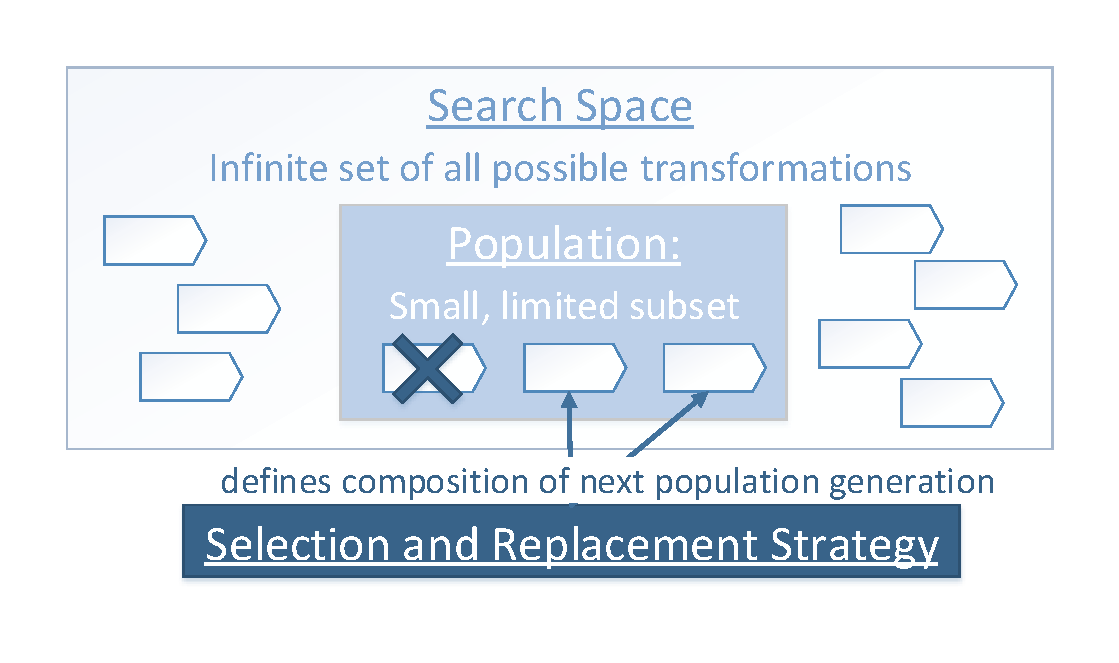
\includegraphics[scale=0.5, trim=0cm 1cm 0cm 1cm, clip=true]{Images/Algorithm_05_Replacement.pdf} 
	\caption{Population Replacement: The \gls{ReplacementStrategy} assembles the next generation of the \gls{Population}}
	\label{figAlgorithm_05_Replacement}
\end{figure}

\textbf{5) Population Replacement}: The last step of the evolutionary cycle is the assembly of the next generation of the \gls{Population} (see figure \ref{figAlgorithm_05_Replacement}). The \gls{ReplacementStrategy}, which is part of the Selection and Replacement Strategy, is applied, whereas the alternatives are described in sub-section \ref{secSelectionReplacementStrategies}.

\textbf{6) Termination}: The algorithm stops in case a transformation is found that produces exactly all the expected M$_b$ \glspl{Model}. Additionally, it stops when a maximum number of \glspl{Generation} is reached. From the solution or \gls{CandidateSolution} with the best fitness, all constructs which do not decrease the fitness are removed. This improves the readability of the \gls{ModelToModelTransformation}.

\newpage
\section{Transformation Pattern, Mutation and Fitness Function Design Method}
\label{secMutationAndFitnessFunctionDesignProcess}

The \gls{ModelToModelTransformation} complexity is primarily handled by the \glspl{Mutation} and also the closely related \gls{FitnessFunction}. Within this thesis, the created \glspl{Mutation} and the \gls{FitnessFunction} were targeted at the simple and complex scenario. Hence, they are not able to solve all possible scenarios. An extension of the algorithm is required for completely different scenarios. This section describes the extension design method in terms of the followed design process.

\begin{figure}[!ht]
	\centering
	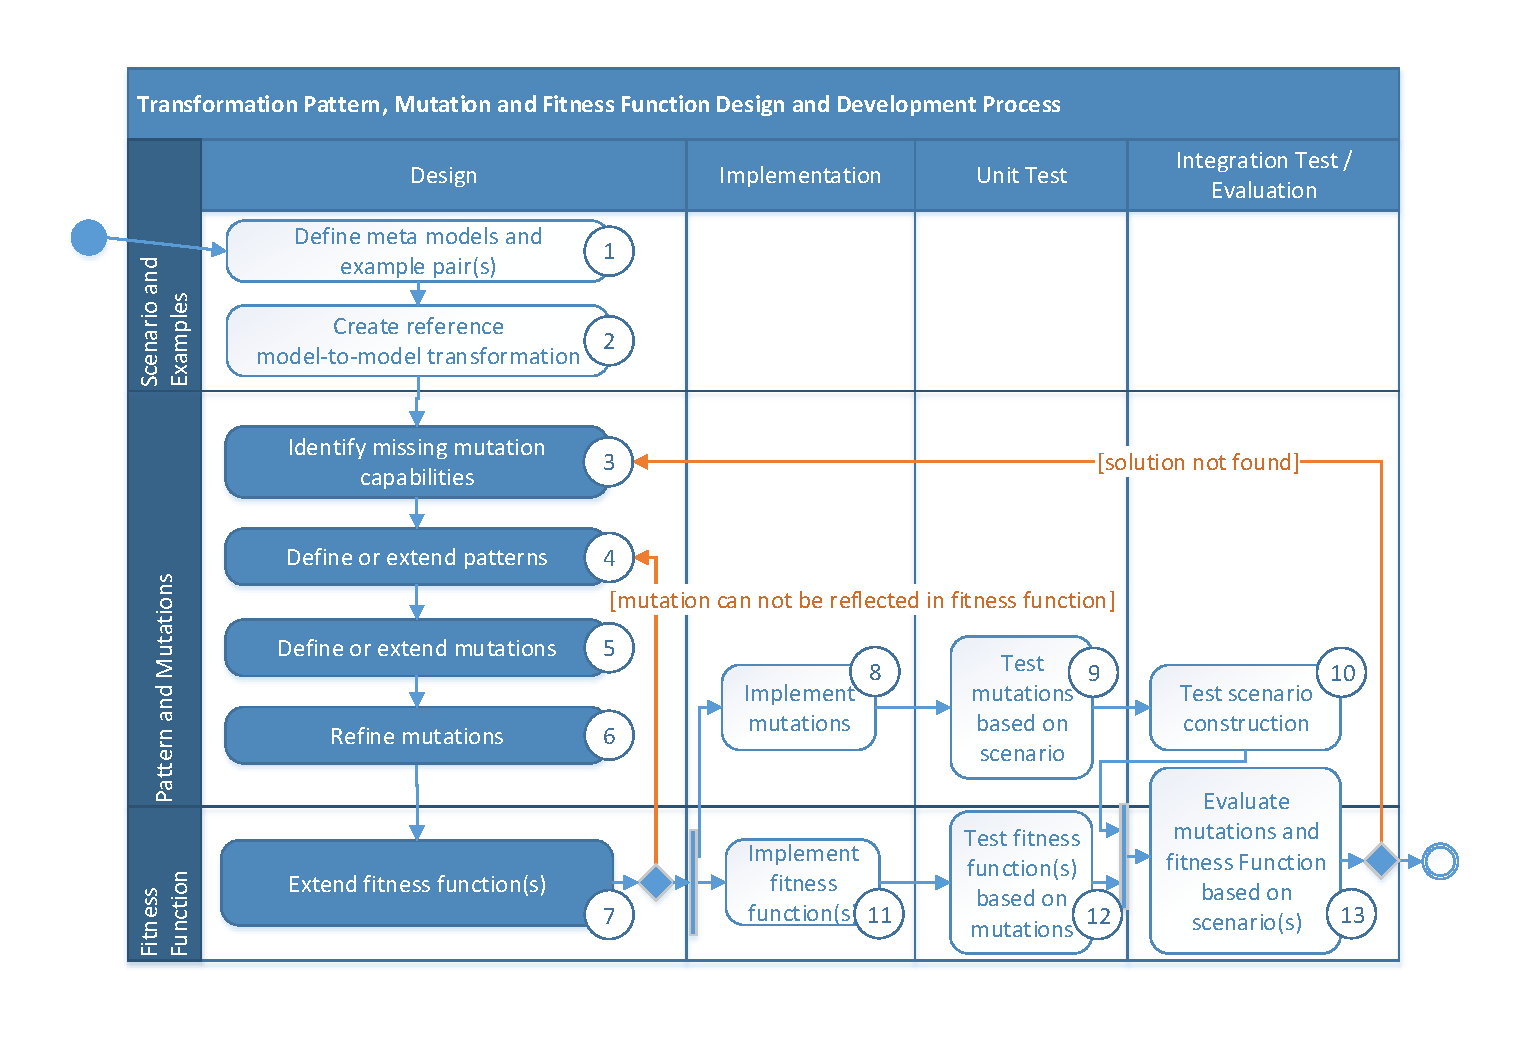
\includegraphics[scale=0.6, trim=0cm 1cm 0cm 1cm, clip=true]{Images/MutationAndFitnessFunctionDevelpomentProcess.pdf} 
	\caption{\Gls{Mutation} and \gls{FitnessFunction} design and development process}
	\label{figMutationAndFitnessFunctionDevelpomentProcess}
\end{figure}

Figure \ref{figMutationAndFitnessFunctionDevelpomentProcess} presents the design process in detail, based on the general process in section \ref{secDesignAndDevelopmentProcess}. The steps 3 to 7 are the main topics within this chapter and therefore highlighted in the overview. The details of step 1 and 2 are explained in chapter \ref{chapM2MScenarios}, while the description of step 8 to 13 is in chapter \ref{chapPrototypeDesign}. In the following paragraphs each step will be described with references to the simple and complex scenario.

\textbf{1) Define source and target \glspl{MetaModel} and example pair(s)}: Since there is no common definition of \glspl{ModelToModelTransformation}, the approach is based on representative scenarios which contain a source and target \gls{MetaModel}. Those are described in chapter \ref{chapM2MScenarios} including the design considerations.

\textbf{2) Create a reference \gls{ModelToModelTransformation}}: The \glspl{MetaModel} of the scenario can be transformed in infinite ways. However, for the desired approach the definition of a desired transformation is required (see figure \ref{figMutationAndFitnessFunctionDesignProcess-Step2}). This is the foundation for the identification of the necessary \glspl{Mutation}. Since the result produced by the algorithm is not always complete, the created transformations should be comprehensible by humans. Thus, the design goal is not a transformation which could be automatically created easily, but which is readable.

\begin{figure}[!ht]
	\centering
	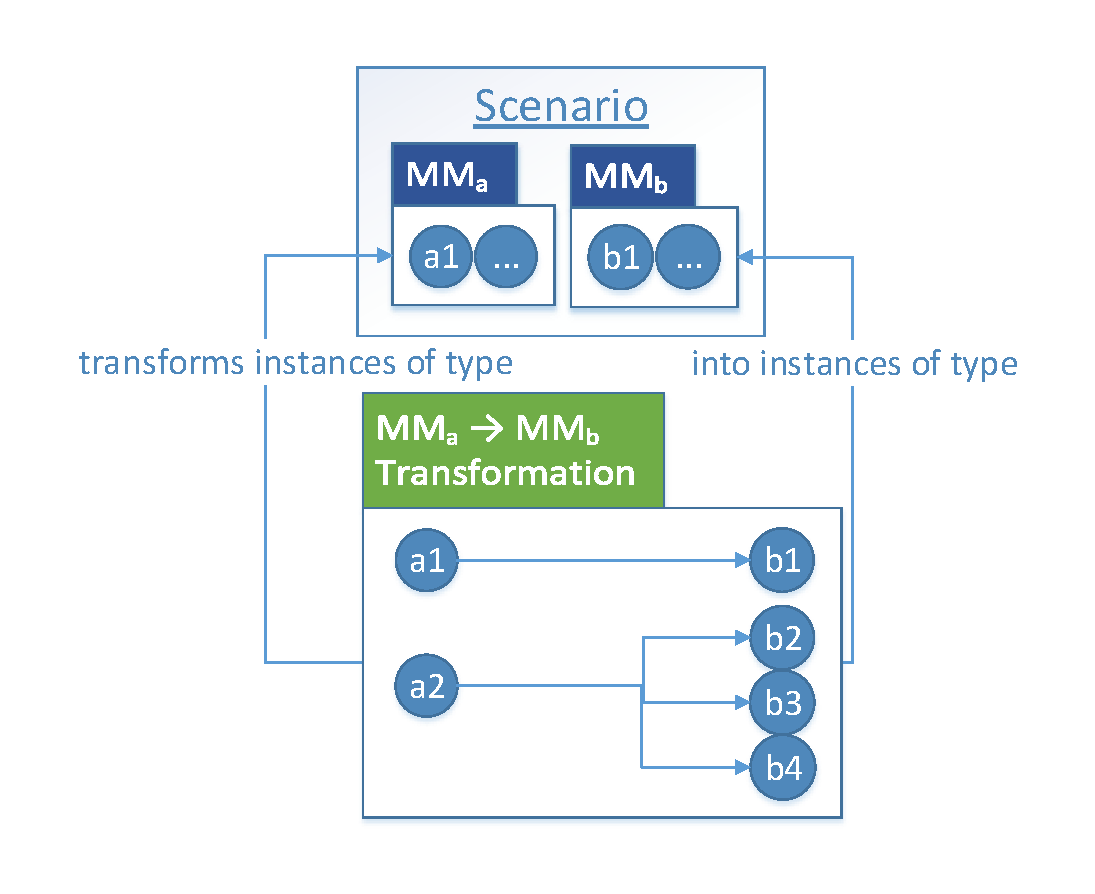
\includegraphics[scale=0.5, trim=0cm 1cm 0cm 1cm, clip=true]{Images/MutationAndFitnessFunctionDesignProcess-Step2.pdf} 
	\caption{\Gls{Mutation} and \gls{FitnessFunction} design and development process - Step 2: Create a reference \gls{ModelToModelTransformation}}
	\label{figMutationAndFitnessFunctionDesignProcess-Step2}
\end{figure}


\textbf{3) Identify missing \gls{Mutation} capabilities}: In the case the scenario is not solvable with the given \glspl{Mutation}, the \gls{ModelToModelTransformation} will be inspected and the missing aspects highlighted (see figure \ref{figMutationAndFitnessFunctionDesignProcess-Step3}). 

The following example starts after the algorithm supports the simple scenario. Listing \ref{lstETLFragementOfComplexExample} shows a small fragment of the complex scenario showing the one-to-many rule that creates for a single outgoing transitions of a complex state, multiple transitions each starting at one of the inner states. The rule contains a loop which iterates over those states, creates a transition and adds this transition to the result list. Since the simple example does not require any of the mentioned aspects, none of those are supported.

\begin{lstlisting}[language=ETL,caption={Fragment of Complex State Machine to Simple State Machine \gls{ModelToModelTransformation} in \gls{ConcreteSyntax} of \Gls{EpsilonTransformationLanguage}},label={lstETLFragementOfComplexExample}]
rule TransitionFromComplexStateToManyTransitions
	transform sourceTransition : Source!Transition
	to targetTransitions : Sequence(Target!Transition) {
	...
	for(sourceState in sourceTransition.Source.States) {
		var targetTransition = new Target!Transition;
		targetTransitions.add(targetTransition);
		...
	}
}
\end{lstlisting}

\begin{figure}[!ht]
	\centering
	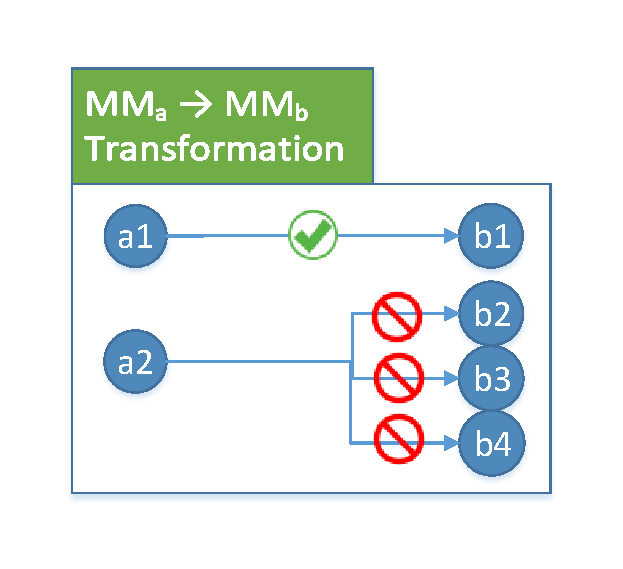
\includegraphics[scale=0.5, trim=0cm 1cm 0cm 1cm, clip=true]{Images/MutationAndFitnessFunctionDesignProcess-Step3.pdf} 
	\caption{\Gls{Mutation} and \gls{FitnessFunction} design and development process - step 3: Identify missing \gls{Mutation} capabilities}
	\label{figMutationAndFitnessFunctionDesignProcess-Step3}
\end{figure}


\textbf{4) Define or extend patterns}: The missing aspects, resulting from the previous step, have to be arranged into transformation patterns. Hence, the main task is to create or extend the set of transformation patterns (see figure \ref{figMutationAndFitnessFunctionDesignProcess-Step4}). The challenge is to create patterns that are not only tailored for the current scenario, but are also not too generic and thereby difficult to be captured by the \gls{FitnessFunction} in step 7. This is therefore the most important design step. 

Proceeding with the example presented in the previous step in listing \ref{lstETLFragementOfComplexExample}, this results in the following consideration: The whole loop structure is not yet included in any pattern. Thus, a pattern might create loop structures using some enumerable \gls{Property} from the ``sourceTransition" or ``targetTransition". This does not result in a different output M$_b^*$. Hence, this renders a measurement of any change in the output M$_b^*$ impossible in step 7. The pattern needs to be more coarse grained. In this case, the intention of the loop is to create multiple \glspl{Object} in the target \gls{Model} M$_b$ for a single one in the source. Using this information the pattern is ``One-to-Many" on M2 level with some restrictions regarding the enumerable resulting in the ``Many" \glspl{Object}. Figure \ref{figTransformationPattern_OneToManyObjectsOfSameType} shows this pattern, which is explained in section \ref{secPatternAndMutations}.

\begin{figure}[!ht]
	\centering
	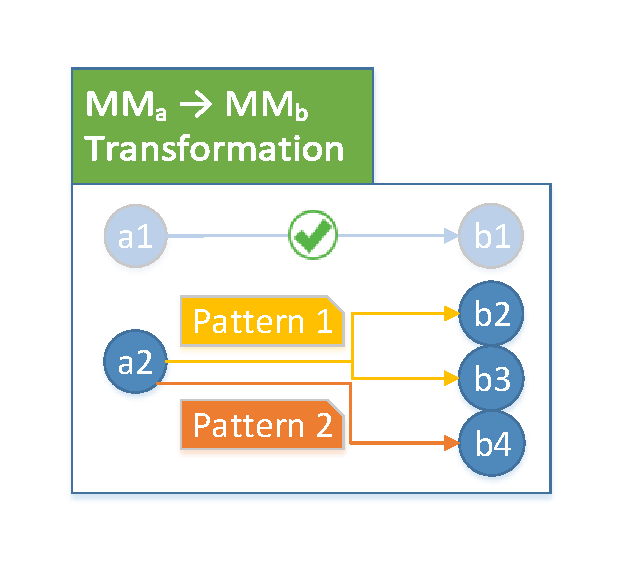
\includegraphics[scale=0.5, trim=0cm 1cm 0cm 1cm, clip=true]{Images/MutationAndFitnessFunctionDesignProcess-Step4.pdf} 
	\caption{\Gls{Mutation} and \gls{FitnessFunction} design and development process - step 4: Define or extend patterns}
	\label{figMutationAndFitnessFunctionDesignProcess-Step4}
\end{figure}


\begin{figure}[!ht]
	\centering
	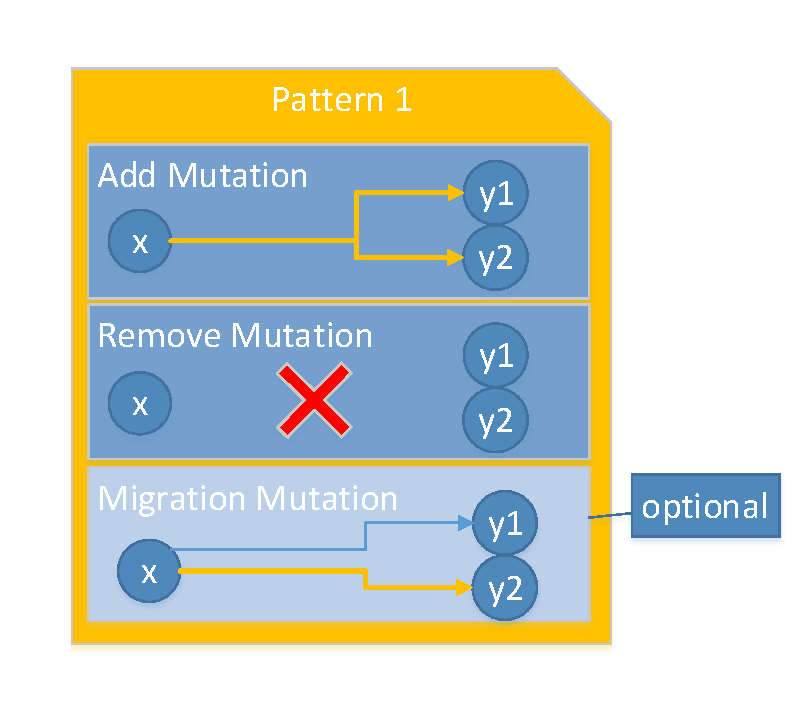
\includegraphics[scale=0.5, trim=0cm 1cm 0cm 1cm, clip=true]{Images/MutationAndFitnessFunctionDesignProcess-Step5.pdf} 
	\caption{\Gls{Mutation} and \gls{FitnessFunction} design and development process - Step 5: Define or extend \glspl{Mutation}}
	\label{figMutationAndFitnessFunctionDesignProcess-Step5}
\end{figure}

\textbf{5) Define or extend \glspl{Mutation}}: Using the pattern, the next step is to derive the actual \glspl{Mutation} (see figure \ref{figMutationAndFitnessFunctionDesignProcess-Step5}). Those are the tools of the algorithm to move through the \gls{SearchSpace}. In order to provide the algorithm the minimal ability to move back and forth, at least an add- and remove-\gls{Mutation} are required. Beyond this also more fine-grained \glspl{Mutation} are possible that enable the algorithm to make more precise moves. A \gls{Mutation} can also be associated to multiple patterns, especially remove-\glspl{Mutation}. The approach contains only a single one to remove a whole transformation rule. Since all everything else is contained in rules, this is sufficient.

Based on the example the add-\gls{Mutation} creates a transformation rule with the loop that iterates over an enumerable \gls{Property}. The remove-\gls{Mutation} is realized through the transformation rule removal \gls{Mutation}.

\begin{figure}[!ht]
	\centering
	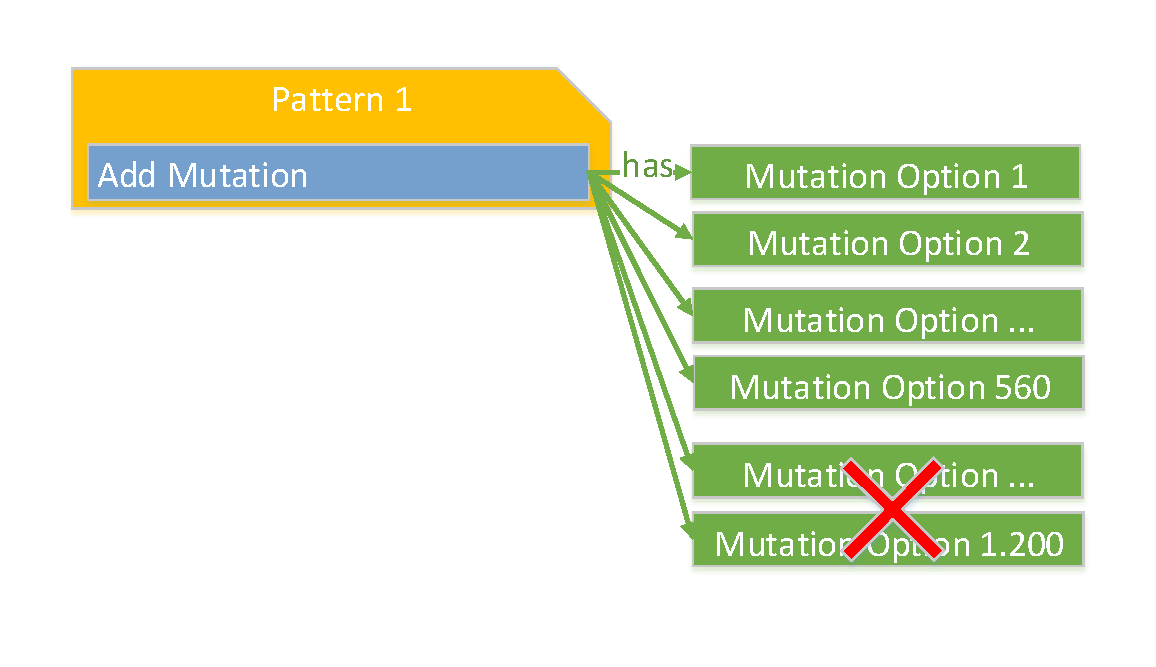
\includegraphics[scale=0.5, trim=0cm 1cm 0cm 1cm, clip=true]{Images/MutationAndFitnessFunctionDesignProcess-Step6.pdf} 
	\caption{\Gls{Mutation} and \gls{FitnessFunction} design and development process - step 6: Refine mutations}
	\label{figMutationAndFitnessFunctionDesignProcess-Step6}
\end{figure}

\textbf{6) Refine \glspl{Mutation}}: Applying the created \glspl{Mutation} in a specific context usually creates too many possible options (see figure \ref{figMutationAndFitnessFunctionDesignProcess-Step6}). The task in this step is to identify and remove options that either result in erroneous \glspl{ModelToModelTransformation} or are difficult to handle in the \gls{FitnessFunction}. Thereby, the \gls{EvolutionaryAlgorithm} less likely ends up in an unguided trial-and-error situation.

Applying the ``One-to-Many" pattern of the running example to a \gls{ModelToModelTransformation}, results in a large number of options because of the following two parameters explained. First, depending on the \glspl{MetaModel} MM$_a$ and MM$_b$, there are several possible relations of MM$_a$-MM$_b$ \glspl{Class}. Second, the possibilities for the ``Many" source are gathered by analyzing the \glspl{Property} and sub-\glspl{Property} of the MM$_a$-\gls{Class}. With this information the analysis for possible restrictions starts. The first part covering the relations of MM$_a$-MM$_b$ \glspl{Class} cannot be further reduced, but the second one can be.

Since there are several issues, only three are explained. The analysis of \glspl{Property} and sub-\glspl{Property} causes a lot of options depending on the \gls{MetaModel}. Assuming that a \gls{Property} chain like ``a.b.c.d.e" and ``a.b.c.d.f" exist. Both are enumerable \glspl{Property}, but none of them is the one which is required to create the required \glspl{Object}. Thus, the \gls{FitnessFunction} cannot distinguish between them. This is the first issue. A lot of those kind of chains are likely to exists, since in the complex scenario only one results in a valid solution. In order to avoid such a random search, an assumption about the maximum depth of the chain is added to refine the ``One-to-Many" pattern. In this context the analyzed \gls{Property} chains are of depth two, which is the minimum required to solve the given scenario.

The second issue is the possibility for self-references in the transformation rule through the enumerated \gls{Property}, which renders the whole \gls{ModelToModelTransformation} defective, since the execution cannot stop. Those options are also removed to avoid this situation.

Finally, the third issue is the one of contradictory transformations. In a situation where A is transformed into B, but at the same time A should be equivalent to C, the output is a corrupted \gls{Model} M$_b^*$. Furthermore, the manual analysis of the resulting transformation becomes difficult, hence this has to be avoided, too.

\textbf{7) Extend \glspl{FitnessFunction}}: While the \glspl{Mutation} enable the algorithm to move through the \gls{SearchSpace}, the \gls{FitnessFunction} is responsible for the guidance by rating each move. Therefore, each change of a \gls{Mutation} should be measurable by the \gls{FitnessFunction}. Ideally, a small change of a \gls{Mutation} should also cause only a small change in the result of the \gls{FitnessFunction} (see sub-section \ref{secEvolutionaryAlgorithms}). Since creating any change in the output is already difficult within the large \gls{SearchSpace} created by the \gls{TransformationLanguage}, this requirement is not applied.

%The \gls{FitnessFunction} execution has two phases. At first the comparison of the \glspl{Model} M$_b$ and M$_b^*$ results in a list of differences. Thereafter the rating of those result in a fitness value between 0 and 100 (see section \ref{secAlgorithmOverview}). Since there are several options for both, multiple \glspl{FitnessFunction} have been designed (see section \ref{secFitnessFunctions}) and evaluated (see chapter \ref{chapEvaluation}) in order to identify the differences. Adding a measurement for a \gls{Mutation} therefore requires an update of all of them.

As mentioned in step 6, the main issue dealt with in this step, is that a large fraction of the options of a \gls{Mutation} often leads to no difference in the fitness. Since the scope of the \gls{FitnessFunction} is limited to the output, there is often no possibility to change the function. If this is the case, the development needs to start over at step 4 and consider a different pattern structure, different \glspl{Mutation} or additional refinements of the \glspl{Mutation}.

\textbf{8) Implement \glspl{Mutation}}: The realization of the \glspl{Mutation} is explained in sub-section \ref{secRealizationOfMutations}.

\textbf{9) Test \glspl{Mutation} based on scenario}: Testing \glspl{Mutation} individually is important because the more are involved, the more difficult is the analysis of issues. The test of a \gls{Mutation} is based on parts of the scenarios. Thus, for each \gls{Mutation} a small test case with a \glspl{ModelToModelTransformation} as an input and output has to be created.

\begin{figure}[!ht]
	\centering
	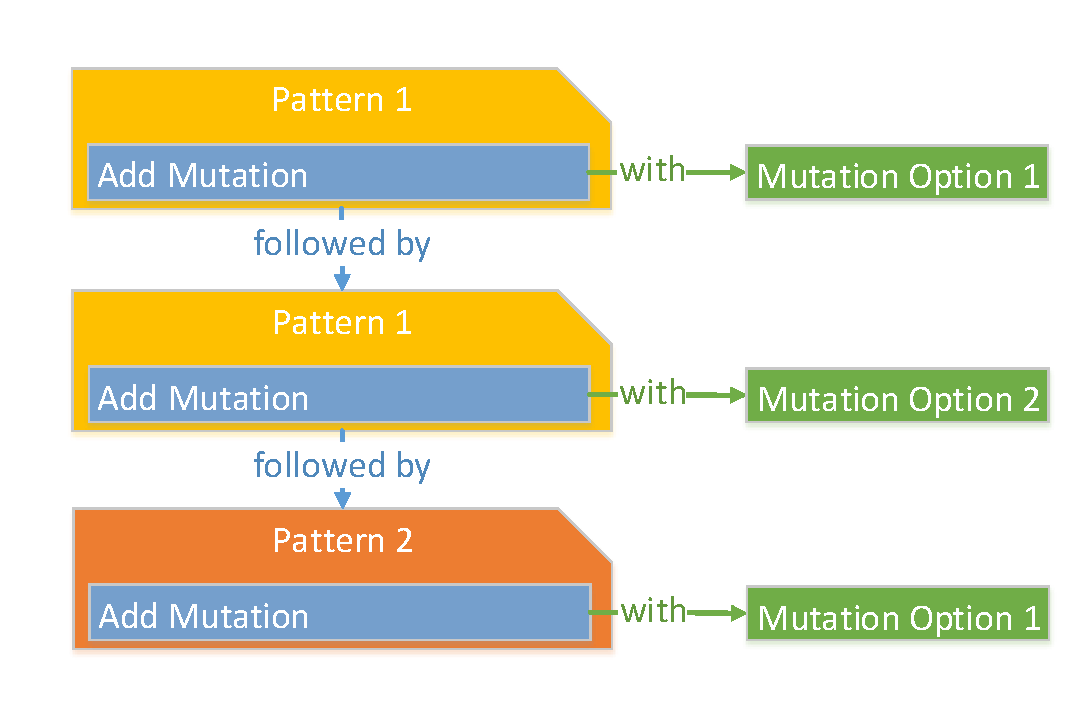
\includegraphics[scale=0.5, trim=0cm 1cm 0cm 1cm, clip=true]{Images/MutationAndFitnessFunctionDesignProcess-Step10.pdf} 
	\caption{\Gls{Mutation} and \gls{FitnessFunction} design and development process - Step 10: Test scenario construction}
	\label{figMutationAndFitnessFunctionDesignProcess-Step10}
\end{figure}

\textbf{10) Test scenario construction}: In order to ensure that the \glspl{Mutation} are able to construct the whole scenario, an integration test is required. This test is using specific \gls{Mutation} options, which represent one possibility to construct the output (see figure \ref{figMutationAndFitnessFunctionDesignProcess-Step10}). Thereby, further analysis in the evaluation phase can be simplified.

\textbf{11) Implement \glspl{FitnessFunction}}: The realization of \glspl{FitnessFunction} is explained in chapter \ref{chapPrototypeDesign}.

\textbf{12) Test \glspl{FitnessFunction} based on \glspl{Mutation}}: The \glspl{FitnessFunction} need to be tested individually based on defined scenarios. Since a complete test is difficult, only corner cases are verified. During the evaluation in the next step, control samples are be collected and added as test cases.

\textbf{13) Evaluate \glspl{Mutation} and \glspl{FitnessFunction} based on scenario(s)}: In the final step, all entities are assembled in order to verify at first that the algorithm is able to find at least any solution. Afterwards, the evaluation is started to compare and analyze the entities (see chapter \ref{chapEvaluation}). This step might also identify issues which require to re-consider the design.

For example the algorithm behaves in the first generations like a brute-force algorithm, because the \glspl{FitnessFunction} requires an identical ``Name" \gls{Property} to find an \gls{Object} match. Hence, the algorithm at first has to find the right ``Name", until any further \glspl{Association} or \glspl{Property} can be analyzed, thus ending in a situation, where only a single \gls{Mutation} option can improve the fitness. To avoid this situation a heuristic \gls{Object} comparison is added (see section \ref{secFitnessFunctions}).

\section{Transformation Pattern and Mutations}
\label{secPatternAndMutations}

\begin{figure}[htb]
	\centering
	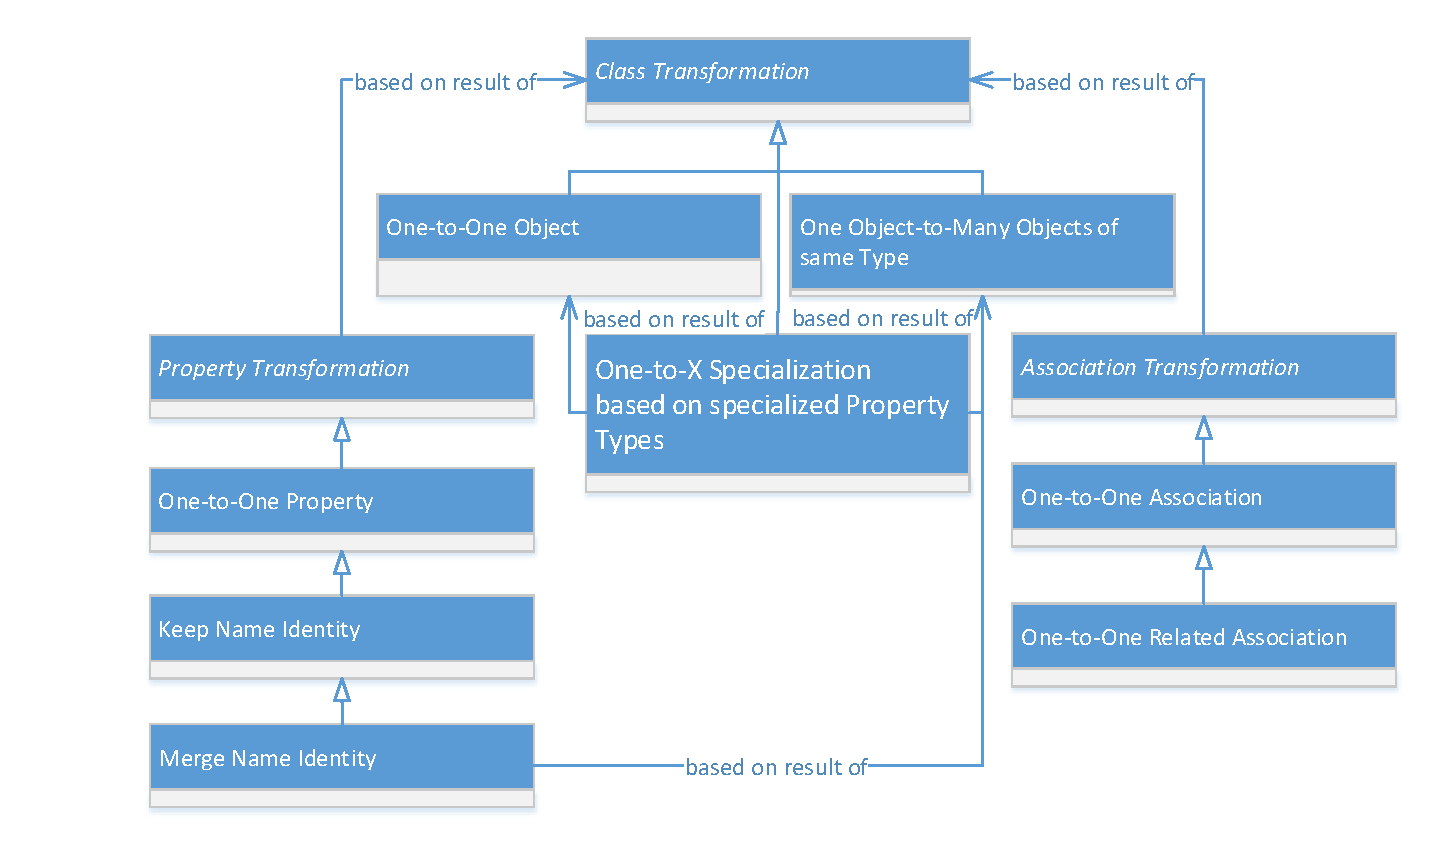
\includegraphics[scale=0.6, trim=0cm 0cm 0cm 0cm, clip=true]{Images/TransformationPattern_Overview.pdf} 
	\caption{Transformation Pattern Overview}
	\label{figTransformationPattern_Overview}
\end{figure}

In this section, the transformation pattern and the \glspl{Mutation} are presented. They are required to solve the simple and complex transformation scenario. An overview is provided in figure \ref{figTransformationPattern_Overview}. The pattern structure is derived from the conclusions of sub-section \ref{secTransformationComplexity} and the construction of the scenarios in chapter \ref{chapM2MScenarios}. The general pattern categories are \Gls{Class} Transformation, \Gls{Property} Transformation and \Gls{Association} Transformation according to the identified connect-able \glspl{Class} in the simplified \gls{MetaObjectFacility}. The pattern in these categories are described in the following subsections and have been developed according to the process described in the previous section.

As explained in the previous section, for each pattern at least an add- and one remove-\gls{Mutation} is required. The transformation pattern represents also the add-\gls{Mutation} unless otherwise stated. Since the remove-\gls{Mutation} can be coarse grained, only a single one exists which removes a whole transformation rule with all contained transformations.

\subsection{Class Transformation}
\label{secClassTransformation}

\begin{figure}[!ht]
	\centering
	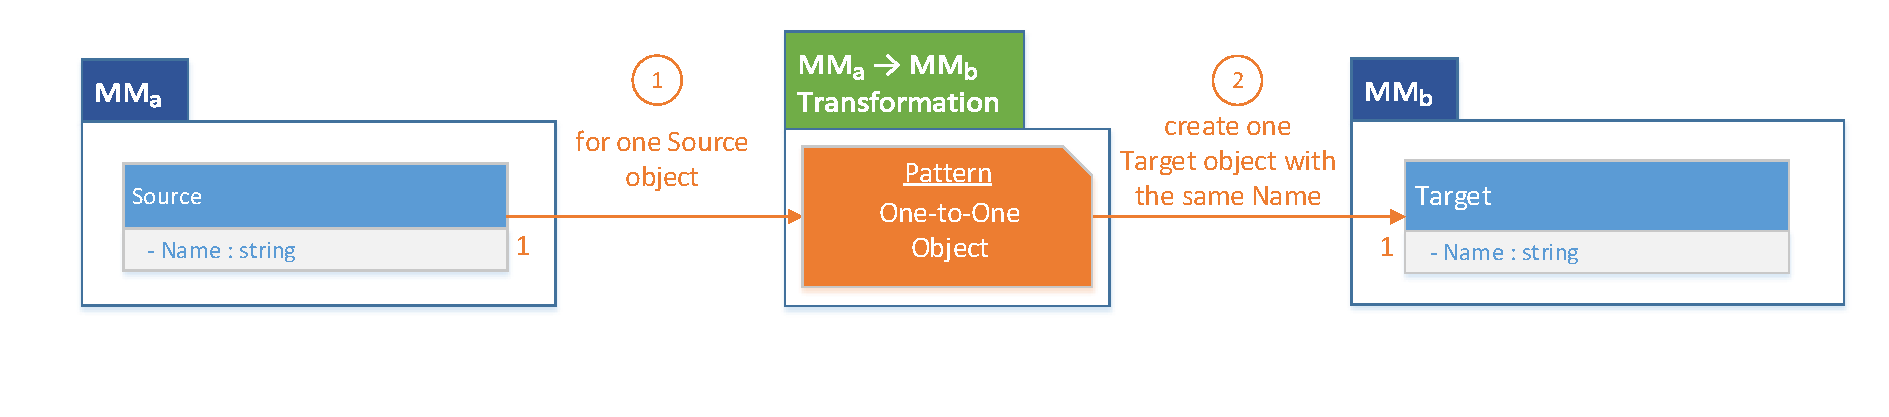
\includegraphics[scale=0.48, trim=0cm 1cm 0cm 0cm, clip=true]{Images/TransformationPattern_OneToOneObjectOfSameType.pdf} 
	\caption{Transformation Pattern: One-to-One Object}
	\label{figTransformationPattern_OneToOneObjectOfSameType}
\end{figure}

\textbf{One-to-One Object}: This is a simple, fundamental pattern required in both scenarios, which describes the transformation of one \gls{Object} of type Source from MM$_a$ into one \gls{Object} of type Target from MM$_b$ (see figure \ref{figTransformationPattern_OneToOneObjectOfSameType}). Additionally, the ``Name" \gls{Property} value is preserved. This ensures that \glspl{FitnessFunction} relying on an identical ``Name", are able to measure a difference in the output without any further \gls{Mutation}.
% - Add + Replace?: AddRuleWithNameMapping
%- Remove: RemoveRule

\begin{figure}[!ht]
	\centering
	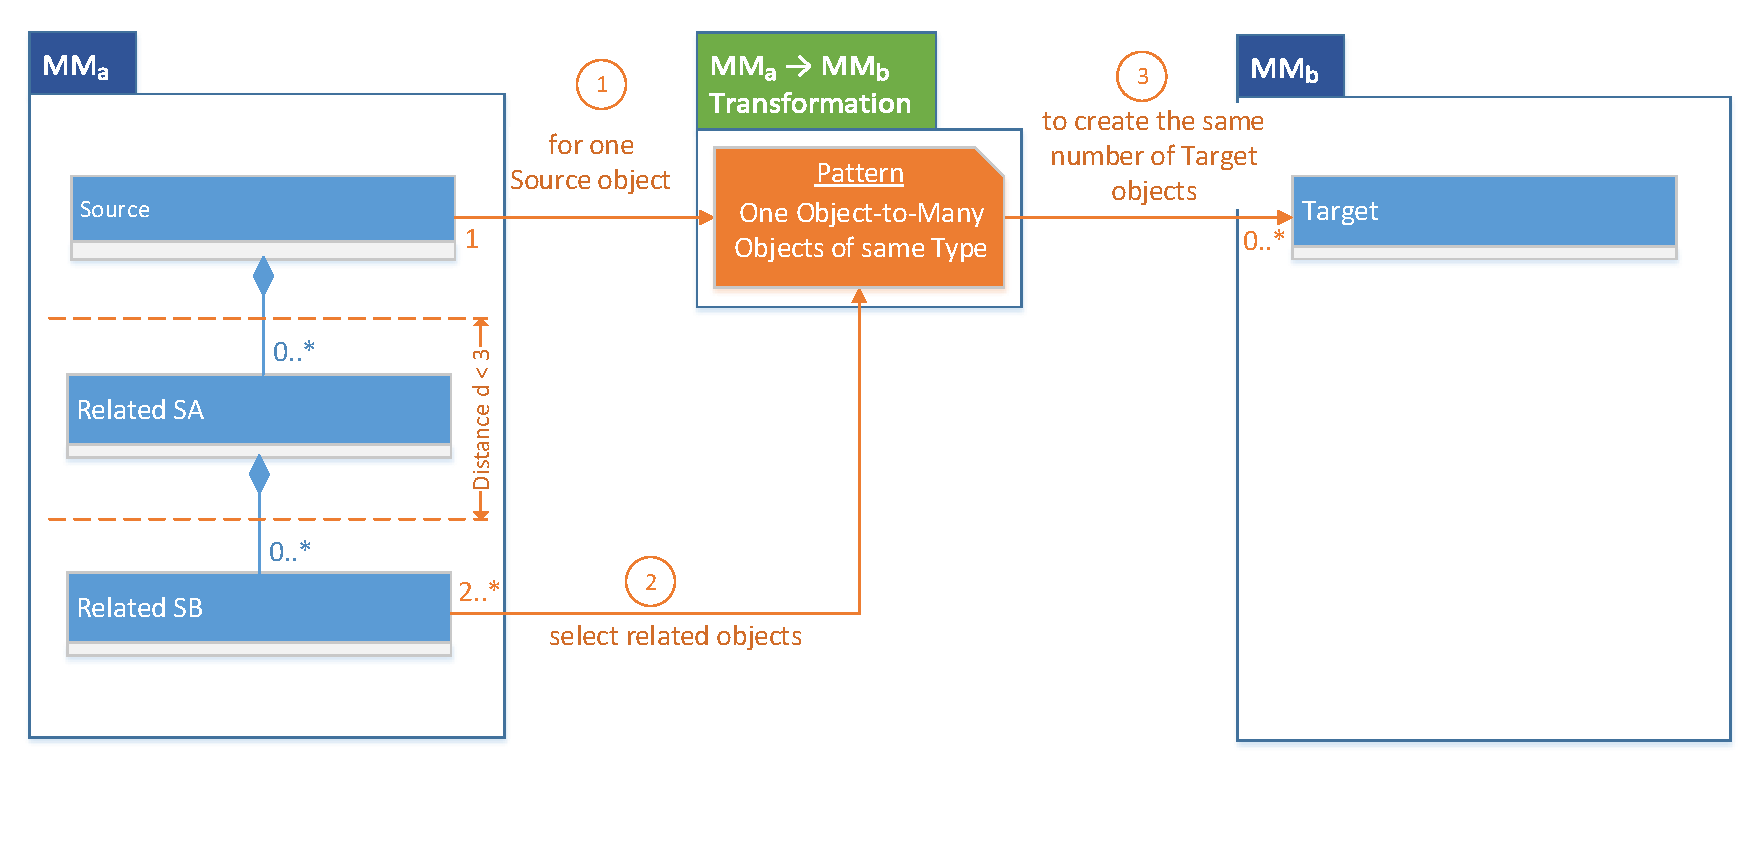
\includegraphics[scale=0.48, trim=0cm 1cm 0cm 0cm, clip=true]{Images/TransformationPattern_OneToManyObjectsOfSameType.pdf} 
	\caption{Transformation Pattern: One Object-to-Many Objects of same Type}
	\label{figTransformationPattern_OneToManyObjectsOfSameType}
\end{figure}
 
\textbf{One Object-to-Many Objects of same Type}: Transforming one \gls{Object} of type Source from MM$_a$ into several \glspl{Object} of type Target from MM$_b$ is required in the complex scenario for the outgoing transitions of a complex state which is shown in figure \ref{figTransformationPattern_OneToManyObjectsOfSameType} (see section \ref{secM2MScenarioBehavioralComplex}). In general, there are several possible sources, which define how many \glspl{Object} are created. For example, this could be defined in a \gls{Property}, calculated based on \glspl{Property}, a fixed number etc. In order to solve the complex scenario where the number of required transitions is the number of inner states, the pattern uses related \glspl{Object}. Those can be directly or indirectly related to the Source type. Since this results in a large number of options, the distance is restricted to be less than three \glspl{Association} in a row. This is the minimum number required in the complex scenario.
%  - Add: AddRuleOneToManyOfSameKind
  
\begin{figure}[!ht]
	\centering
	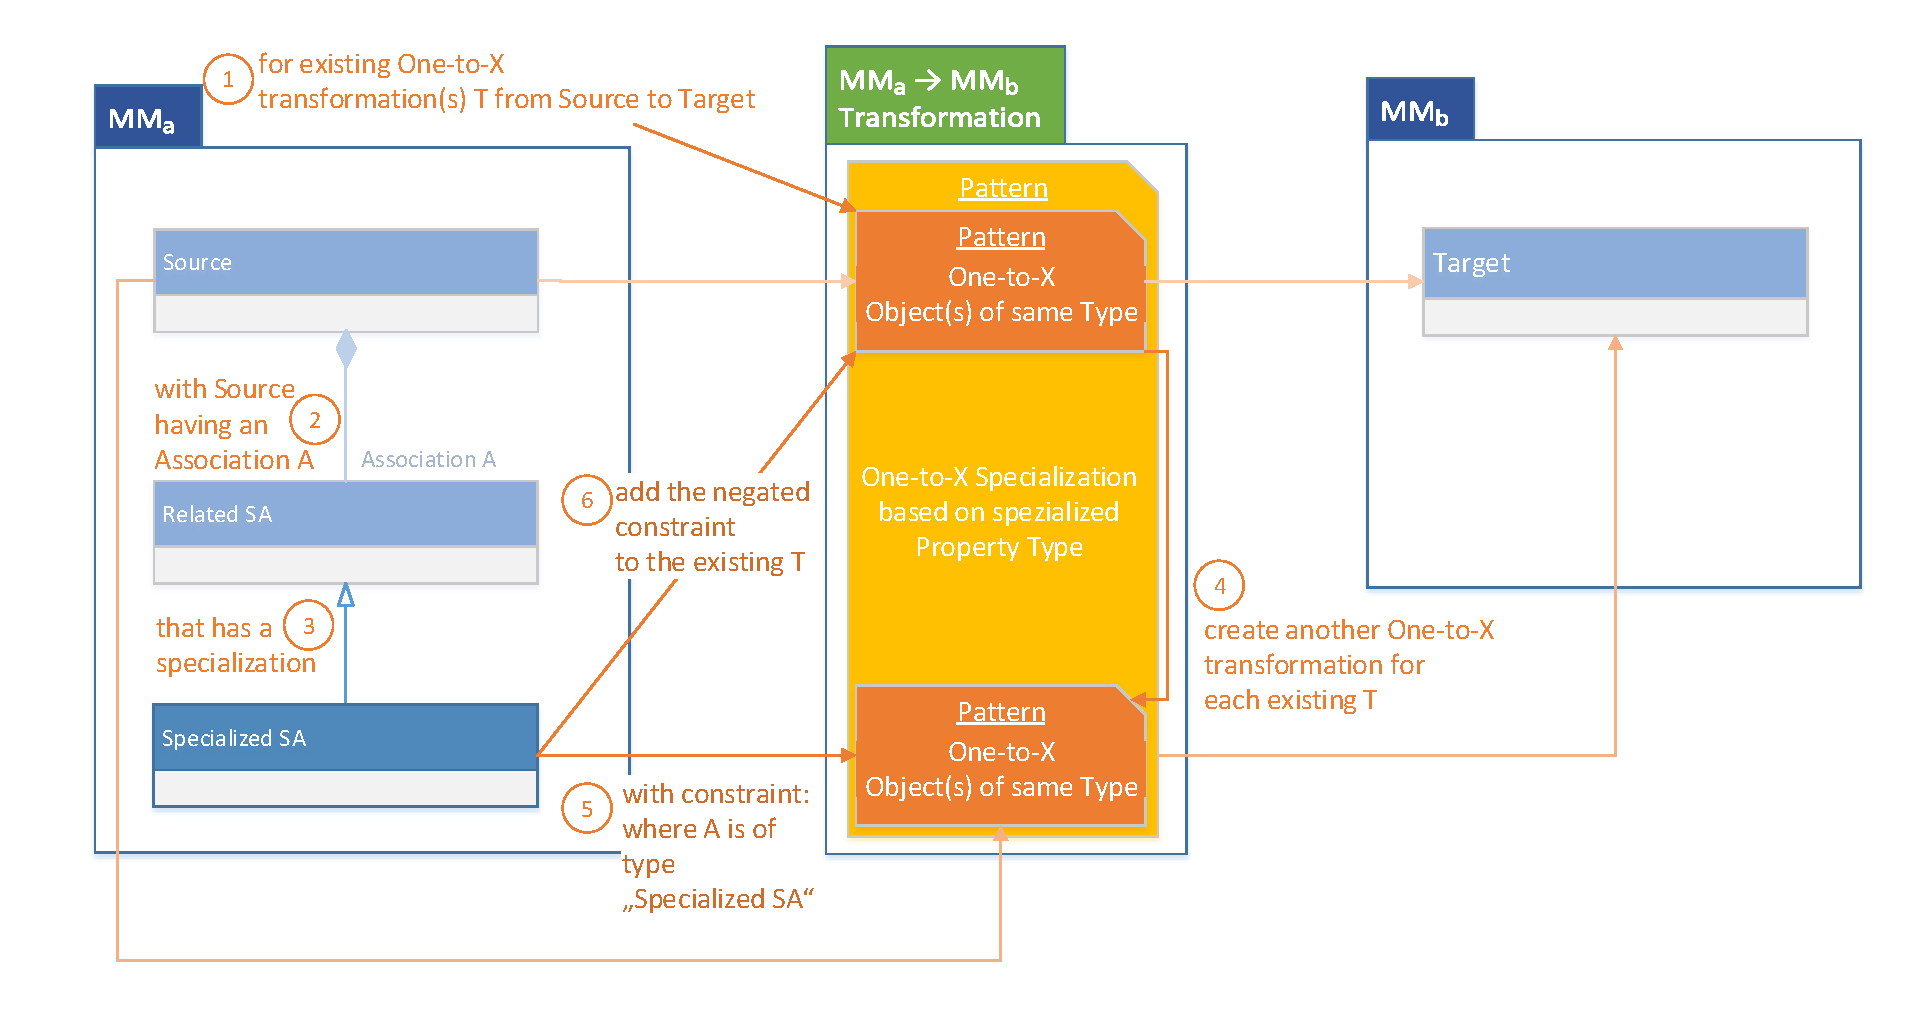
\includegraphics[scale=0.48, trim=0cm 0cm 0cm 0cm, clip=true]{Images/TransformationPattern_OneToXSpecializationBasedOnSpecializedPropertyTypes.pdf} 
	\caption{Transformation Pattern: One-to-X Specialization based on specialized Property Types}
	\label{figTransformationPattern_OneToXSpecializationBasedOnSpecializedPropertyTypes}
\end{figure} 
 
\textbf{One-to-X Specialization based on specialized Property Types}: The reference transformation for the complex scenario defines multiple Transition \glspl{TransformationRule}, depending on the context which resulted in this pattern (see section \ref{secM2MScenarioBehavioralComplex}). Using this pattern the algorithm is able to start with one of those. Afterwards, the algorithm can add the other Transition transformations step-by-step using an add-\gls{Mutation} option of this pattern. Thereby, the relevant context of a Transition is the type of the associated States. Those can be only a State or a Composite State, while the latter is a specialization of the former. For example a Transition starting at a State and ending at a Composite State has to be transformed into a Transition ending at the former Initial State of the Composite State. In the following the pattern is described in detail.

The derived concept is to take an existing \gls{TransformationRule} defined by a transformation pattern, which is cloned. Both of them are then constrained with the opposite condition. This is the foundation to achieve context specific transformations for a single type (see figure \ref{figTransformationPattern_OneToXSpecializationBasedOnSpecializedPropertyTypes}).

The pattern creates an additional transformation for the same type. Since there might be more than one context restriction, there could be also more than one existing transformation for a type. Therefore, this pattern assumes that there is a set of existing transformations which are all cloned. The second aspect is the definition of the constraint. In general, there are infinite sources for such a constraint, e.g. a \gls{Property} value or an optional \gls{Association}. In order to be able so solve the complex scenario according to the reference transformation, the derived concept is based on inheritance. Transitions in the scenario relate States, which can be Composite States since this is a sub-type. Hence, the pattern analyses the inheritance structure of the associated \glspl{Class} of type Source in MM$_a$ in a distance less than three as in the previous pattern. Whenever there is an inheritance, this is a possible constraint and thus considered as a \gls{Mutation} option.

%  - Add: SplitRuleAndAddGuardsForSuperclasses
% - Remove: RemoveRule
  
\subsection{Property Transformation} 
  
\begin{figure}[!ht]
	\centering
	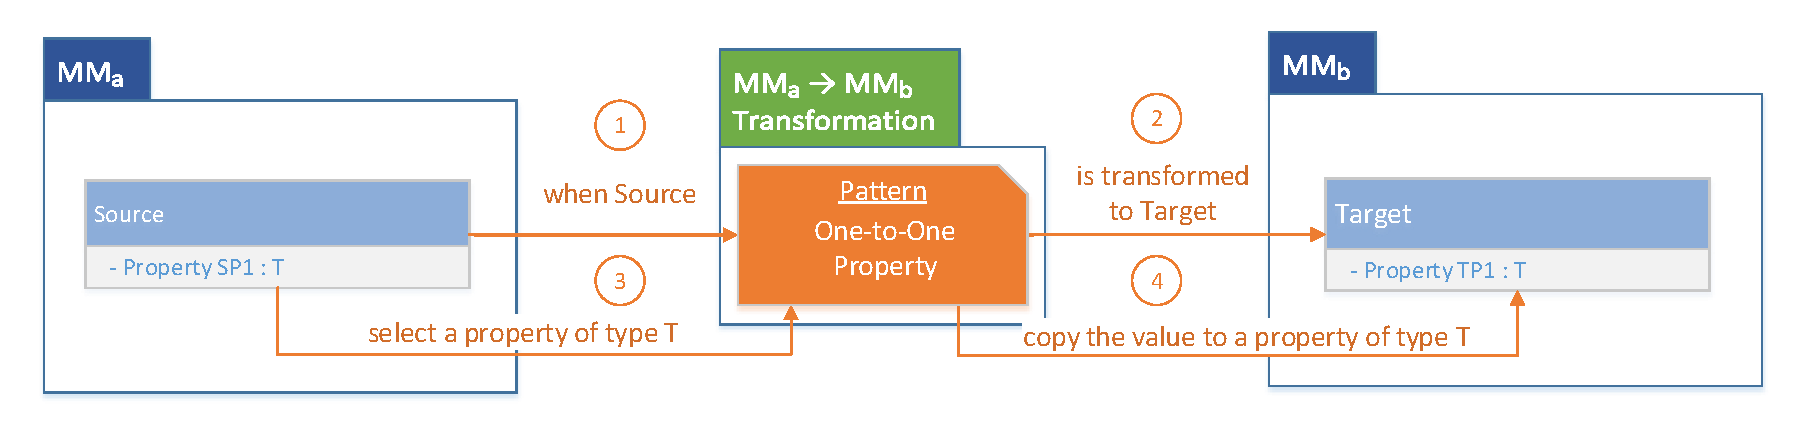
\includegraphics[scale=0.48, trim=0cm 0cm 0cm 0cm, clip=true]{Images/TransformationPattern_OneToOneProperty.pdf} 
	\caption{Transformation Pattern: One-to-One Property}
	\label{figTransformationPattern_OneToOneProperty}
\end{figure} 
 
\textbf{One-to-One Property}: Equivalent to the ``One-to-One Object" pattern on \gls{Class} level, this pattern follows the same concept on the \gls{Property} level. This pattern describes the transformation of a \gls{Property} of type Source from MM$_a$ into a \gls{Property} of the same type in Target from MM$_b$ which is required in both scenarios (see figure \ref{figTransformationPattern_OneToOneProperty}).

%  - Add + Replace:
%	- AddPropertyMapping
%	(- AddPropertyPairMapping
%	- AddRuleWithNameMapping)
%  - Remove: RemoveRule 
% => improve ``maintainability": avoid setting the same property multiple times (with different values...)
  
\begin{figure}[!ht]
	\centering
	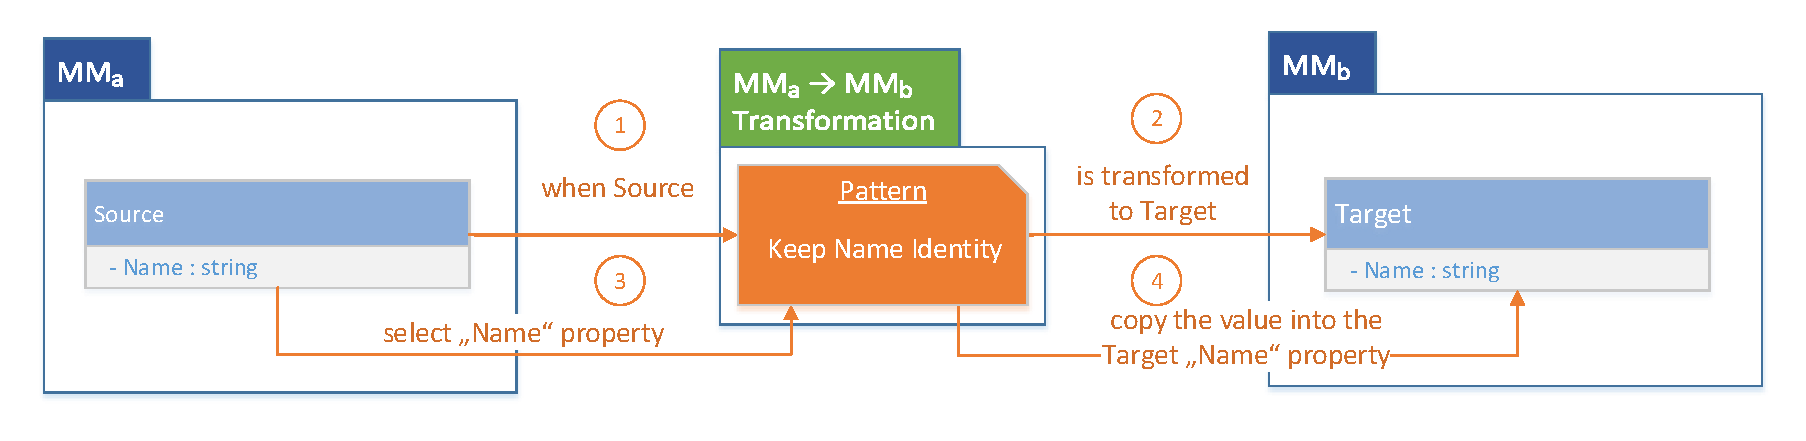
\includegraphics[scale=0.48, trim=0cm 0cm 0cm 0cm, clip=true]{Images/TransformationPattern_KeepNameIdentity.pdf} 
	\caption{Transformation Pattern: Keep Name Identity}
	\label{figTransformationPattern_KeepNameIdentity}
\end{figure} 
 
\textbf{Keep Name Identity}: Since some \glspl{FitnessFunction} require the ``Name" \gls{Property} as the identity of an \gls{Object}, this has to be kept in simple transformations. This pattern describes the conservation of the ``Name" which is required in both scenarios (see figure \ref{figTransformationPattern_KeepNameIdentity}). However, this pattern has no individual add-\gls{Mutation}, because there are two other pattern which contain this one. First, ``One-to-One Object" pattern ensures that the ``Name" is kept. Second, the ``One-to-One Property" pattern is a super set of this pattern.

%  - Add + Replace:
%	- AddRuleWithNameMapping
%	- AddPropertyMapping
%  - Remove:
%	- RemoveRule
	
\begin{figure}[!ht]
	\centering
	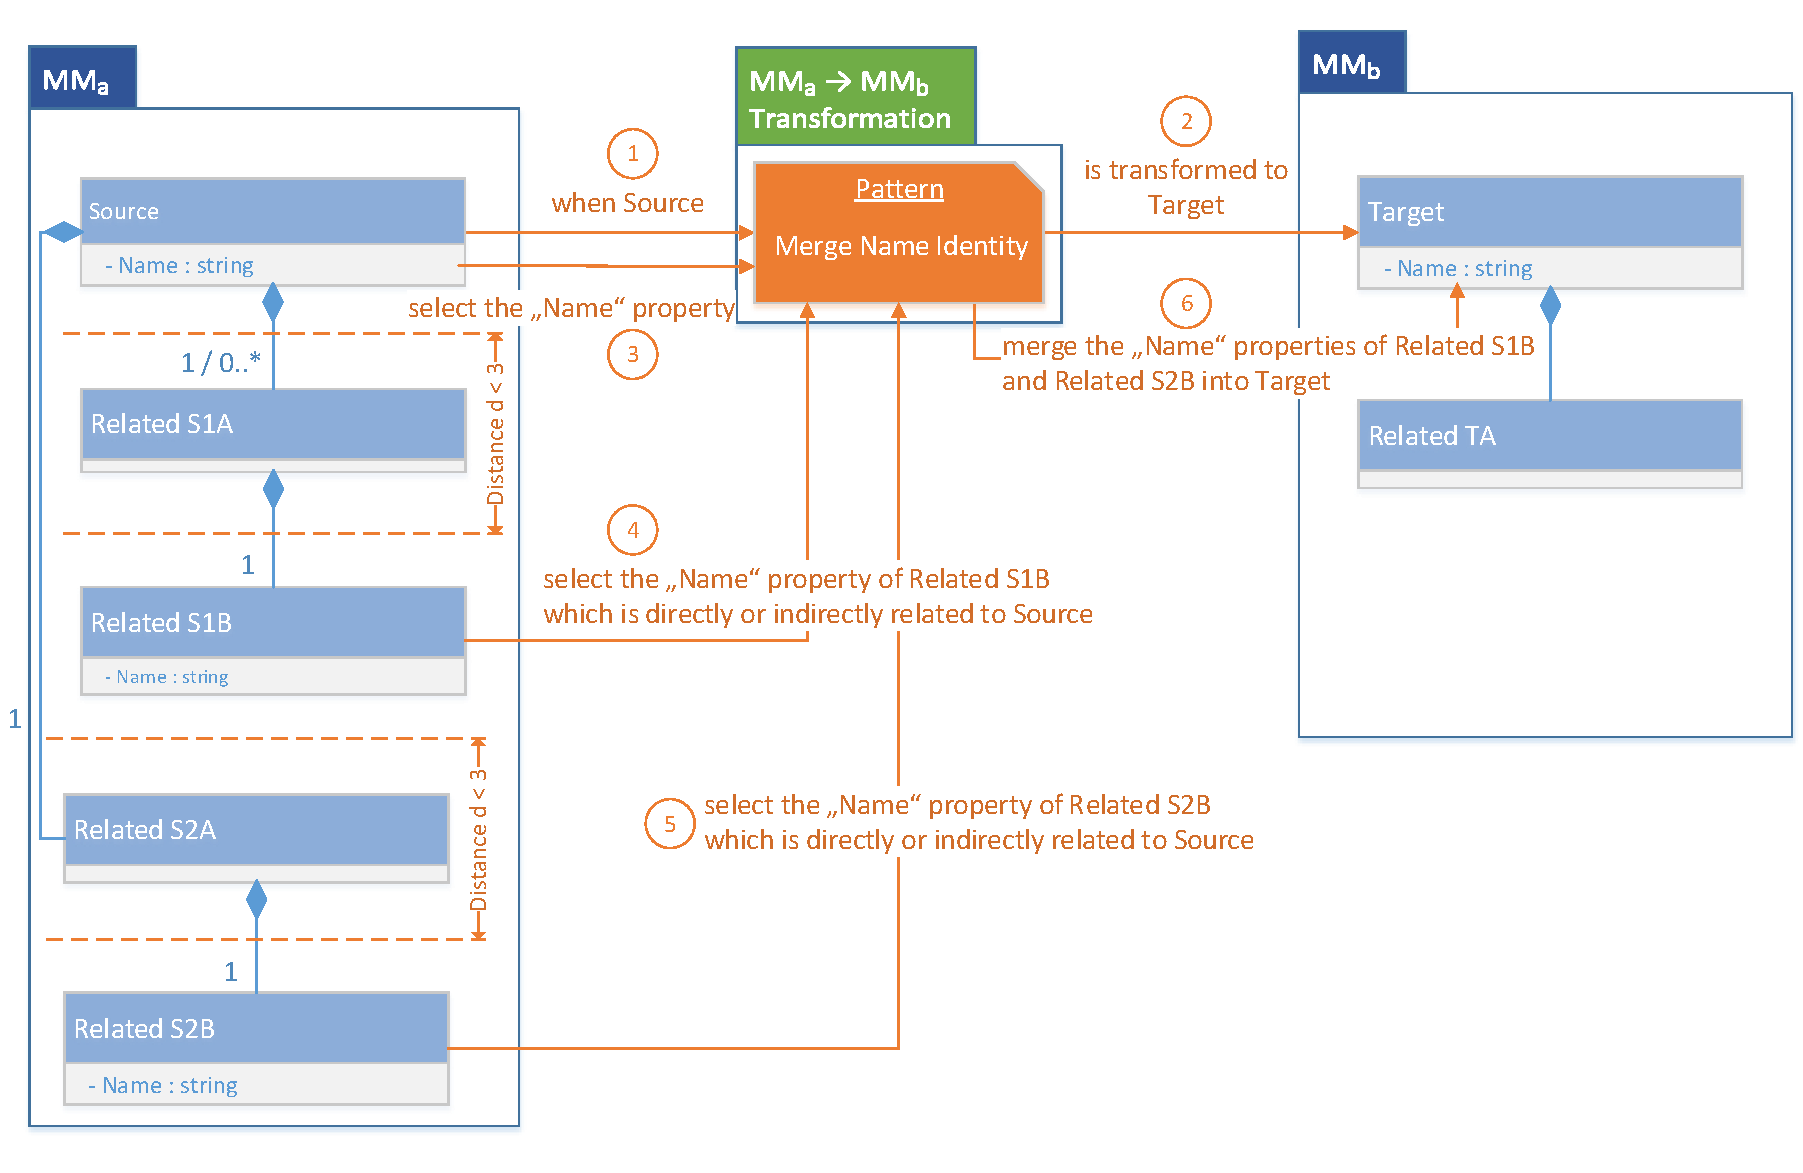
\includegraphics[scale=0.48, trim=0cm 0cm 0cm 0cm, clip=true]{Images/TransformationPattern_MergeNameIdentity.pdf} 
	\caption{Transformation Pattern: Merge Name Identity}
	\label{figTransformationPattern_MergeNameIdentity}
\end{figure} 
 
\textbf{Merge Name Identity}: Besides having to keep the ``Name" \gls{Property}, there are situations in the complex scenario where it is not that simple. Transitions describe the connection of two States and hence their ``Name" is based on this relationship like ``State1 $\rightarrow$ State2". In the case this relationship changes, the name has to be changed, too. The more general concept is to define the ``Name" based on associated \glspl{Object} which results into this pattern (see figure \ref{figTransformationPattern_MergeNameIdentity}). Similar to the ``One Object-to-Many Objects of same Type" pattern, the context is analyzed in a distance less than three and pairs of \glspl{Object} are created as \gls{Mutation} options. The ``Name" of each pair is used to assemble a new ``Name" in the form ``Name1 $\rightarrow$ Name2". Referring to section \ref{secTransformationComplexity}, this is a calculated \gls{Property}.

%  - Add + Replace:
%	- AddPropertyPairMapping
%  - Remove:
%	- RemoveRule

\subsection{Association Transformation} 	
  
\begin{figure}[!ht]
	\centering
	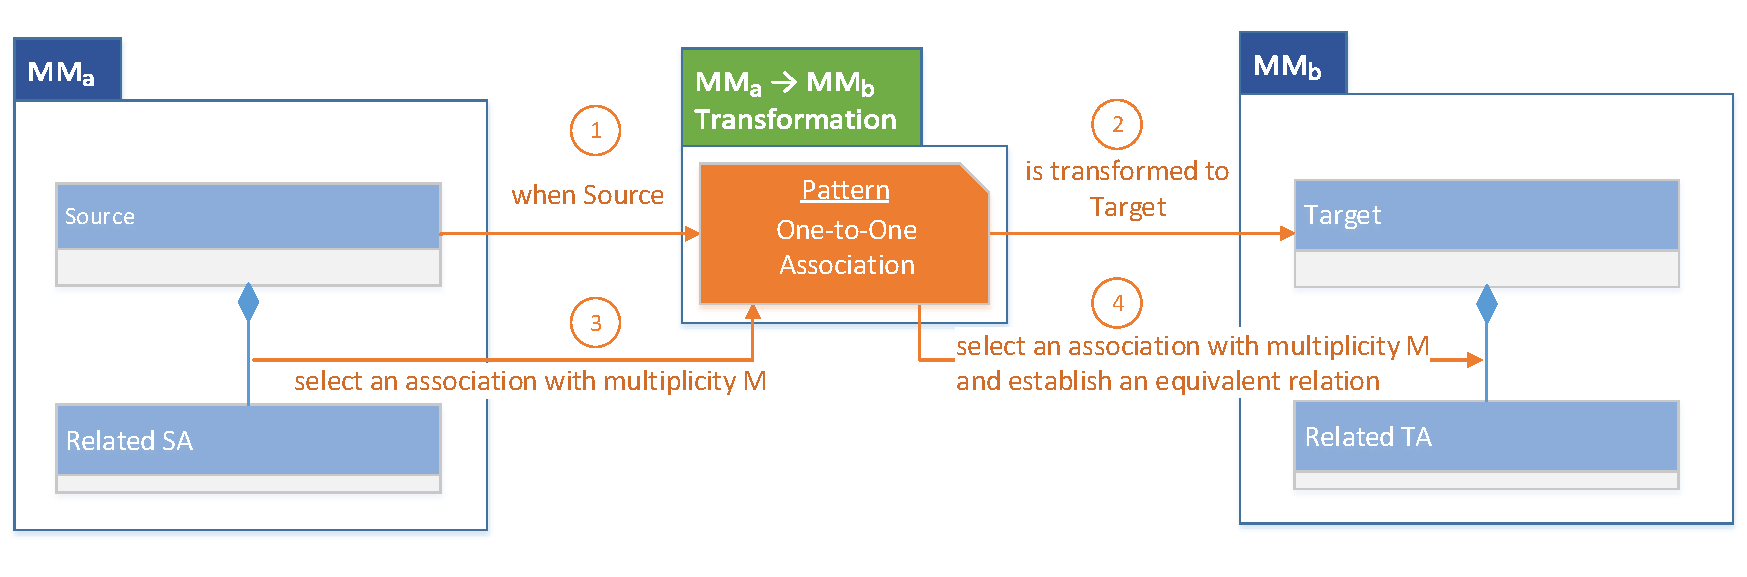
\includegraphics[scale=0.48, trim=0cm 0cm 0cm 0cm, clip=true]{Images/TransformationPattern_OneToOneAssociation.pdf} 
	\caption{Transformation Pattern: One-to-One Association}
	\label{figTransformationPattern_OneToOneAssociation}
\end{figure}

\textbf{One-to-One Association}: As already observed on the \gls{Class} and \gls{Property} level, the first pattern is the transformation of a single \gls{Association} of the Source type from MM$_a$. It is transformed into a single \gls{Association} with the same multiplicity of the Target type from MM$_b$ (see figure \ref{figTransformationPattern_OneToOneAssociation}). Both scenarios require this pattern, but it does not have an individual add-\gls{Mutation} since \glspl{Association} relate \glspl{Property} according to the simplified \gls{MetaObjectFacility} (see sub-section \ref{secModelLanguage}). Hence, the add-\gls{Mutation} of the ``One-to-One Property" pattern is used.

%  - Add + Replace:
%	- AddPropertyMapping
%  - Remove: RemoveRule
  
\begin{figure}[!ht]
	\centering
	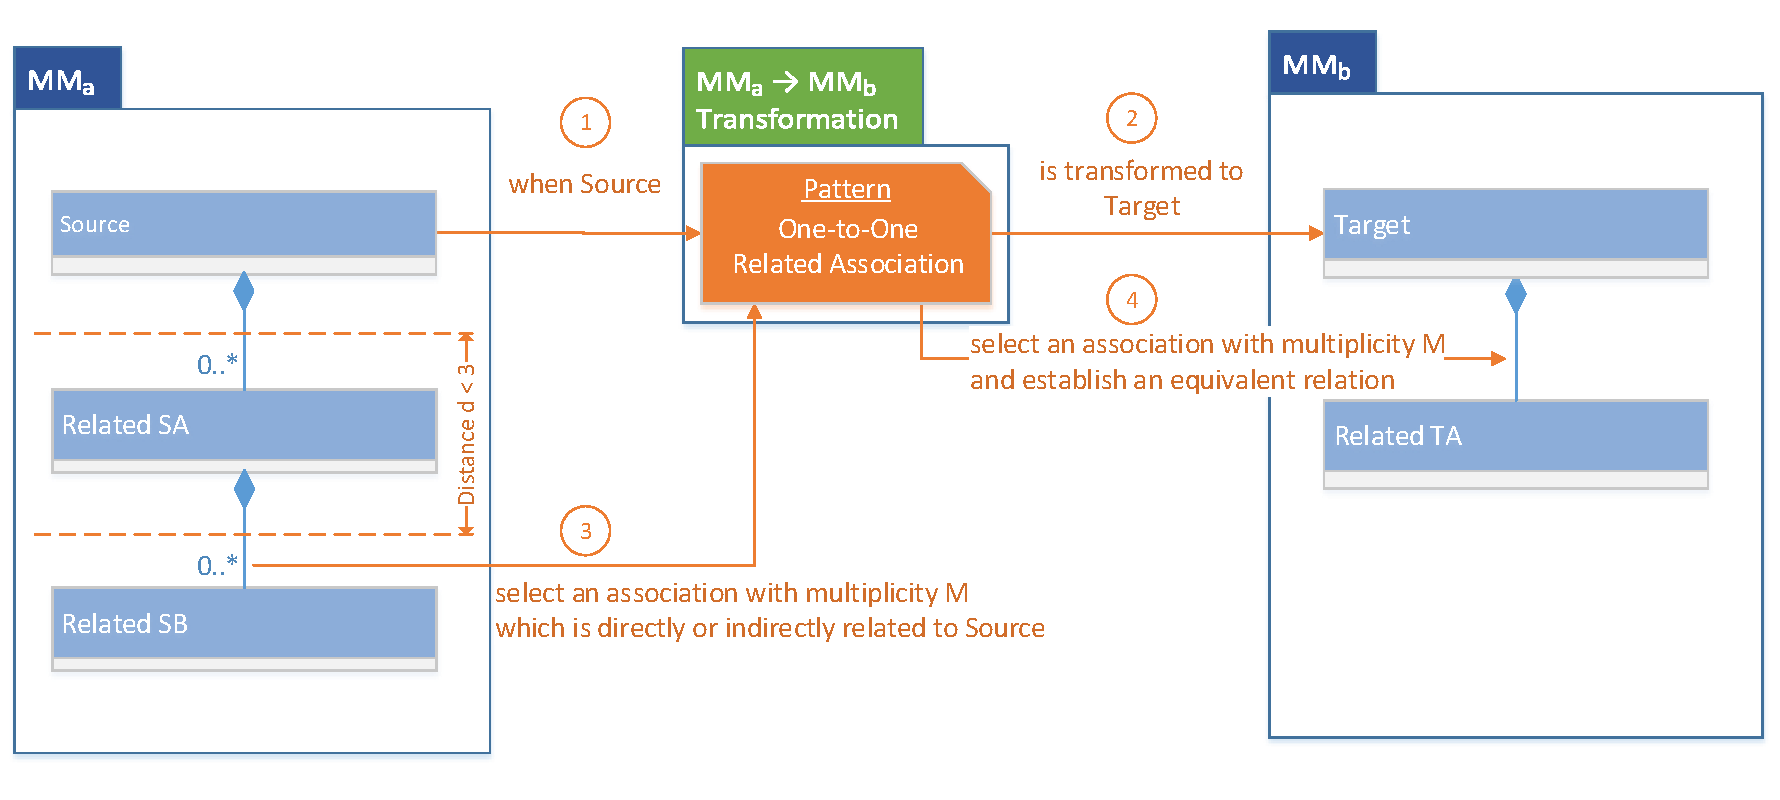
\includegraphics[scale=0.48, trim=0cm 0cm 0cm 0cm, clip=true]{Images/TransformationPattern_OneToOneRelatedAssociation.pdf} 
	\caption{Transformation Pattern: One-to-One Related Association}
	\label{figTransformationPattern_OneToOneRelatedAssociation}
\end{figure}

\textbf{One-to-One Related Association}: In the complex scenario the Transitions pointing to a complex state have to be replaced by Transitions pointing to the Initial State of the Complex State (see section \ref{secM2MScenarioBehavioralComplex}). The derived pattern is to transform an indirectly related \gls{Association} of the Source type from MM$_a$ into a directly related \gls{Association} of the Target type from MM$_b$ (see figure \ref{figTransformationPattern_OneToOneAssociation}). The distance is limited to less than three in order to avoid the excessive creation of \gls{Mutation} options as already in similar previous pattern. 

%  - Add + Replace:
%	- AddPropertyMapping
%  - Remove: RemoveRule 
   
%  => justify requirement by referring to scenarios - matrix? meta model??

%Mutations:
%- AddPropertyMapping
%- AddPropertyPairMapping
%- AddRuleOneToManyOfSameKind
%- AddRuleWithNameMapping
%- RemoveRule
%- SplitRuleAndAddGuardsForSuperclasses

\section{Fitness Functions}
\label{secFitnessFunctions}

The \gls{FitnessFunction} execution has two phases shown in listing \ref{lstFitnessEvaluatorOverview}. At first, the comparison of the \glspl{Model} M$_b$ and M$_b^*$ using the ``Comparator" results in a list of differences. Those are aggregated within a ``Comparison" to the number of matched \glspl{Class}, \glspl{Property} and \glspl{Association}. Thereafter, the rating of those results in a fitness value between 0\% and 100\% (see section \ref{secAlgorithmOverview}). The fitness value is thereby calculated using a weighted function. Since there are several options for the ``Comparator" and the ``Weights", multiple \glspl{FitnessFunction} have been designed and evaluated (see chapter \ref{chapEvaluation}) in order to identify the differences.

\begin{lstlisting}[language=PSEUDO,caption={Overview of fitness evaluation in pseudo code},label={lstFitnessEvaluatorOverview},mathescape]
module FitnessEvaluator {
	evaluate($M_b$, $M_b^*$, Comparator comparator, Weights weights) {
	
		// Phase 1: Object graph comparison
		Comparison comparison = comparator.compare($M_b$, $M_b^*$)
		
		// Phase 2: use the defined fitness function to compute the fitness
		return fitness(weights, comparison)	
	}
}
\end{lstlisting}

In the following the used comparison methods are presented in sub-section \ref{secObjectGraphComparisonMethods}, the generic \gls{FitnessFunction} in sub-section \ref{secGenericFitnessFunction} and the used configurations in sub-section \ref{secFitnessFunctionConfigurations}.

%$$compare(m, v; M_b, M_b^*)$$

%\begin{align*}
%  \text{where}~m &= \{nameidentity,heuristic,nameidentitywithheuristicfallback\} \\
%  v &= \{{c_f},{c_e},{p_f},{a_f}\}\\
%\end{align*}


%$$fitness(M_b, M_b^*, m, c_w, c_{we}, p_w, a_w) = $$
%$$fitness(c_w,compare(m,c_f;M_b, M_b^*),compare(m,c_e;M_b, M_b^*),p_w,compare(m,p_f;M_b, M_b^*),a_w,compare(m,a_f;M_b, M_b^*))$$


\subsection{Object Graph Comparison Methods}
\label{secObjectGraphComparisonMethods}

Comparing the \gls{Object} graphs of M$_b$ and M$_b^*$ is realized in three ways. The first ``Name identity" comparison is based on the assumption that every \gls{Object} is identified by a unique ``Name" \gls{Property}. This is assumption does not hold for any scenario, but for the presented ones. The second comparison approach is based on a heuristic matching. It compares \glspl{Object} based on their \glspl{Association} and \glspl{Property} and is defined within EMF Compare (see \cite{EclipseFoundation2014b}). In the following it is referred to as ``Heuristic". Finally, the third comparison method ``Name identity with heuristic fall-back" is a combination of the two. It matches \glspl{Object} based on the ,,Name" and if there is no result, uses the heuristic as a fall-back. The heuristic is derived from \cite{EclipseFoundation2014c} and presented in the following.

The $distance(a,b)$ between two \glspl{Object} a and b is the sum of all \gls{Property} changes $c(p)$. Whereas primitive \gls{Property} changes, which are only "Name" \gls{Property} changes in both scenarios, have a higher weight $w(p)$ than \gls{Association} changes. These values have been determined empirically by \cite{EclipseFoundation2014c}. Changes of string \glspl{Property} are measured by the Dice Coefficient \cite{Jaccard1912} similarity function. It results in more granular increments for those. In both scenarios this is applied to the "Name" \gls{Property}. Whereas only in the complex scenario is an increment when creating the new Transitions with the "Merge Name Identity" pattern. The comparison of associated \glspl{Object} is performed by the $simplematch(a,b)$ function, which compares the type and the index. The latter is a heuristic based on the assumption that the order of the \glspl{Object} in M$_b$ and M$_b^*$ are identical.

% recursion, top down / level by level anaylsis...

$$distance(a,b) = \sum_{p \in P_{a,b}} w(p) c(p,a,b) $$

\begin{align*}
  \text{where}~
	w(p) &= \left\{
				\begin{array}{l l}
					5 & \quad \text{if $p$ is primitive}\\
					2 & \quad \text{if $p$ is member of an association}
				\end{array}\right.\\		   
	c(p) &= \left\{
				\begin{array}{l l}	
					1 - dice(a(p),b(p)) & \quad \text{if $p$ is string}\\				
					1 & \quad \text{if p is primitive and $a(p) \neq b(p)$}\\
					1 & \quad \text{if not $simplematch(a(p),b(p))$ }\\			
					0 & \quad \text{else}
				\end{array}\right.\\
	simplematch(a,b) &= (typeof(a) = typeof(b)) \land (indexof(a) = indexof(b))
\end{align*}

In order to determine, if two \glspl{Object} are equal at all, the maximum distance function $maxdistance(a,b)$ is used to filter out pairs with too many differences. The maximum is computed as the sum of all weighted \glspl{Property}, which is the largest distance. This is reduced by an empirically determined factor (see \cite{EclipseFoundation2014c}) depending on the number of \glspl{Property} $i$ in $threshold(i)$:

$$maxdistance(a,b) = threshold(|\{p \in P_{a,b}\}|) \sum_{p \in P_{a,b}} w(p)$$

\begin{align*}
  \text{where}~
	threshold(i) &= \left\{
				\begin{array}{l l}
					0 & \quad \text{if $i < 1$}\\
					0.6 & \quad \text{if $i < 3$}\\
					0.55 & \quad \text{if $i < 4$}\\
					0.465 & \quad \text{else}
				\end{array}\right.
\end{align*}

The equivalent \gls{Object} b for a given \gls{Object} a is one of the \glspl{Object} with the minimum distance. A distance is infinite in the case it is larger than the maximum distance:

$$match(a, {b_1,..,b_n}) = \min_{b \in {b_1,..,b_n}} matchdistance(a,b) $$

\begin{align*}
  \text{where}~
	matchdistance(a,b) &= \left\{
				\begin{array}{l l}
					distance(a,b) & \quad \text{if $distance(a,b) <$ } \\ 
					& \quad \text{$maxdistance(a,b)$}\\
					infinite & \quad \text{else}
				\end{array}\right.
\end{align*}


%- attrribute only "Name"
%- references equivalent by order in output
%- root must have the correct name and contain the rest.. (EMF)

%weight per change:
%	referenceChange = 2
%	attributeChange = 5
%	* 1 / "name" = 4 / "id" = 4 / reference = 2
%
%	if move: * orderChange = 1
%	if change of string -> string: * 1 - dice coefficient
%	
%	====
%	
%	if already changed --> 1 (!!))
	
	
%distance = sum all weights

%maxDistance = sum of weights of attributes with values * 0.465d

%if < maxDistance => identical

%Therefore the EMF Compare Edition Distance Function 


%EmfCompare
%\cite{EclipseFoundation2014b}
%\cite{Toulme2006}

%ProximityEObjectMatcher

%EditionDistance - ReflectiveWeightProvider (assoc diff larger distance than props), DefaultDiffEngine

%--> the distance between them computed using the number of changes required to change a to b.

%- eContainingFeature different?
%	- must not be greater than the max distance (max Distance (empirical): based on number of features, with some empirically gathered weights)
%	-> then detailed measurement:
%		- order of features is measured
%		- equality of strings measured with dice coefficient of two string's bigrams
%		- creates longest common susequence of matching props, assoc
%		- "id" and "name" have a bigger effect than other properties


\subsection{Generic Fitness Function}
\label{secGenericFitnessFunction}

The differences between M$_b$ and M$_b^*$ determined by the methods described in the previous sub-section are the foundation for the actual \gls{FitnessFunction}. This sub-section presents a generic function with several weights rendering it configurable. Those are explained in the following sub-section \ref{secFitnessFunctionConfigurations}.

According to the simplified \gls{MetaObjectFacility} (see sub-section \ref{secModelLanguage}), the instantiated \gls{MetaObjectFacility} \glspl{Class} of M$_b$ and M$_b^*$ are \glspl{Class}, \glspl{Property} and \glspl{Association}. Hence, those define the structure of the fitness function, which compares the matched elements with the expected ones in those categories. As explained, weights must be defined for each of the three \gls{MetaObjectFacility} \glspl{Class}:

$$fitness(c_w,c_f,c_e,p_w,p_f,a_w,a_f) = \frac{c_w c_f - c_{we} c_e + p_w p_f + a_w a_f}{c_w + p_w + a_w}$$

\begin{align*}
  \text{where}~c_w &= \text{weight of ``\gls{Class} fitness"}, \\
  c_f &= \frac{c_{matched}}{c_{expected}}\% = \text{``\gls{Class} fitness"},\\
  c_{we} &= \text{weight of ``\gls{Class} error"}, \\
  c_e &= \frac{c_{unexpected}}{c_{created}}\% = \text{``\gls{Class} error"}, \\  
  p_w &= \text{weight of ``Primitive \gls{Property} fitness"}, \\
  p_f &= \frac{p_{matched}}{p_{expected}}\% = \text{``Primitive \gls{Property} fitness"},\\ 
  a_w &= \text{weight of ``\gls{Association} \gls{Property} fitness"}, \\
  a_f &= \frac{a_{matched}}{a_{expected}}\% = \text{``\gls{Association} \gls{Property} fitness"},\\
%  a_{we} &= \text{weight of ``\gls{Association} error"}, \\
%  a_e &= \frac{a_{unexpected}}{a_{created}}\% = \text{``\gls{Association} error"},\\
  \text{with}~& c_w \geq c_{we} %\land a_w \geq a_{we}
\end{align*}

Since \gls{Class} instances - \glspl{Object} - are not limited by the \gls{MetaModel}, there can be unexpected ones in M$_b^*$ which cannot be matched in M$_b$. Without any penalty in the function, the algorithm identifies \glspl{ModelToModelTransformation} as solution that create every combination of e.g. Transitions. Thus, those falsely transformed \glspl{Object} reduce the fitness in order to create a penalty and guide the algorithm in the desired way. \Glspl{Association} with an unlimited multiplicity cause such an issue, but since they are only measured through the \glspl{Property}, this error is not included in the function. %as well as \glspl{Association} with an unlimited multiplicity => associations are not evaluated in detail, just "is the property correct"

% - penalty for wrong rules and property mappings (or added constructs that cause no fitness change !?)

\subsection{Fitness Function Configurations}
\label{secFitnessFunctionConfigurations}

The previous subsections defined the comparison methods and the generic fitness function. In this section the used configurations are presented. Those are defined based on the pseudo code of the fitness evaluation shown in listing \ref{lstFitnessEvaluator}, which is an extension of listing \ref{lstFitnessEvaluatorOverview}. On the one hand, the ``Comparator" has the three realizations ``NameIdentity", ``Heuristic" and ``NameIdentityWithHeuristicFallback" (see subsection \ref{secObjectGraphComparisonMethods}). On the other hand, the ``fitness" function requires also the ``Weights" defined in subsection \ref{secGenericFitnessFunction}.

%structure Comparison {
%	attribute $c_{matched}$
%	attribute $c_{expected}$
%	attribute $c_{unexpected}$
%	attribute $c_{created}$
%	attribute $p_{matched}$
%	attribute $p_{expected}$
%	attribute $a_{matched}$
%	attribute $a_{expected}$	
%}
\begin{lstlisting}[language=PSEUDO,caption={Fitness evaluation in pseudo code},label={lstFitnessEvaluator},mathescape]
interface Comparator {
	compare($M_b$, $M_b^*$) returns Comparison;
}

module NameIdentity realizes Comparator {
	... // identifies equal objects based on their name
}

module Heuristic realizes Comparator {
	... // identifies equal objects based on the defined heuristic
}

module NameIdentityWithHeuristicFallback realizes Comparator {
	... // identifies equal objects based on their name.
		  // if their is no match, it uses the defined heuristic
}

structure Weights {
	attribute $c_w$
	attribute $c_{we}$
	attribute $p_w$
	attribute $a_w$
}

module FitnessEvaluator {
	evaluate($M_b$, $M_b^*$, Comparator comparator, Weights weights) {
	
		// Phase 1: Object graph comparison
		Comparison comparison = comparator.compare($M_b$, $M_b^*$)
		
		// Phase 2: use the defined fitness function to compute the fitness
		return fitness(weights, comparison)	
	}
}
\end{lstlisting}

The following \gls{FitnessFunction} configurations are defined based on the comparison methods and function weights. Since there are infinite weights assignable, it is not possible to create all configurations. Hence, a few are selected in this sub-section and evaluated in chapter \ref{chapEvaluation}.

%BalancedFitnessFunction
\textbf{Class focused using Name}: A correct \gls{Class} transformation is a prerequisite for the analysis of further transformations. This is especially crucial, when using the ``Name identity" comparison method. This configuration focuses the algorithm on the identification of \gls{Class} at first. It is expected that having a correct \gls{Class} transformation at first is useful, since any change of such a transformation has an impact on the contained \glspl{Property} and related \glspl{Association}. Thus, changing an existing \gls{Class} transformation reverts all related changes as well.

$$evaluate(M_b, M_b^*, Comparator, Weights)$$
\begin{align*}
  \text{where}~Comparator &= \text{NameIdentity}, \\
  Weights.c_w &= \text{2}, \\
  Weights.c_{we} &= \text{1}, \\
  Weights.p_w &= \text{1}, \\
  Weights.a_w &= \text{1} \\
\end{align*}

%StructureFocusedFitnessFunction
\textbf{More class focused using Name}: In order to evaluate the relevance of assigning \glspl{Class} more weight, this configuration increases the difference compared to the first one.

$$evaluate(M_b, M_b^*, Comparator, Weights)$$
\begin{align*}
  \text{where}~Comparator &= \text{NameIdentity}, \\
  Weights.c_w &= \text{10}, \\
  Weights.c_{we} &= \text{1}, \\
  Weights.p_w &= \text{1}, \\
  Weights.a_w &= \text{1} \\
\end{align*}

%BalancedFitnessFunctionBasedOnlyOnStructure
\textbf{Class focused using heuristic}: Evaluating the difference between the ,,Heuristic" comparison method and the two others requires this configuration.

$$evaluate(M_b, M_b^*, Comparator, Weights)$$
\begin{align*}
  \text{where}~Comparator &= \text{Heuristic}, \\
  Weights.c_w &= \text{2}, \\
  Weights.c_{we} &= \text{1}, \\
  Weights.p_w &= \text{1}, \\
  Weights.a_w &= \text{1} \\
\end{align*}

%BalancedFitnessFunctionBasedOnStructureAsFallback
\textbf{Class focused using Name and heuristic fall-back}: Evaluating the difference between the ,,Name identity with heuristic fall-back" comparison method and the two others requires this configuration.

$$evaluate(M_b, M_b^*, Comparator, Weights)$$
\begin{align*}
  \text{where}~Comparator &= \text{NameIdentityWithHeuristicFallback}, \\
  Weights.c_w &= \text{2}, \\
  Weights.c_{we} &= \text{1}, \\
  Weights.p_w &= \text{1}, \\
  Weights.a_w &= \text{1} \\
\end{align*}

%BalancedFitnessFunctionBasedOnStructureAsFallbackAndImportantAssociations
\textbf{Class and association focused using name and heuristic fall-back}: Since the heuristic utilized the \glspl{Association} in order to transform \glspl{Class}, this configuration increases the weight for those, too.

$$evaluate(M_b, M_b^*, Comparator, Weights)$$
\begin{align*}
  \text{where}~Comparator &= \text{NameIdentityWithHeuristicFallback}, \\
  Weights.c_w &= \text{2}, \\
  Weights.c_{we} &= \text{1}, \\
  Weights.p_w &= \text{1}, \\
  Weights.a_w &= \text{2} \\
\end{align*}

%PropertyFocusedFitnessFunctionBasedOnStructureAsFallback
\textbf{Property focused using Name and heuristic fall-back}: In order to provide a counter-example for the \gls{Class} emphasis, this configuration is defined.

$$evaluate(M_b, M_b^*, Comparator, Weights)$$
\begin{align*}
  \text{where}~Comparator &= \text{NameIdentityWithHeuristicFallback}, \\
  Weights.c_w &= \text{1}, \\
  Weights.c_{we} &= \text{1}, \\
  Weights.p_w &= \text{3}, \\
  Weights.a_w &= \text{3} \\
\end{align*}

%- BalancedFitnessFunction
%		double mofClassFitness = (maximumFitness / numberOfMofClassInstancesInManuallyCreatedModel) * (numberOfMofClassInstancesInManuallyCreatedModel - numberOfnotMappedMofClassInstances);
%		double mofClassError = numberOfMofClassInstancesInOutputModelOfIndividual > 0 ? (numberOfunexpectedMappedMofClassInstances / numberOfMofClassInstancesInOutputModelOfIndividual) * maximumFitness : 0;
%		double mofPropertyFitness = (maximumFitness / numberOfMofPropertiesInManuallyCreatedModel) * (numberOfMofPropertiesInManuallyCreatedModel - (numberOfNotMappedMofPropertiesInNotMappedClasses + numberOfnotMappedMofPropertiesInMappedMofClassesWithAssociations));
%
%		double fitness = (mofClassFitness * 2 - mofClassError + mofPropertyFitness) / 3.;
%		return fitness < 0. ? 0. : fitness;
%
%- BalancedFitnessFunctionBasedOnlyOnStructure
%- BalancedFitnessFunctionBasedOnStructureAsFallback
%
%- BalancedFitnessFunctionBasedOnStructureAsFallbackAndImportantAssociations
%		double mofClassFitness = (maximumFitness / numberOfMofClassInstancesInManuallyCreatedModel) * (numberOfMofClassInstancesInManuallyCreatedModel - numberOfnotMappedMofClassInstances);
%		double mofClassError = numberOfMofClassInstancesInOutputModelOfIndividual > 0 ? (numberOfunexpectedMappedMofClassInstances / numberOfMofClassInstancesInOutputModelOfIndividual) * maximumFitness : 0;
%
%		int numberOfMofPropertiesInManuallyCreatedModelExcludingAssocations = numberOfMofPropertiesInManuallyCreatedModel - numberOfMofAssociationPropertiesInManuallyCreatedModel;
%		int numberOfNotMappedMofPropertiesInNotMappedClassesExcludingAssociations = numberOfNotMappedMofPropertiesInNotMappedClasses - numberOfNotMappedMofAssociationPropertiesInNotMappedClasses;
%		int numberOfnotMappedMofPropertiesInMappedMofClassesExcludingAssociations = numberOfnotMappedMofPropertiesInMappedMofClassesWithAssociations - numberOfnotMappedMofAssociationPropertiesInMappedMofClasses;
%		double mofPropertyFitness = (maximumFitness / numberOfMofPropertiesInManuallyCreatedModelExcludingAssocations)
%				* (numberOfMofPropertiesInManuallyCreatedModelExcludingAssocations - (numberOfNotMappedMofPropertiesInNotMappedClassesExcludingAssociations + numberOfnotMappedMofPropertiesInMappedMofClassesExcludingAssociations));
%		double mofAssociationPropertyFitness = (maximumFitness / numberOfMofAssociationPropertiesInManuallyCreatedModel)
%				* (numberOfMofAssociationPropertiesInManuallyCreatedModel - (numberOfNotMappedMofAssociationPropertiesInNotMappedClasses + numberOfnotMappedMofAssociationPropertiesInMappedMofClasses));
%
%		double fitness = (mofClassFitness * 2 - mofClassError + mofAssociationPropertyFitness * 2 + mofPropertyFitness) / 5.;
%		return fitness < 0. ? 0. : fitness;
%
%- PropertyFocusedFitnessFunctionBasedOnStructureAsFallback
%		double mofClassFitness = (maximumFitness / numberOfMofClassInstancesInManuallyCreatedModel) * (numberOfMofClassInstancesInManuallyCreatedModel - numberOfnotMappedMofClassInstances);
%		double mofClassError = numberOfMofClassInstancesInOutputModelOfIndividual > 0 ? (numberOfunexpectedMappedMofClassInstances / numberOfMofClassInstancesInOutputModelOfIndividual) * maximumFitness : 0;
%		double mofPropertyFitness = (maximumFitness / numberOfMofPropertiesInManuallyCreatedModel) * (numberOfMofPropertiesInManuallyCreatedModel - (numberOfNotMappedMofPropertiesInNotMappedClasses + numberOfnotMappedMofPropertiesInMappedMofClassesWithAssociations));
%
%		double fitness = (mofClassFitness - mofClassError + mofPropertyFitness * 3) / 4.;
%		return fitness < 0. ? 0. : fitness;
%- StructureFocusedFitnessFunction
%		double mofClassFitness = (maximumFitness / numberOfMofClassInstancesInManuallyCreatedModel) * (numberOfMofClassInstancesInManuallyCreatedModel - numberOfnotMappedMofClassInstances);
%		double mofClassError = numberOfMofClassInstancesInOutputModelOfIndividual > 0 ? (numberOfunexpectedMappedMofClassInstances / numberOfMofClassInstancesInOutputModelOfIndividual) * maximumFitness : 0;
%		double mofPropertyFitness = (maximumFitness / numberOfMofPropertiesInManuallyCreatedModel) * (numberOfMofPropertiesInManuallyCreatedModel - (numberOfNotMappedMofPropertiesInNotMappedClasses + numberOfnotMappedMofPropertiesInMappedMofClassesWithAssociations));
%
%		double fitness = ((mofClassFitness - mofClassError) * 10 + mofPropertyFitness) / 11.;
%		return fitness < 0. ? 0. : fitness;
%
\newpage
\section{Selection and Replacement Strategies}
\label{secSelectionReplacementStrategies}

The \gls{SelectionStrategy} and \gls{ReplacementStrategy} control the evolution of the \gls{Population} (see sub-section \ref{secEvolutionaryAlgorithms}). There are many different strategies which can be adapted and combined. Hence, only a sub-set can be used which is presented in this section.

\begin{figure}[!ht]
	\centering
	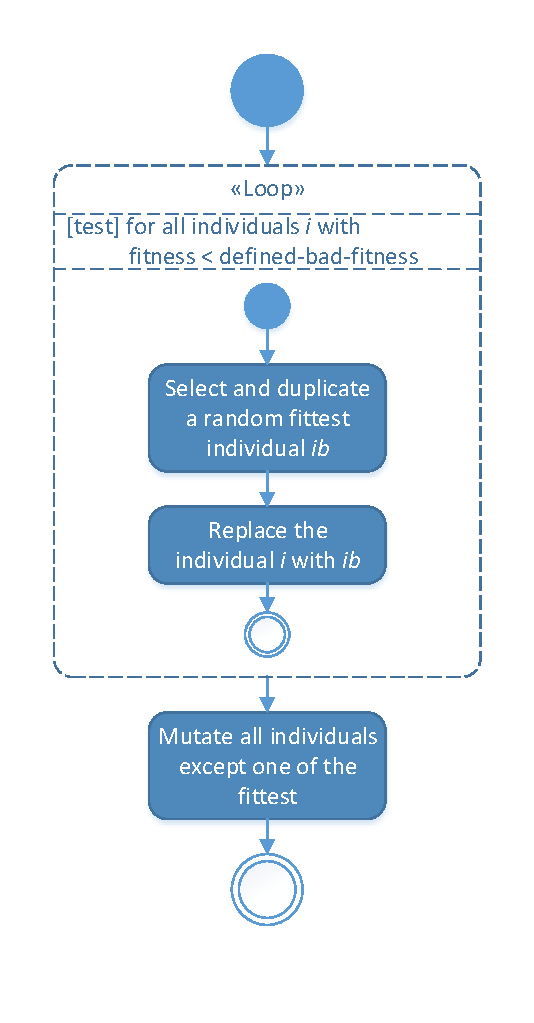
\includegraphics[scale=0.7, trim=0cm 1.5cm 0cm 0.5cm, clip=true]{Images/SelectionAndReplacement_Naive.pdf} 
	\caption{\Gls{SelectionStrategy} and \gls{ReplacementStrategy}: Naive approach with high selection pressure and elitism}
	\label{figSelectionAndReplacement_Naive}
\end{figure}

\textbf{Naive approach with high selection pressure and elitism}: The first approach is presented in figure \ref{figSelectionAndReplacement_Naive} and follows a simple ``high selection pressure" concept. In the strategy all \glspl{Individual} with a bad-fitness, which is defined as 2\%, are replaced by randomly selected duplicates of the fittest. Afterwards, all \glspl{Individual}, except one of the best, are mutated. A best one is kept in order to ensure a monotonically increasing \gls{FitnessFunction} for the \gls{Population}. The strategy exploits and improves currently promising \glspl{CandidateSolution} fast. It also tries to advance all with a fitness between 2\% and 100\%, which are expected to be many. This benefit creates the risk of getting trapped in a \gls{LocalOptimum} and requires a lot of computational power, since almost all \glspl{Individual} are mutated always. % At least 10 \glspl{Individual} are kept in any case, even when all are below 2\% to

\begin{figure}[!ht]
	\centering
	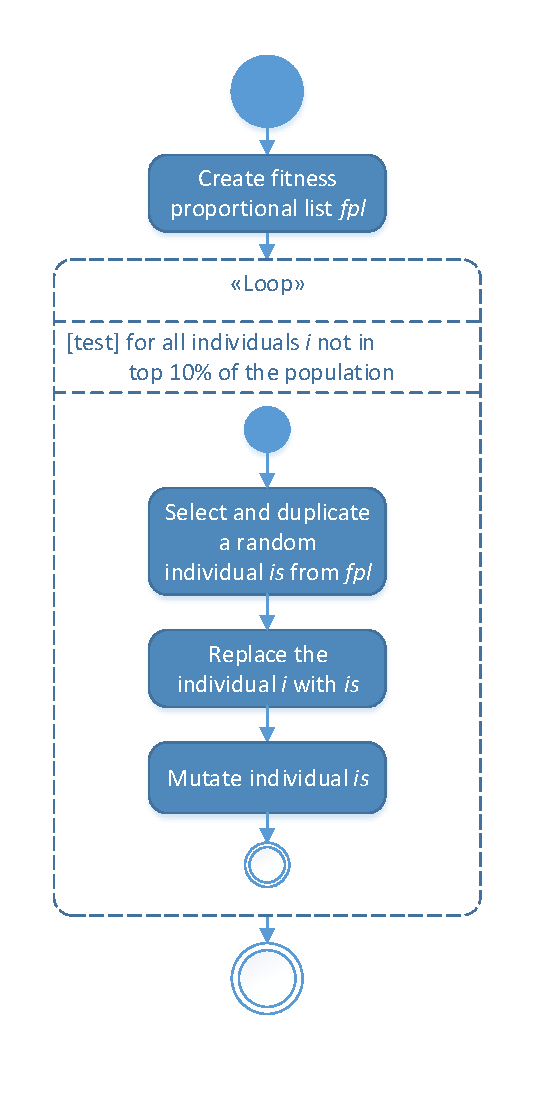
\includegraphics[scale=0.7, trim=0cm 1.5cm 0cm 0.5cm, clip=true]{Images/SelectionAndReplacement_Roulette.pdf} 
	\caption{\Gls{SelectionStrategy} and \gls{ReplacementStrategy}: \Gls{RouletteWheelSelection} with elitism}
	\label{figSelectionAndReplacement_Roulette}
\end{figure}

\textbf{\Gls{RouletteWheelSelection} with elitism}: In order to reduce the change of getting trapped in \gls{LocalOptimum}, the second strategy uses \gls{RouletteWheelSelection} (see sub-section \ref{secEvolutionaryAlgorithms}). Furthermore, instead of using a bad-fitness-constant for the replacement, a fixed fraction of the \glspl{Individual} is used. Since this strategy imposes a greater chance for \glspl{Individual} with bad fitness, it might slow down otherwise.

This strategy creates a fitness proportional list of all \glspl{Individual}. It then replaces all \glspl{Individual} which are not in the top 10\% of the \gls{Population} with duplicates of those (see figure \ref{figSelectionAndReplacement_Roulette}). After the replacement the duplicates are mutated.

\begin{figure}[!ht]
	\centering
	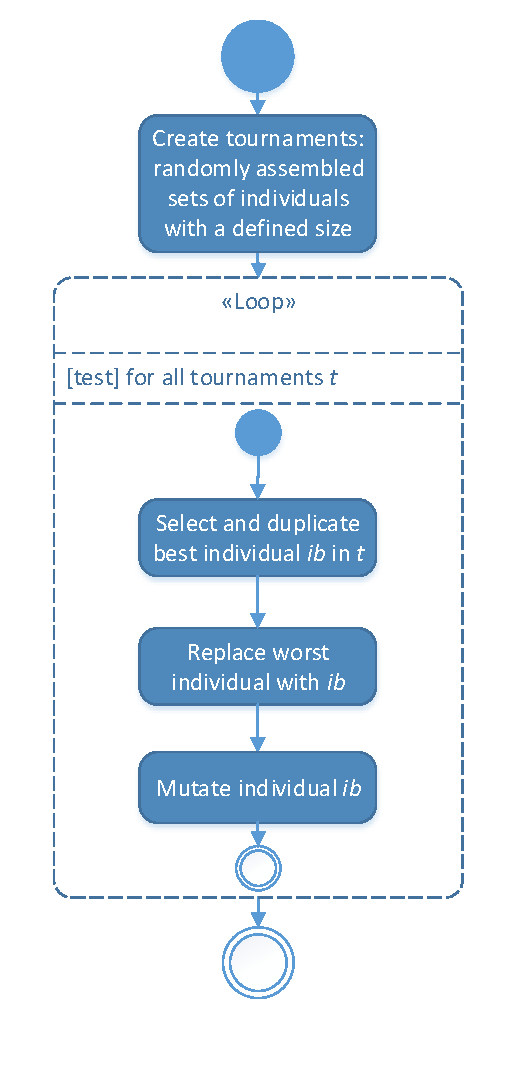
\includegraphics[scale=0.7, trim=0cm 1cm 0cm 0cm, clip=true]{Images/SelectionAndReplacement_Tournament.pdf} 
	\caption{\Gls{SelectionStrategy} and \gls{ReplacementStrategy}: \Gls{TournamentSelection} with elitism}
	\label{figSelectionAndReplacement_Tournament}
\end{figure}

\textbf{\Gls{TournamentSelection} with elitism}: This strategy uses \gls{TournamentSelection} and thus the selection pressure and the required computational power can be fine-tuned by adjusting the tournament size. At first, the tournaments are created with the defined size. A tournament is a randomly assembled proper subset, whereas the intersection of all subsets is empty. Within each the best \gls{Individual} replaces the worst, which is also mutated (see figure \ref{figSelectionAndReplacement_Tournament}). The others remain unchanged. A larger tournament size increases the selection pressure and decreases the required computational power. The strategy is used with a tournament size of two, which is the minimum, and 10.

% use the previously explained \gls{FitnessFunction} and \glspl{Mutation}
%-> ELITISM REQUIRED
%- NaiveMaximumSelectionPressureAlgorithm
%  In the first place instead of sophisticated \glspl{SelectionStrategy}, a naive approach is used which chooses simply all \glspl{Individual} for \gls{Mutation}. This should provide a large \gls{GeneticDiversity} with the risk of not always having a monotonically increasing fitness function.

	%In this phase some \glspl{Individual} are being removed from the \gls{Population}. The naive approach is to remove the ones which have a bad fitness which will be used in the first prototype. However this \gls{Selection} mechanism tends to move the whole \gls{Population} towards \gls{LocalOptimum} and might not find the \gls{GlobalOptimum}. This is because an \gls{Individual} which has a bad fitness in the first place might very well become the optimal solution later after some variations. More sophisticated selection mechanisms are for example the \gls{RouletteWheelSelection} and the \gls{TournamentSelection}. As mentioned before the usage of those advanced methods will depend on the evaluation results. 
	
	%In simple words the whole approach can be described as ``Start with nothing. Try to explore as many directions as possible from there. Follow only the ones that are promising.".
	
%The composition of the next \gls{Generation} is also based on a naive \gls{Elitism} \gls{ReplacementStrategy}. But instead of keeping a fixed number of fittest \glspl{Individual}, a threshold for ``too bad" \glspl{Individual} is being defined. All below are removed and replaced with copies of the fittest. This might limit \gls{GeneticDiversity} and end up in a \gls{LocalOptimum} in general. As the first scenario is simple and the chosen \glspl{SelectionStrategy} should produce a large \gls{GeneticDiversity} in contrast, this should in total result in a fast convergence towards the optimal solution.	

\section{Mutation Selection Strategies}
\label{secMutationSelectionStrategies}

As previously stated, the approach presented in this thesis utilizes many different \glspl{Mutation}, each defining options for a given \gls{ModelToModelTransformation}. A mutation of an \gls{Individual} is the application of a \glspl{Mutation} with a single option. Hence, the option must be selected. This can be performed in two different ways which are described in the following.

%SelectOptionFromAllPossibleDirectly
\textbf{Selection option from all possible}: The first naive strategy selects the option randomly from a list of all possible options. This provides \glspl{Mutation} with a high number of options, a higher chance to be chosen.

%SelectOperatorFirstAndThenAnOption
\textbf{Select operator first and then an option}: This strategy ensures equivalent opportunities for all \glspl{Mutation}, since those are selected randomly at first, followed by a random selection of an option.

\glsresetall
\chapter{Prototype Design}\label{chapPrototypeDesign}

% - Test driven development: per mutation operator: unit test with expected result
%	- Make fitness comparison configureable (reflect in db, graphs etc)


In the previous chapter the algorithmic approach has been presented, whereof the actual realization is described in this chapter. There are several questions that need be considered and most of them are directly related to existing software frameworks and technologies. The general requirements regarding the implementation are extensibility and the consideration of large \glspl{SearchSpace}. In the following list a short overview of the prototype design is provided:

\begin{itemize}
	\item Extensibility:
		\begin{itemize}
			\item The modular architecture and the used state-of-the-art modularization technology provide an easy integration of new components.
			\item \Glspl{Mutation} are implemented based on the \gls{AbstractSyntax} of the \gls{EpsilonTransformationLanguage}. Hence, they are not limited to the aspects of the language defined by the transformation pattern.
			\item \Glspl{Mutation} are itself implemented as \glspl{ModelToModelTransformation}. Thus, they are well-defined and can be modified and extended.
		\end{itemize}
	\item Consideration of large \glspl{SearchSpace}:
		\begin{itemize}
			\item The prototype provides a chart based evaluation with a graphical user interface. It allows the analysis of the fitness distribution and the comparison of components (i.e. the comparison of different Selection and Replacement Strategies). Thus, the effect of modifications can be analyzed especially regarding the most important issue of non-termination.
			\item Most of the components are tested by unit-tests and all by integration-tests. Especially \glspl{Mutation} are tested thoroughly. Thereby, the developer is able to identify issues resulting in non-termination.
		\end{itemize}
\end{itemize}

An overview of the architecture is presented in section \ref{secArchitectureOverview}. The following sections \ref{secThirdPartyFrameworks}, \ref{secTransformationGenerator}, \ref{secMetaModels}, \ref{secTransformationExecuter} and \ref{secFrontendAndDatabaseServer} provide details about the components.

\section{Architecture Overview}\label{secArchitectureOverview}

An overview of the components is presented in figure \ref{figPrototypeArchitectureV1Overview}. The core component is the ``Transformation Generator" that creates the desired ``MM$_a$ $\rightarrow$ MM$_b$ Transformation". It is based on the example \gls{Model} pairs M$_a$ and M$_b$, including their \glspl{MetaModel} MM$_a$ and MM$_b$. The algorithm described in chapter \ref{chapAlogrithmDesign} is realized inside this component.

The \gls{MetaModel} and \gls{Model} related operations are orchestrated through the ``\Gls{TransformationExecuter}" component. The ``Meta Models" component contains the definitions. Both are based on the underlying ``Model Transformation Language, Compiler \& Execution Engine" and ``Meta Object Facility (MOF) Framework". Those are responsible to manage the transformations in \gls{AbstractSyntax} and execute them based on their \gls{ConcreteSyntax}. Additionally, there is a ``Front-end" and a ``Database Server" component which collect and visualize detailed information about the \gls{EvolutionaryAlgorithm} behavior. 

\begin{figure}[!ht]
	\centering
	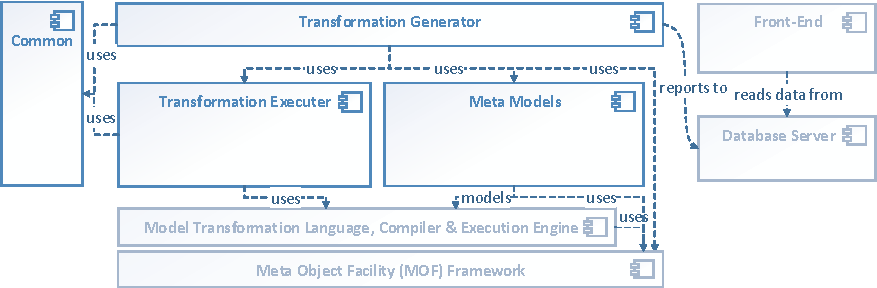
\includegraphics[scale=0.96]{Images/PrototypeArchitectureV1Overview.pdf} 
	\caption{Prototype Architecture Overview}
	\label{figPrototypeArchitectureV1Overview}
\end{figure}

The whole in-depth architecture is presented in figure \ref{figPrototypeArchitectureV1} whereas the description of the details is provided in the next sections.


\begin{landscape}
\setlength{\unitlength}{1cm}
\newsavebox{\boxPrototypeArchitectureVOne} 
\savebox{\boxPrototypeArchitectureVOne}{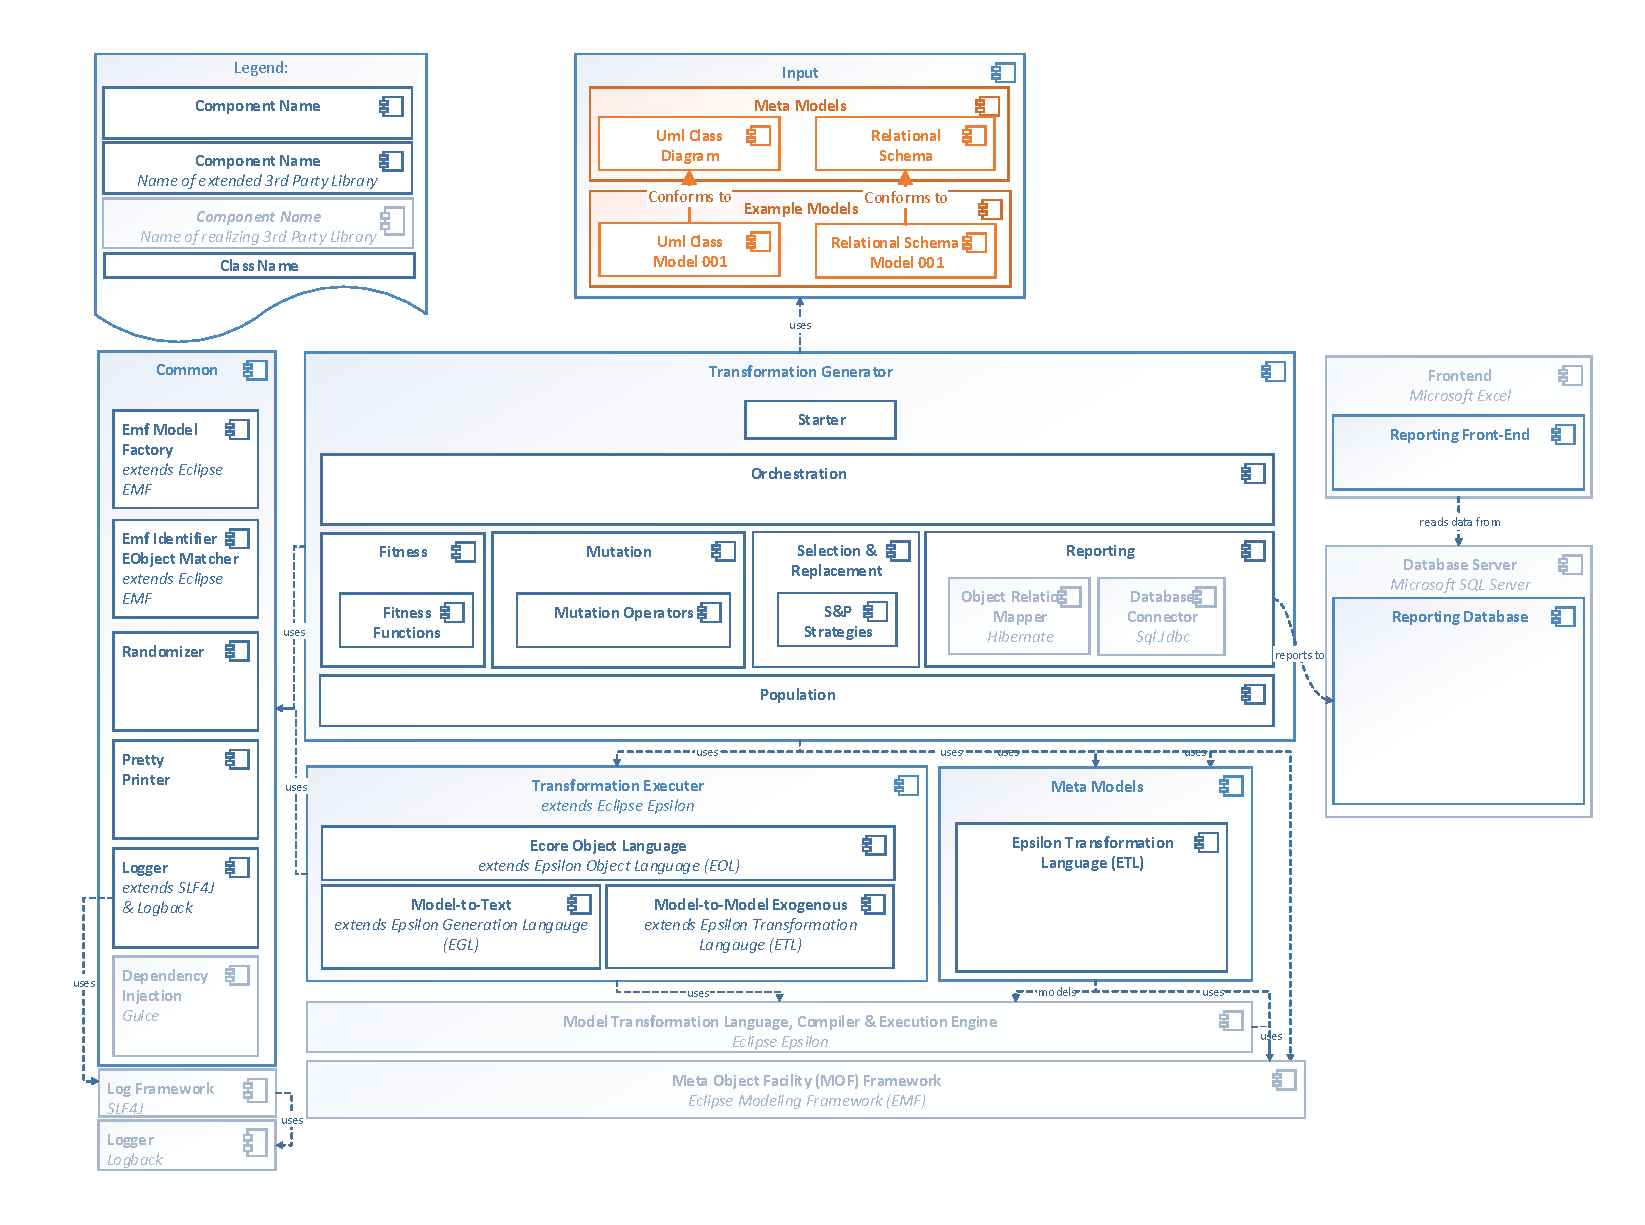
\includegraphics[scale=0.9]{Images/PrototypeArchitectureV1.pdf}} 
 \begin{figure}
   \begin{picture}(0,16.5) %-x+
  	\put(-2,0){\usebox{\boxPrototypeArchitectureVOne}} %-y+
   \end{picture} 
   \caption{Prototype Architecture}
   \label{figPrototypeArchitectureV1}  
 \end{figure}
\end{landscape}


\section{Transformation Generator}\label{secTransformationGenerator}

In order to orchestrate all the internal and external components by realizing the \gls{EvolutionaryAlgorithm}, the `Transformation Generator" is required. The main purpose is the execution of the evolution with the goal to identify a \gls{ModelToModelTransformation} for the given input \glspl{MetaModel} MM$_a$ and MM$_b$ based on the M$_a$-M$_b$ example pairs.

\subsection{Shared Data Model}
\label{secSharedDataModel}

Since the evolutionary process consists of several phases, a shared ``Population" data model is used to manage the data. This is presented in figure \ref{figPrototypeArchitectureV1PopulationDataModel}.

\begin{figure}[htb]
	\centering
	\includegraphics[scale=0.6]{Images/PrototypeArchitectureV1PopulationDataModel.pdf} 
	\caption{Prototype Population Data Model Overview}
	\label{figPrototypeArchitectureV1PopulationDataModel}
\end{figure}

%A configuration defines the settings like the \gls{FitnessFunction}, with which a \gls{Population} has been created. A \gls{Population} has the attributes ``CreatedAt" and ``CompletedAt". It consists of \glspl{Individual}, which have the attributes ``Fitness" and ``\gls{Generation}".

Based on the algorithm design in section \ref{secAlgorithmOverview}, the general structure is as follows: A \gls{Population} consists of \glspl{Individual}. Each \gls{Individual} has a ``Model" as \gls{Genotype} and a ``Program" as \gls{Phenotype}. The former contains the transformation in \gls{AbstractSyntax}, while the latter is in \gls{ConcreteSyntax}.

Since a \gls{Population} can be executed with different scenarios, \glspl{FitnessFunction}, \glspl{Mutation}, \glspl{SelectionStrategy} and \glspl{ReplacementStrategy}, all this information is stored in the ``Configuration". Additionally, there are ``ConfigurationStatistics" which contain aggregated fitness and runtime values required in the evaluation (see chapter \ref{chapEvaluation}).

With this data model the different aspects of the \gls{EvolutionaryAlgorithm} are realized in the components ``Orchestration", ``Fitness", ``Mutation" and ``Selection \& Replacement". Also, the ``Reporting" component is based on this model (see section \ref{secFrontendAndDatabaseServer}).

\subsection{Realization of Mutations}
\label{secRealizationOfMutations}

The \glspl{Mutation} are defined in section \ref{secPatternAndMutations} as a mechanism to add, remove or change a \glspl{ModelToModelTransformation} according to a pattern. In order to realize such a \gls{Mutation}, at first the \gls{Encoding} of \glspl{ModelToModelTransformation} has to be defined. There are several possibilities which are presented in the following, whereas the implemented approach is the last one:

\begin{itemize}
	\item \textbf{Simple approach based on \gls{ConcreteSyntax}}: Realize \glspl{Mutation} based on the representation of a \gls{ModelToModelTransformation} used by humans. This possibility does not provide any semantic information, which renders analysis and modifications difficult. 
	\item \textbf{Approach based on \gls{Grammar} and parse tree}: Perform a structural analysis of the transformation using its own \gls{Grammar}. Since this option still lacks precise semantic details, it is not sufficient. 
	\item \textbf{Approach based on the \gls{AbstractSyntax}}: Use the \gls{AbstractSyntax} of the \gls{TransformationExecuter}. This representation allows a precise analysis, since it is used to execute the transformation. However, it is not intended to modify the transformation. Therefore, it is designed as a super-set of the \gls{TransformationLanguage} and modifications can result in invalid transformations.
	\item \textbf{Chosen approach based on self-defined \gls{AbstractSyntax}}: In order to overcome the limitations, a new \gls{AbstractSyntax} is defined as a \gls{MetaModel}. On the one hand it enables the semantic analysis of a transformation. On the other hand it is semantically equivalent to the \gls{TransformationLanguage}. Hence, only valid modifications through \glspl{Mutation} are possible which can be designed as \glspl{ModelToModelTransformation} itself.
\end{itemize}

After providing a general overview of the realization options, the following paragraphs explain those in detail.

\textbf{Simple approach based on \gls{ConcreteSyntax}}: The first option is to implement the \glspl{Mutation} as programs that manipulate the \gls{ConcreteSyntax} of the \gls{ModelToModelTransformation}. An example for the ``One-to-One Object" add-\gls{Mutation} is a program that takes a textual representation of the transformation as an input and appends such a \gls{TransformationRule}. The drawback is that it does not scale with a large number of \glspl{Mutation}, especially in the case of sophisticated ones. Using this procedure each \gls{Mutation} needs to parse the existing transformation and add the appropriate lines of code in the right place with respect to existing constraints, which is error prone and complex.

%Therefore, the next alternatives are based on representations of the \gls{ModelToModelTransformation}, which contain semantic information. 

This representation is used to provide humans a user friendly interface, but when considering the \glspl{Mutation} there are different requirements. In general, the question is what kind of structures are allowed. For example, a \gls{TransformationRule} needs exactly one reference to a \gls{Class} of MM$_a$ and two or more to \glspl{Class} of MM$_b$. Having this knowledge, the \gls{Mutation} is able to query the kind of \glspl{Class} of MM$_a$ that are already mapped and those which are not. This is a difficult task when having only a representation like that. Without utilizing the \gls{Grammar} at all, it would result in parsing the text file. This might be a lookup for strings like ``transform", followed by an appended additional \gls{TransformationRule}. Such an append would then be a fixed string sequence, like ``rule X ...". Considering difficult expressions, which are allowed by the \gls{Grammar}, the approach is difficult to handle.

\textbf{Approach based on \gls{Grammar} and parse tree}: The next approach is to use the \gls{Grammar} to parse the existing transformation to create a parse tree representation like the one shown in figure \ref{figEtlExampleParseTree}. A simplified excerpt of this \gls{Grammar} is described in listing \ref{lstEtlGrammarFragment}, which contains two of the about 75 \glspl{ProductionRule} (see \cite{EclipseFoundation2014}) written in ANTLR 3 (\cite{Atlassian2014}). 

The first one is ``transformationRule" that defines how a \gls{TransformationRule} is structured. First, there must be the word ``rule" followed by a ``NAME" that can be any kind of string. Afterwards, there has to be a ``formalParameter" defined, which refers to a \gls{Class} of MM$_a$ and a ``formalParameterList" for one or more \glspl{Class} of MM$_b$ that are created by this \gls{TransformationRule}. Finally, a ``block" of statements has to be defined containing e.g. \gls{Property} mappings. The second \glspl{ProductionRule} is the ``formalParameter" that needs a ``NAME" and a ``typeName". The latter must refer to a \gls{Class} of MM$_a$ but that is not in scope for a \gls{Grammar}.

\begin{lstlisting}[language=ANTLR,caption={\Gls{EpsilonTransformationLanguage} specified in ANTLR \Gls{Grammar} (Simplified fragment)},label={lstEtlGrammarFragment}]
grammar EpsilonTransformationLanguage;

transformationRule
	:	'rule' NAME 
			'transform' formalParameter 
			'to' formalParameterList
			'{'
			 	block 
		'}'
	;

formalParameter
	:	NAME ':' typeName
	;
	
...
\end{lstlisting}

This allows an easier querying for existing structures, e.g. ``get all transform nodes" to analyze which \glspl{Class} of MM$_a$ have already been mapped. Since it is only used to read the transformation, not to manipulate it and write it back, this is a one-way technique. Usually, the transformation is written by humans and then parsed to be executed by the \gls{TransformationExecuter}, hence the limitation. Additionally, this representation still contains a lot of useless information in form of keywords like ``rule". This renders it difficult to mutate the parsed tree, as it on the one hand requires a lot of useless information and on the other hand is missing important information. Such an information is for example that the first ``formalParameter" must refer to a \gls{Class} of MM$_a$ or that a \gls{TransformationRule} needs exactly one ``transform" node. %The latter seems maybe not obvious as it is stated by the \gls{Grammar} but when looking at the parse tree, the information got lost as there is no direct link to the \gls{Grammar}.

\begin{figure}[htb]
	\centering
	\includegraphics[scale=0.8]{Images/EtlExampleParseTree.pdf} 
	\caption{Parse tree fragment of the simple structural example}
	\label{figEtlExampleParseTree}
\end{figure}

\textbf{Approach based on the \gls{AbstractSyntax}}: The \gls{AbstractSyntax} of the chosen \gls{TransformationLanguage} \gls{EpsilonTransformationLanguage} is not explicitly provided, but could be extracted from the \gls{TransformationGenerator} (see \cite{EclipseFoundation2014}). Since it is used to execute a transformation, this \gls{AbstractSyntax} removes all aspects and constraints which are irrelevant for this task (see \cite{Bendersky2009}). The drawback is that this is a one-way approach, where the resulting language allows constructs that were not possible before due to the simplified structure. Thereby, it becomes a super-set of the \gls{EpsilonTransformationLanguage} which renders a transformation back into the \gls{ConcreteSyntax} impossible in general. This syntax could be used, if the goal of the generated transformation would only be the execution. However, the goal is to create transformations which are maintainable by humans. Hence, the resulting transformation must be provided in \gls{ConcreteSyntax}.

\textbf{Chosen approach based on self-defined \gls{AbstractSyntax}}: Since the previous approaches were not appropriate to serve as a foundation for the \glspl{Mutation}, the solution is to define an \gls{AbstractSyntax} using a \gls{MetaModel} instead, shown in figure \ref{figEtlSimplifiedFragmentOfAbstractSyntaxWithExample}. Based on the \gls{Grammar} this \gls{MetaModel} is derived manually defining an \gls{AbstractSyntax} of the \gls{EpsilonTransformationLanguage} that on the one hand excludes all keywords, but on the other hand contains the required constraints. 

The fragment in figure \ref{figEtlSimplifiedFragmentOfAbstractSyntaxWithExample} presents the idea, which is based on the listing \ref{lstEtlGrammarFragment} and figure \ref{figEtlExampleParseTree}. The \gls{MetaModel} on the left hand side specifies the structure of a ``TransformationRule" that needs exactly one ``FormalParameter" while both need a name. Whereas the instance on the right hand side is directly based on that and is enabled for queries and modifications according to the \gls{MetaModel}. Those modifications are \glspl{ModelToModelTransformation} themselves, since they are based on \glspl{MetaModel}.

\begin{figure}[htb]
	\centering
	\includegraphics[scale=0.6]{Images/EtlSimplifiedFragmentOfAbstractSyntaxWithExample.pdf} 
	\caption{Simplified fragment of the \Gls{EpsilonTransformationLanguage} in \gls{AbstractSyntax} with an example}
	\label{figEtlSimplifiedFragmentOfAbstractSyntaxWithExample}
\end{figure}

This \gls{MetaModel} of the \gls{EpsilonTransformationLanguage} is insufficient, as it lacks the foundation of its input \glspl{MetaModel} MM$_a$ and MM$_b$, the \gls{MetaObjectFacility} \gls{MetaModel}. In order to create proper references also a simplified \gls{MetaObjectFacility} \gls{MetaModel}, based on the one from section \ref{secModelLanguage}, is added to the \gls{EpsilonTransformationLanguage} \gls{MetaModel}.

Figure \ref{figMofSimplifiedFragmentOfAbstractSyntaxWithExample} shows this extension. It contains a ``MofClass" with its ``MofProperties", both derived from a ``MofNamedElement" as each requires a ``Name". Additionally, ``MofProperties" can be associated with a ``MofAssociation" that includes at least two of them. In the context of the simple structural example, an instance of a ``MofClass" is a ``umlPackage" with a ``MofProperty" ``umlPackageName".

\begin{figure}[htb]
	\centering
	\includegraphics[scale=0.6]{Images/MofSimplifiedFragmentOfAbstractSyntaxWithExample.pdf} 
	\caption{Simplified fragment of \Gls{MetaObjectFacility} in \gls{AbstractSyntax} with an example}
	\label{figMofSimplifiedFragmentOfAbstractSyntaxWithExample}
\end{figure}

The usage of the extension is presented in figure \ref{figEtlandMofAbstractSyntaxReferenceExample}, which combines the examples from figure \ref{figEtlSimplifiedFragmentOfAbstractSyntaxWithExample} and \ref{figMofSimplifiedFragmentOfAbstractSyntaxWithExample}. As it is possible to reference to the MM$_a$ and MM$_b$ \gls{MetaModel} \glspl{Class} and \glspl{Property}, the ``umlPackage : FormalParameter" can be directly related to the ``umlPackage : MofClass".

\begin{figure}[htb]
	\centering
	\includegraphics[scale=0.6]{Images/ETLandMofAbstractSyntaxReferenceExample.pdf} 
	\caption{Example of a reference in an instance of the \gls{AbstractSyntax} of the combined \Gls{EpsilonTransformationLanguage} and \Gls{MetaObjectFacility}}
	\label{figEtlandMofAbstractSyntaxReferenceExample}
\end{figure}

Based on this \Gls{EpsilonTransformationLanguage} and \Gls{MetaObjectFacility} \glspl{MetaModel} the \glspl{Mutation} are defined. Since this is an \gls{Endogenous} transformation, there is a \gls{DomainSpecificLanguage} also in the language framework of \gls{EpsilonTransformationLanguage}, which is the \gls{EpsilonWizardLanguage} (see \cite{Kolovos2013}). This language was replaced during the implementation phase with a self-designed, embedded transformation \gls{DomainSpecificLanguage} in Java 8. Further details about this decision are provided in the sub-section \ref{ModelToModelTransformationFramework}.

Using the \gls{Mutation} specific \gls{AbstractSyntax} instead of the \gls{ConcreteSyntax} adds the additional task of transforming the former into the latter in order to provide a result which is maintainable by humans. Additionally, it is also required to execute it with the \gls{TransformationExecuter} of the \gls{EpsilonTransformationLanguage}. This \gls{ModelToTextTransformation} is shown partially in listing \ref{lstEglModelToTextFragment}. %This task could also be solved by transforming the self-defined \gls{AbstractSyntax} into the \gls{TransformationExecuter} \gls{AbstractSyntax}. However, in this case this is an avoidable additional effort since the \gls{TransformationExecuter} uses the  

The first operation transforms an ``EtlTransformationRule" and adds the required tags defined in listing \ref{lstEtlGrammarFragment} like ``rule", ``transform" and ``to". The second operation creates the syntax required for a ``EolMofClassFormalParameter". The first operation is linked to the second one via the call of ``self.sourceParameter" and the second one for the target. According to the \gls{MetaModel} an ``EtlTransformationRule" has a ``sourceParamter" \gls{Property} of type ``EolMofClassFormalParameter". Hence, the second operation is invoked with the required parameter ``prefix" through the appended method call ``.toText('Source')". The statically provided ``Source" and ``Target" strings are used as a convention to refer to MM$_a$ and MM$_b$.

\begin{lstlisting}[language=EGL,caption={\Gls{ModelToTextTransformation} of the \gls{AbstractSyntax} (\Gls{EpsilonTransformationLanguage} \gls{MetaModel}) into the \gls{ConcreteSyntax} (\Gls{EpsilonTransformationLanguage} \gls{Grammar}) specified in the \Gls{EpsilonGenerationLanguage} (Simplified fragment)},label={lstEglModelToTextFragment}]
@template
operation EtlTransformationRule toText() { 	
%]
	rule [%= self.name %]
		transform [%= self.sourceParameter.toText("Source") %]
		to	  [%= self.targetParameters
										.collect( tp | tp.toText("Target") )
										.concat(",") %] {
		[% if (self.body.isDefined()) { %]
			[%= self.body.toText() %]
		[% } %]
	}
[%
} 

@template
operation EolMofClassFormalParameter toText(prefix) { 
	%][%= self.name %] : [%= prefix %]![%= self.referenced.name %][%
}
\end{lstlisting}

\subsection{Mutation and Fitness Evaluation Process}
\label{secMutationProcess}

After providing an overview of the general realization of the \glspl{Mutation}, the mutation and fitness evaluation process presented in figure \ref{figMutationOperatorDesign} is described.

As previously described, the approach is to convert the given entities from \gls{ConcreteSyntax} into the \gls{AbstractSyntax}, which is the foundation to apply \glspl{ModelToModelTransformation}. Therefore, the \gls{TransformationLanguage} \gls{Grammar} of the \gls{EpsilonTransformationLanguage} (\cite{EclipseFoundation2014}) and parts of \gls{MetaObjectFacility} have been translated into the \gls{TransformationLanguage} \gls{MetaModel} and a simplified \gls{MetaObjectFacility} \gls{MetaModel} (see figure \ref{figEtlSimplifiedFragmentOfAbstractSyntaxWithExample}) once.

Applying this foundation to a transformation scenario where a ``MM$_a$ $\rightarrow$ MM$_b$ Transformation" has to be created (see listing \ref{lstETLSimpleExample} for a simple structural example), there must be the \glspl{MetaModel} MM$_a$ and MM$_b$ provided in \gls{ConcreteSyntax} (MM$_a$ example see figure \ref{figScenarioStructuralSimpleUmlClassMetaModel}, MM$_b$ example see figure \ref{figScenarioStructuralSimpleRelationalMetaModel}). 

Based on those there have to be one or more M$_a$-M$_b$ pairs provided that are instances of MM$_a$, MM$_b$ respectively, and are semantically identical (M$_a$ example see figure \ref{figScenarioStructuralSimpleUmlClassModel1}, M$_b$ example see figure \ref{figScenarioStructuralSimpleRelationalModel1}).

In order to begin the mutation process for such a scenario, at first the \glspl{MetaModel} MM$_a$ and MM$_b$ must be converted into the \gls{AbstractSyntax} based on the simplified \gls{MetaObjectFacility} \gls{MetaModel} (see figure \ref{figMofSimplifiedFragmentOfAbstractSyntaxWithExample}). Those \glspl{MetaModel} are referred from the ``MM$_a$ $\rightarrow$ MM$_b$ Transformation" in the \gls{AbstractSyntax} (see figure \ref{figEtlandMofAbstractSyntaxReferenceExample}).

The transformation, which is an empty one at the beginning, is then created or modified by applying the previously defined \glspl{Mutation} executed by the \gls{TransformationGenerator}. Afterwards, this ``MM$_a$ $\rightarrow$ MM$_b$ Transformation" in \gls{AbstractSyntax} has to be translated into \gls{ConcreteSyntax} in order to be executable (see figure \ref{lstEglModelToTextFragment}).

Finally, the \gls{TransformationExecuter} executes the transformation with each given M$_a$ of the example pairs and outputs a M$_b$ \gls{Model} as well as the \glspl{Trace}. The created M$_b$ \glspl{Model} are then compared with the expected M$_b$ \glspl{Model} from the example pairs resulting in a fitness of each pair.

%Applying this process to the simple structural example defined in section \ref{lstETLSimpleExample} results in the following steps.

\begin{landscape}
\setlength{\unitlength}{1cm}
\newsavebox{\boxMutationOperatorDesign} 
\savebox{\boxMutationOperatorDesign}{\includegraphics[scale=0.72]{Images/MutationOperatorDesign.pdf}} 
 \begin{figure}
   \begin{picture}(0,16.5) %-x+
  	\put(-2,0){\usebox{\boxMutationOperatorDesign}} %-y+
   \end{picture} 
   \caption{Mutation and Fitness Evaluation Process Overview}
   \label{figMutationOperatorDesign}  
 \end{figure}
\end{landscape}


%TODO change secTransformationsAndMetaModels
%As designed in section \ref{secPatternAndMutations} and also described in \ref{secMetaModels}, the ``Mutation" component does not only contain a basic execution stub for the \gls{Mutation} transformation execution. It also contains a component for each transformation that creates instances for all possible combinations of input parameters.

% - algorithm process: algorithmic framework vs self impl
	% -> KEY QUESTION: mutation operators: OO, M2M transformations ??
	% -> explain tricky parts and general concept (based on refined problem domain)
		% -> explain with examples (abstract syntax, grammar etc...)
	% -> introduce generator, engine
	% --> technological choices for both... explain decision 
	
% - prototype architecture
	% ...
	% -> reporting example

\section{Third Party Frameworks}\label{secThirdPartyFrameworks}

In this section the selection of third party frameworks is explained. In particular, it includes the definition of requirements. Furthermore, the proportionality of the provided features on the one hand and the introduced constraints on the other hand must overall result in a reduced effort.

Based on chapter \ref{chapAlogrithmDesign} the following areas have been identified for the application of external frameworks: The \gls{EvolutionaryAlgorithm} itself might be supported by a framework, the various \glspl{ModelToModelTransformation} and the evaluation of the algorithm. Additionally, the maintainability and testability of the whole application can be improved by a dependency injection framework.

\subsection{Evolutionary Algorithm Framework}
\label{subsecEvolutionaryAlgorithmFramework}
The most important question is how to realize the \gls{EvolutionaryAlgorithm} itself, since this decision has an impact on all the other components. On the one hand, there are several existing \gls{GeneticAlgorithm} frameworks, but only a few for this specific task called ``Strongly Typed Genetic Programming Algorithm" (see \cite{Montana2002}). This part of the discipline is one of the most challenging tasks, since the \glspl{Mutation} need to respect non-trivial constraints. For example, the definition of a variable has to occur before the usage, or a return type of a function must be compatible in the case the function is changed.

Since the approach is based on a \gls{MetaModel}, with \glspl{Mutation} being \gls{Endogenous} \glspl{ModelToModelTransformation}, none of the existing frameworks is able to handle this task (\cite{McDermott}, \cite{Meffert}, \cite{Lukasiewycz}). The fundamental \gls{GeneticProgramming} algorithm entities are rather simple, hence adapting an existing framework is not appropriate. Thus, no framework is used. % is only appropriate, if it is intended for this simple approach. %Therefore, the \gls{EvolutionaryAlgorithm} is implemented without any third party frameworks.

\subsection{Model-to-Model Transformation Framework}
\label{ModelToModelTransformationFramework}

The requirements for a \gls{ModelToModelTransformation} framework are defined in sub-section \ref{secExistingModelTransformationLanguagesAndTools}. Also, the existing languages are presented and the \gls{TransformationLanguage} \gls{EpsilonTransformationLanguage} (\cite{Kolovos2013}) is chosen. Since the Eclipse Epsilon programming interface is implemented in Java (\cite{Oracle}), this language is used as the programming language for the whole solution.

Within the realization design of \glspl{Mutation} in sub-section \ref{secRealizationOfMutations}, the \gls{EpsilonGenerationLanguage} is used for the \gls{ModelToTextTransformation}. It is also part of the Epsilon framework. \Gls{Exogenous} \glspl{ModelToModelTransformation} inside the \glspl{Mutation} are implemented using Java 8. The new language features, especially lambda functions, enable Java as a \gls{TransformationLanguage} with similar language features as the transformation \glspl{DomainSpecificLanguage} (\cite{Rachev2012}). Together with the existing Java features and tool-set, the implementation and testing capabilities are superior compared to \glspl{DomainSpecificLanguage} like the \gls{EpsilonTransformationLanguage}. This language is therefore chosen as the host for the self-designed, embedded transformation \glspl{DomainSpecificLanguage}. %Nevertheless Java is not a \glspl{DomainSpecificLanguage}, hence it does not provide any specific guidelines or restrictions.

As already mentioned in section \ref{secModelLanguage}, a \gls{TransformationLanguage} needs also a language as a foundation for the \glspl{MetaModel} MM$_a$ and MM$_b$. In general, the \gls{MetaObjectFacility} is chosen, but nevertheless an implementation is required that is compatible with Eclipse Epsilon, which is the \gls{EclipseModelingFramework} (\cite{EMF}). It provides a large set of utilities e.g. to read and write models. 

Since the decision for the \gls{EclipseModelingFramework} is directly related to the decision for the \gls{EpsilonTransformationLanguage}, no alternatives are considered.

The \gls{TransformationLanguage} is targeted at file based, single user applications. This is a disadvantage considering the requirement to create and use \glspl{Model} and their \glspl{MetaModel} in an \gls{EvolutionaryAlgorithm}, where each \gls{Individual} is independent from the others. In the case all model related operations are file based and cannot be executed in parallel, this causes a bottleneck. Therefore, the extension ``Emf Model Factory" has been implemented which is presented in section \ref{secCommon}.

\subsection{Reporting Framework and Logging Framework}\label{subsecReportingFrameworkAndLoggingFramework}

To analyze the \gls{EvolutionaryAlgorithm} the development of the \glspl{Individual} and the whole \gls{Population} has to be tracked. In the integration test phase, this is the most important use case, in order to determine the root cause for non-termination.

The solution is twofold: First, the fitness and the \gls{Generation} of each \gls{Individual} is stored in a relational database. Thereby existing analysis tools for large datasets could be used to track the hundreds or thousands of \glspl{Individual} down to the ones which are relevant for a further analysis or to aggregate them, to inspect the algorithm performance. Second, the in depth analysis of the evolution of an \gls{Individual} can be analyzed with the logging framework.

As a database engine Microsoft SQL Server 2012 (\cite{Microsoft}) is used and the analysis tool is Microsoft Excel 2013 (\cite{Microsofta}). The combination of both avoids the time consuming implementation of an own analysis front-end. Furthermore, an interface from the object-oriented programming language Java to the relational database is required, which is the similarly well established Hibernate (\cite{JBossCommunity}) Object-Relational-Mapper (ORM).

The logging framework chosen consists of the actual logger Logback (\cite{QualityOpenSoftwarea}) and a generic logging interface SLF4J (\cite{QualityOpenSoftware}). The latter ensures that in case of changing requirements the actual logger could be easily exchanged.

\subsection{Dependency Injection}

A common pattern to separate functionality and interfaces is dependency injection (\cite{Knauß}). As the whole solution uses a lot of external functionality, it is necessary for unit tests to use mocks, or also called dummies, instead of the actual implementation. Mocks are test-specific implementations of an interface in order to keep the unit-test focused only on the relevant components. Having dependency injection in place, a component can be easily replaced.
 
In the case an internal or external component needs to be exchanged by another implementation,  which is likely, this is much easier when using dependency injection.

The overhead of using dependency injection is rather small, which results overall in a reduced effort.

The selected framework for dependency injection is Guice (\cite{Google}).

\section{Meta Models}\label{secMetaModels}

The \glspl{MetaModel} component contains the definition of \gls{MetaObjectFacility} and \gls{EpsilonTransformationLanguage} (see figure \ref{figEtlSimplifiedFragmentOfAbstractSyntaxWithExample}).

\section{Transformation Executer}\label{secTransformationExecuter}

The Epsilon framework is designed for single users developing and executing transformations based on files. Hence, the implementation is also heavily tied to the Eclipse user interface.

Since the \gls{EvolutionaryAlgorithm} handles hundreds or thousands of \glspl{Individual}, each mutating on its own, there is a need for parallel and fast processing. Both cannot be implemented by using the Epsilon framework directly. 

Therefore, the ``Transformation Executer" component primarily provides a programming interface that can be used without a user interface. Furthermore, it removes the need for file based operations and replaces it with in-memory operations. 

Since Epsilon is based on the \gls{EclipseModelingFramework}, which was designed with similar user-focused requirements, also the ``Emf Model Factory" component is necessary (see sub-section \ref{subsecEmfModelFactory}).

\section{Reporting Front-end and Database Server}\label{secFrontendAndDatabaseServer}

In order to store the information about the evolution of \glspl{Individual} and the \gls{Population}, a relational database is used (see sub-section \ref{subsecReportingFrameworkAndLoggingFramework}). 

The database schema contains the tables ``Configuration", ``ConfigurationStatistics", ``Population" and ``Indivdual" (see section \ref{secTransformationGenerator}). With this data structure the relevant measurement values are stored and used among different aggregated analysis reports in the excel front-end (see chapter \ref{chapEvaluation}). Additionally, the database contains views and stored procedures. They are required to pre-process the data for the front-end.

Within the Excel-based front-end an analysis of all finished executions is possible. The analysis is based on the configuration options. Examples of the resulting charts are presented in chapter \ref{chapEvaluation}.

%Based on this information in the relational database, the excel front-end has been set-up.

% The primary report has two axis (see \ref{figExcelReportingFrontend}). On the x-axis there is the \gls{Generation} and on the y-axis is the maximum, average and minimum fitness aggregated over all \glspl{Individual} of a \gls{Generation}.

%From a algorithmic point of view the latter might also be stored per \gls{Population}, but from an implementation perspective it is more extensible 

\section{Common}\label{secCommon}

All re-usable, generic functionality that is required by the ``\Gls{TransformationGenerator}" and the ``\Gls{TransformationExecuter}" is located in this component.

\subsection{Emf Model Factory}\label{subsecEmfModelFactory}
Among the Common-components, the most important one is the ``Emf Model Factory". As already described in section \ref{secTransformationExecuter}, the \gls{EclipseModelingFramework} has been designed for single user, file-based operations, but required are parallel, in-memory operations.

Hence, this component has to provide the missing capability to load, modify and clone models in a multi-threaded environment without avoidable file operations.

\subsection{Emf Identifier EObject Matcher}

This \gls{EclipseModelingFramework} extension is required for some of the \glspl{FitnessFunction} in order to compare \glspl{Object} of M$_a$ and M$_b$. In the default implementation the comparison is implemented in two steps. The first one is a comparison based on an identity \gls{Property}, in this case the ``Name" of the \glspl{Object}. If the defined \gls{Property} cannot be found or the \gls{Property} has no value, the fall-back mechanism is used. This is a heuristic that compares the \glspl{Object} based on their general \glspl{Property} and \glspl{Association} equivalence. Since all example \glspl{Model} have a ``Name"-\gls{Property}, the fall-back is only used in rare cases. Thus, the extension is required, which uses the heuristic method in the case there was no match in the first step.

\subsection{Randomizer}

Since \glspl{Mutation}, \glspl{SelectionStrategy} and \glspl{ReplacementStrategy} require randomly selected numbers of a given interval, this component must provide functions to create random numbers or randomize enumerations.

\subsection{Pretty Printer}

The \glspl{Model} which are used, especially the \gls{MetaModel} of the \gls{EpsilonTransformationLanguage}, are often large. Therefore, the ``Pretty Printer" has to flatten those structures to a simple, readable string. This is especially used to track down issues and to analyze the result of \glspl{Mutation}.

\subsection{Logger}

This component is used to extend the external logging framework described in section \ref{subsecReportingFrameworkAndLoggingFramework}. It contains extensions which are required to standardize log messages.

\glsresetall
\chapter{Evaluation}\label{chapEvaluation}

The previous chapters explained the algorithm and challenges which must be solved in order to find any solution. Thereby they did not focus on the execution time and the quality of the resulting software. In this chapter, the first goal is to identify a recommended configuration among the many possible. It has to create a solution in a reasonable time and with a reasonable probability. The second goal is to analyze the behavior of the algorithm in terms of convergence and the chance of getting trapped in a \gls{LocalOptimum} according to sub-section \ref{secEvolutionaryAlgorithms} and section \ref{secSelectionReplacementStrategies}. Finally, the third goal is the evaluation of the software quality of the created solutions. This is required, since a manual adaption is expected in some cases (see section \ref{secSolutionOverview}).

A rough overview of the evaluated configurations and the dimensions is presented at first in section \ref{secEvaluatedConfigurationsAndDimensions}. Afterwards, the recommended configuration is presented in section \ref{secRecommendedConfiguration}, followed by an analysis of the chosen settings compared to the others in section \ref{secConvergenceAndLocalOptimum}. The maintainability of the results is evaluated in section \ref{secMaintainabilityOfResults}.

\section{Evaluated Configurations and Dimensions}
\label{secEvaluatedConfigurationsAndDimensions}

\textbf{Evaluated Configurations}: All presented configuration options are part of the evaluation. The ones which are based on numerical data are evaluated with a few values starting with a low value. They end with a high value that is expected to be close to an unacceptable execution time.
\begin{itemize}
\item Scenarios
	\begin{enumerate}
	\item Simple
	\item Complex
	\end{enumerate}
%\item Mutations

\item Mutation Selection Strategies
	\begin{enumerate}
	\item Selection option from all possible (Option)
	\item Select operator first and then an option (Operator $\rightarrow$ Option)
	\end{enumerate}
	
\item Selection and Replacement Strategies
	\begin{enumerate}
	\item Naive approach with high selection pressure and elitism
	\item Roulette wheel selection with elitism
	\item Tournament selection with elitism - Tournament size of 10
	\item Tournament selection with elitism - Tournament size of 2
	\end{enumerate}
	
\item Fitness Function Configurations
	\begin{enumerate}
	\item Class focused using Name
	\item More class focused using Name
	\item Class focused using heuristic
	\item Class focused using Name and heuristic fall-back
	\item Class and association focused using name and heuristic fall-back
	\item Property focused using Name and heuristic fall-back
	\end{enumerate}	
	
\item Maximum Number of Generations: 50, 100, 200
%	\begin{enumerate}
%	\item 50
%	\item 100
%	\item 200
%	\end{enumerate}
\item Population Size: 10, 50, 100, 200
%	\begin{enumerate}
%	\item 10
%	\item 50
%	\item 100
%	\item 200
%	\end{enumerate}
\end{itemize}

These configuration options result in about 1.000 configurations which need to be analyzed. Since the execution of a configuration always includes randomness, each configuration is executed 50 times. Overall, this resulted in about 50.000 \glspl{Population} with 300.000.000 \glspl{Individual}, a total runtime of about 32 days and 27 gigabyte of data.

\textbf{Evaluated Dimensions}: In order to answer the previously mentioned questions about the quality of the configurations, the dimensions presented in the following are measured. The aggregations are evaluated based on all 50 executions of each configuration to reduce the impact of randomness.
\begin{itemize}
\item Number of Solutions: Sum, Minimum, Average, Maximum %Range: 0 - Population Size, Aggregations: Average
\item Runtime: Sum, Minimum, Average, Maximum %Range: 0s - infinite, Aggregations: Average
\item Fitness: Minimum, 25$^{th}$ Percentile, Median, 75$^{th}$ Percentile, Maximum per \gls{Generation} %Range: 0 - 100\%, Aggregations: Maximum, Minimum, Quartiles, Quantiles, Median
\end{itemize}
The first two are aggregated using the functions sum, minimum, average and maximum in order to determine the expected solutions and runtime and thereby answer the fundamental questions. Analyzing the termination and \gls{LocalOptimum} trap is the goal of the fitness-dimension. Therefore, the \gls{GeneticDiversity} has to be examined, which is performed by the fitness distribution analysis of each \gls{Population} per \gls{Generation}. Such distributions of values are visualized with box-and-whisker plots that are based on the minimum, 25$^{th}$ percentile, median, 75$^{th}$ percentile and maximum. Thus, those values are measured for each \gls{Generation} in order to be able to analyze the development of a \gls{Population}.


\section{Recommended Configuration}
\label{secRecommendedConfiguration}

The large amount of configurations renders an in depth comparison of all configurations impossible within this thesis. Hence, the analysis is based on a divide-and-conquer approach. Therefore, at first the results of the configurations are separated by the scenario. In the simple scenario all configurations except for 6\% found at least one solution. All of the failed configurations used a population of size ten, thus this size cannot be recommended. The measured runtime of a single execution of a successful configuration was on average three seconds and at least 17 seconds. This is an acceptable time even when considering 50 executions. In contrary, the complex scenario has not been solved in 84\%, while the same execution took on average 5 minutes and at least about 30 minutes. Since a single execution also does not always return a solution, the time of the 50 executions has to be considered which ranges from 45 minutes to 15 hours for the complex scenario. The used computer has an Intel Core i7 CPU with eight logical processors each working with 3.4 GHz, 32 GB RAM and a 250 GB SSD disk.

It hat to be pointed out that the implementation was not focused on performance, thus the execution times can probably be reduced a lot. Especially, the excessive reporting required at lot of computational power, though it is not required in an end-user environment. Nevertheless, a recommendation for the current prototype has to be presented, which returns a solution with a sufficient probability in an acceptable time. 

\begin{figure}[!ht]
	\centering
	\includegraphics[scale=0.55, trim=1.5cm 3.5cm 1.5cm 3.5cm, clip=true]{Images/ConfigurationComparison3.pdf} 
	\caption{Configuration comparison for complex scenario - Each value is the result of the 50-time execution of a configuration. All configurations with the same Fitness Function as well as the same Selection and Replacement Strategy are equally colored and connected.}
	\label{figConfigurationComparison3}
\end{figure}

Hence, the configurations executed with the complex scenario are compared by the number of returned solutions and total execution time in figure \ref{figConfigurationComparison3}. The number of solutions ranges from 1 to 12, whereas the execution stops in the case a solution is found. Furthermore, a single \gls{Population} can contain as many solutions as it has \glspl{Individual}. In order to identify an ideal configuration within the large set, at first the population size, maximum number of generations and the Mutation Selection Strategy are excluded. It resulted in a connection of configurations with the same Selection and Replacement Strategy and Fitness Function. The ``Naive approach with high selection pressure and elitism" with the ``Class focused using heuristic" configuration outperforms the others in number of successful configurations, number of solutions and execution time of the 50 runs overall.

After two of five configuration settings are identified, the next step is to analyze the Mutation Selection Strategy. The maximum number of \glspl{Generation} and the \gls{Population} size are increasing the entropy, but are not changing the general behavior of the algorithm. Therefore, those two are the last to be analyzed.

\begin{figure}[!ht]
	\centering
	\includegraphics[scale=0.55, trim=1.5cm 3.5cm 1.5cm 3.5cm, clip=true]{Images/ConfigurationComparison2.pdf} 
	\caption{Configuration comparison for complex scenario - Each value is the result of the 50-time execution of a configuration. All configurations with the same Fitness Function, Selection and Replacement Strategy as well as Mutation Selection Strategy are equally colored and connected.} %, except for the population size and maximum number of generations, 
	\label{figConfigurationComparison2}
\end{figure}

Figure \ref{figConfigurationComparison2} adds the Mutation Selection Strategy to the settings used to connect the configurations. The ``Operator $\rightarrow$ Option"-Strategy thereby outperforms the others. In figure \ref{figConfigurationComparison2} the maximum number of \glspl{Generation} and \gls{Population} size of the first three configurations of this setting is shown. The first two have a \gls{Population} size of 50 using 100 resp. 200 \glspl{Generation} while returning only one resp. three solutions in 0.74 resp. 1.52 hours. However, the third one requires with 1.58 hours slightly more time, but returns five solutions.

Hence, a solution can be found in less than an hour. Since the number of solutions is subject to random effects, the more reliable to expect two hours. Within this recommended configuration the maximum number of \glspl{Generation} is 100 and also the \gls{Population} size is 100. An increasing number of \glspl{Generation} and / or a increased \gls{Population} size can be used to extend the entropy. Thereby the chance to find a solution with more computational power and / or in a larger timespan is increased.



\section{Convergence and Local Optima} %Termination
\label{secConvergenceAndLocalOptimum}

After presenting a recommended configuration, this section focuses on the analysis of the \gls{GeneticDiversity} based on the fitness development. In particular, the goal is to analyze why the chosen settings outperformed the others and if the recommended setting is hazard to become trapped in a \gls{LocalOptimum}. Again, in this section the simple scenario is not analyzed, since almost all configurations succeeded in an acceptable time whereas the complex scenario shows the opposite behavior.

\begin{figure}[!ht]
	\centering
	\includegraphics[scale=0.8, trim=1.5cm 11.5cm 1.5cm 13cm, clip=true]{Images/ConfigurationComparison_BestWithOperatorOption.pdf} 
	\caption{Fitness development of recommended configuration. The box-and-whisker plot shows the fitness of the 50 \glspl{Population} per \gls{Generation} on the primary axis. The secondary axis states the number of \glspl{Population} which did not yet return a solution and hence are further evaluated.}
	\label{figConfigurationComparison_BestWithOperatorOption}
\end{figure}

Figure \ref{figConfigurationComparison_BestWithOperatorOption} shows the fitness development per \gls{Generation} in a box-and-whisker plot using the recommended configuration. A general observation is that the maximum fitness increases steadily and that the fitness distribution is balanced. Hence, the recommended solution is expected be robust and will not very likely become stuck in a \gls{LocalOptimum}.

% analyse native and heuristc (best) configuration
% erklären warum sr und ff so gut sind 
% especially the s&p strategies that should avoid local optima converged often too slowly
% example of tournament 10 and naive (see previous figure) (size 2 and roulette performed better, but below naive)

\textbf{Selection and Replacement Strategy analysis}: Comparing the recommended setting to the ``Tournament selection with elitism - Tournament size of 10"-Selection and Replacement Strategy, shows that this strategy is inertial. Even though the fitness distribution becomes balanced in later \glspl{Generation}.

\begin{figure}[!ht]
	\centering
	\includegraphics[scale=0.8, trim=1.5cm 11.5cm 1.5cm 13cm, clip=true]{Images/ConfigurationComparison_TournamentSize10.pdf} 
	\caption{Configuration development with ``Tournament selection with elitism - Tournament size of 10"-Selection and Replacement Strategy. All other settings are equal to the recommended configuration.}
	\label{figConfigurationComparison_TournamentSize10}
\end{figure}

The size of two instead of ten renders this strategy not that inertial, but it also results in the highest possible selection pressure within this strategy. Also, the ``Roulette wheel selection with elitism"-Strategy does not achieve the same performance as the naive one. The fitness rise of the maximum fitness is almost equal in the first \glspl{Generation} to the recommend configuration. Although the fitness median then stays at about 20\%, which is probably why the fitness maximum also does not increase with the same pace anymore.
 
\textbf{Fitness Function analysis}: Within the recommended configuration, the one using the heuristic comparison is included. Hence, at first the question is, how it compares to the one using the pure Name-based method. Figure \ref{figConfigurationComparison_BestWithBalancedFitnessFunction} shows the development of this ``Class focused using Name"-Fitness Function, with the major observation that the maximum fitness becomes stuck at about 85\%. A rough analysis of a few \glspl{Individual} showed that the``Name"-\glspl{Property}, which have to be transformed using the ``Merge Name Identity" pattern, blocked the algorithm. Since the ``Name" is a prerequisite for many further improvements within this \gls{FitnessFunction}, it is clearly outperformed by the heuristic comparison method.

\begin{figure}[!ht]
	\centering
	\includegraphics[scale=0.8, trim=1.5cm 11.5cm 1.5cm 13cm, clip=true]{Images/ConfigurationComparison_BestWithBalancedFitnessFunction.pdf} 
	\caption{Configuration development with ``Class focused using Name"-Fitness Function. All other settings are equal to the recommended configuration.}
	\label{figConfigurationComparison_BestWithBalancedFitnessFunction}
\end{figure}

The ``Class focused using Name and heuristic fall-back"-Fitness function which uses a combination of both was very close to the pure heuristic function. This slight difference is considered as insignificant.

All the other functions differed only through their weights and showed a similar behavior compared to the ones with the same comparison method. Thus, weights are not relevant in the two scenarios.

 
\textbf{Mutation Selection Strategy analysis}: Figure \ref{figConfigurationComparison_BestWithOption} shows the fitness development using the ``Option"-Mutation Selection Strategy. Within this strategy the major part of the \gls{Population} is especially at the beginning far below the ``Operator $\rightarrow$ Option"-Strategy. The maximum fitness increases in the further \glspl{Generation} only slowly. This is probably due to the fact that some \glspl{Mutation} have too many options that do not change the fitness. Too many options that decrease are less likely, since the fitness distribution is stable.

\begin{figure}[!ht]
	\centering
	\includegraphics[scale=0.8, trim=1.5cm 11.5cm 1.5cm 13cm, clip=true]{Images/ConfigurationComparison_BestWithOption.pdf} 
	\caption{Fitness development of ``Option"-Mutation Operator Selection Strategy. All other settings are equal to the recommended configuration.}
	\label{figConfigurationComparison_BestWithOption}
\end{figure}

A rough analysis showed that i.e. the add-\glspl{Mutation} of ``One Object-to-Many Objects of same Type" and the related ``Merge Name Identity" pattern create hundreds and sometimes thousands of options, which all result in no fitness change. Hence, those are not distinguishable for the algorithm rendering it a random search. Selecting the ``Mutation" first provides a larger probability that options are chosen that create any change and therefore provide a better guidance for the algorithm. Especially in the first \gls{Generation} the ``One-to-One Object of same Type" pattern increases the fitness fast. 


\textbf{\Gls{Population} size and maximum number of \glspl{Generation} analysis}: As already explained in the previous section, an increase of these two settings increases the chance to identify a solution in the recommended configuration. A reduction reduces the execution time and required computational power, but a \Gls{Population} size below 10 does already in the simple example return often no solution. Executing the recommended configuration with a \gls{Population} size of 10 instead of 100, keeps the minimum, 25$^{th}$ percentile, median and the 75$^{th}$ Percentile at 0\% over all 100 \glspl{Generation}. The maximum ends at about 20\%. Hence at least 50 \glspl{Individual} are required by the algorithm in any case, otherwise a termination with a solution is almost impossible.

\section{Maintainability of Results}
\label{secMaintainabilityOfResults}

This section provides a rough assessment of the solutions using only a few metrics that were considered important in this context. Usually, software systems consist of a large number of \glspl{Class} and modules, whereas the created \glspl{ModelToModelTransformation} are small pieces of code. Thus, an application of the whole bandwidth of quality metrics is rendered useless.

Measuring the quality is focused on readability and comprehensibility of the created source code, whereas the former aids the latter \cite{Buse2008}. Furthermore, also the test-coverage is evaluated. Since \gls{ModelTransformationByExample} relies on examples, which are test cases according to the Test-Driven Development methodology \cite{Beck2002}. Hence, it is relevant to measure to which extended the created source code is actually used to solve the given examples. Other common quality metrics like efficiency are not applied, since the primary focus is that the solutions are adaptable by humans.

First an overview of the solutions is provided. In general, the created \glspl{ModelToModelTransformation} are similar or identical to the ones presented in listing \ref{lstETLSimpleExample} for the simple scenario and listing \ref{lstETLComplexExample} for the complex scenario. Overall, the evaluation created about 2.000 different solutions for the simple and about 200 for the complex scenario (see section \ref{secRecommendedConfiguration}). A review of random samples showed that the variations result to a large extend out of different \gls{TransformationRule} orders or statement orders. Furthermore, also semantically different solutions were created by using the potential of \glspl{Association}. Since they connect two \glspl{Property}, a transformation can start from both sides which also causes variations. Finally, for the complex scenario also solutions specifically targeted at the provided example pair were created that do not work in a common situation. 

\begin{figure}[!ht]
	\centering
	\includegraphics[scale=0.6, trim=0cm 1cm 0cm 0cm, clip=true]{Images/UnexpectedShortcut.pdf} 
	\caption{Transformation Pattern ``One Object-to-Many Objects of same Type" used in some cases the containment \glspl{Association} to the Complex State Machine instead of the Transition to query ``DHC Off"}
	\label{figUnexpectedShortcut}
\end{figure}

Figure \ref{figUnexpectedShortcut} shows such a situation. The Transformation Pattern ``One Object-to-Many Objects of same Type" used the containment \glspl{Association} to the Complex State Machine instead of the Transition-Target to query ``DHC Off". This solution is not the expected generic solution and works only within such a special case, since the Target of such a Transition is not always the Initial State of the Complex State Machine at the same time. It is not an error in the algorithm. Rather, the provided example was ambiguous and has to be refined. After presenting the range of solutions, the defined quality metrics are evaluated in the following.

\textbf{Test-Coverage}: The first criteria, source code coverage by unit tests, is achieved by removing unused \glspl{TransformationRule}. Since the examples represent the test cases, the code always has 100\% test coverage.

\textbf{Readability}: The judgment of readability is dependent on the reader, but \cite{Buse2008} identified low level metrics that on average capture the common understanding of readable source code. On behalf of those together with human annotations, \cite{Buse2008} trained a classifier which is able to measure the quality of source code. The tool and human annotations are targeted at the language Java and thus cannot be used to measure the quality. Therefore, the metrics of \cite{Buse2008} are used as a guideline. For a readability analysis the presented reference solutions are used, since the other solutions are variations with a similar appearance.

The top five criteria from \cite{Buse2008} that reduce the readability, are the average length of identifiers, the average line length, the average number of brackets, the maximum line length and the average indentation. The top two positive effects are the average number of blank lines and the average number of comments. 

The length of identifiers is long with up to 50 characters. Since the names of i.e. variables reflect the transformed type like ``complexStateMachine" in ``transform complexStateMachine : Source!ComplexStateMachine", they improve the readability from a subjective point of view compared to short forms like ``csm". Also rule names are sometimes even longer, i.e. ``TransitionFromComplexState To ManyTransitions", but also thereby provide a good explanation of its contents.

Due to the length of some identifiers, also some lines become long with about 150 characters. Especially, the context-sensitive \glspl{TransformationRule} require property chains like ``a.b.c" which also contribute to longer lines. Since the depth is limited to less than three \glspl{Property} (see subsection \ref{secClassTransformation}), this is barely acceptable.

The average number of brackets is very low and the lines of code encapsulated within blocks by brackets does not exceed ten lines. Also, the subjective impression renders the structure provided by those blocks well-arranged.

Indentation is used for the contents of a \gls{TransformationRule} and the contents of a loop. All other statements are assignments and do not result in any indentation. Hence, the indentation is usually one within a \gls{TransformationRule} and at least two within a loop, which is a rather low and thus a positive value.

Blank lines are used to separate \glspl{TransformationRule} and the header of a rule from the statements. This results in two blank lines per rule, thus overall six to ten are used in a solution compared to 20 to 60 lines of code. This proportion is considered as well-balanced from a subjective point of view.

The number of comments, which is the last considered criteria, is zero since those are not generated and hence have a negative impact on the quality from a general perspective. From a subjective one those are not required, since the \glspl{TransformationRule} contain descriptive names. Nevertheless, shorter rule names and comments which contain the detailed information might improve the readability. 

\textbf{Comprehensibility}: Rating the comprehensibility depends also on the reader. No general measurement has been found which is applicable and useful in the domain of \gls{ModelToModelTransformation}. Therefore, this analysis is to a certain extend subjective. 

% i.a. due to the good readability
Overall, the understandability of the created solutions is quite good. The names of \glspl{TransformationRule} and variables reflect the underlying semantic. For example a rule name has the form ``Source2Target", and hence enable the reader to quickly identify the general concept of the transformation. Also, the usage of patterns improves the comprehensibility, especially when those patterns are well known. Nevertheless, there are obstacles, which often render an overall quick understanding difficult. Some statements are redundant, e.g. an \gls{Association} is transformed on both ends, whereas one is sufficient. Sometimes also contradictory \gls{Association} transformations occur, where the latter \gls{Property} transformation overrides the former. This adds unnecessary complexity and is sometimes difficult to understand. Furthermore, using a different \gls{Association} end, may create solutions in a roundabout way, which is sometimes not intuitive. Additionally, unexpected solutions like the one presented in figure \ref{figUnexpectedShortcut} impede the legibility. Those use specifics of the example pair, which was not intended.

\textbf{Overall rating}: The maintainability is quite good in general due to the readable names, well-formed code structure and absence of unused code. However, the comprehensibility suffers in some solutions especially of the complex scenario, due to redundant or contradictory assignments and overcomplicated approaches.
\glsresetall
\chapter{Summarized Algorithm}\label{secSummarizedApproach}

%A high-level overview of the algorithm is presented in figure \ref{figSummary}.
This chapter presents a summary of the defined algorithm. At first a short overview is provided followed by a description of the key aspects compared to a typical \gls{EvolutionaryAlgorithm}.

In general, the algorithm evolves a small subset of all possible \glspl{ModelToModelTransformation}, the \gls{Population}, through pattern based \glspl{Mutation}. It is guided by reference examples M$_a$ and M$_b^*$, which are input and expected output. 

By comparing the actual output M$_b$ with the expected M$_b^*$ created by a domain expert, the algorithm is able to rate the fitness of a \gls{ModelToModelTransformation}. Based on the fitness, the algorithm decides which existing \glspl{ModelToModelTransformation} are evolved using a Selection and Replacement Strategy. Such an evolution is the mutation of a \gls{ModelToModelTransformation} using a pattern-based \gls{Mutation}. Since there are many possible \glspl{Mutation}, the selection is performed by a Mutation Selection Strategy.

% \begin{figure}[!ht]
	% \centering
	% \includegraphics[scale=0.6, trim=0cm 1cm 0cm 1cm, clip=true]{Images/Summary.pdf} 
	% \caption{High-Level Algorithm Overview}
	% \label{figSummary}
% \end{figure}

Both \gls{ModelToModelTransformation} scenarios presented in chapter \ref{chapM2MScenarios} are usually solved by the implemented prototype in less than two hours. The resulting source code is maintainable in terms of readability and test-coverage, but the complex scenario contained solutions which lacked an easy comprehensibility.

Figure \ref{figFocusDistribution} presents an overview of the overall complexity distributed among the algorithm aspects. The classification of the typical distribution is not the result of an in depth analysis of the domain, but rather a selective observation. In general, this approach is not typical in the domain of \glspl{EvolutionaryAlgorithm}, which is outlined in the following.

\begin{figure}[!ht]
	\centering
	\includegraphics[scale=0.7, trim=2cm 9.3cm 2cm 10.8cm, clip=true]{Images/FocusDistribution.pdf} %scale=0.7, trim=3.5cm 9.8cm 3.5cm 11.2cm, clip=true
	\caption{Algorithm complexity distribution - approximated in \%}
	\label{figFocusDistribution}
\end{figure}

The domain of \glspl{ModelToModelTransformation} does not contain a precise and generic definition of \glspl{ModelToModelTransformation}. The existing \glspl{DomainSpecificLanguage} provide only a few constraints.  Thus, the problem of \glspl{ModelToModelTransformation} has a large scope. This resulted in a high complexity of the problem-domain specific encoding compared to typical evolutionary problems like i.e. the Traveling Salesman Problem \cite{Cickova2008}.

In the presented algorithm, the complexity is handled by multiple \glspl{GeneticOperator} which support a subset of the language capabilities. Thus, the complexity is limited. In order to avoid creating an inextensible solution, the approach is not based on an own language. The \glspl{GeneticOperator} are defined on the \gls{AbstractSyntax}. Hence, they can be extended in any required direction. Compared to other \glspl{EvolutionaryAlgorithm}, the closest description of the approach is named ``Strongly Typed Genetic Programming Algorithm" (see \cite{Montana2002}). This type is challenging, but the presented approach is also more complex as explained in sub-section \ref{subsecEvolutionaryAlgorithmFramework}.

Due to the large number of \glspl{GeneticOperator} in the form of \glspl{Mutation} with its context specific options, also the selection of those must be covered. Mutation Selection Strategies are used in the approach to handle this task. The number of options is not evenly distributed among all \glspl{Mutation}. Thus, the strategy ``Select operator first and then an option", which randomly selects the \gls{Mutation} first, outperformed the direct selection of an option. Thereby, all \glspl{Mutation} had the same probability to be chosen. In typical applications of \glspl{EvolutionaryAlgorithm} there are not that many possible \glspl{Mutation}, hence such strategies do not exist at all.

Overall the common \glspl{SelectionStrategy} and \glspl{ReplacementStrategy} were outperformed by a simple one called ``Naive approach with high selection pressure and elitism". The reason is that the naive approach evolved a broad range of \glspl{ModelToModelTransformation}, which resulted in the termination with a solution in an earlier \gls{Generation} compared to the other strategies. Nevertheless, this strategy requires more computational power per \gls{Generation} which increases the execution time. The prototype executed the \glspl{Mutation} in parallel per \gls{Generation}, which reduced this impact and rendered the naive strategy superior.

The \gls{FitnessFunction} consists of two aspects: On the one hand of the comparison method, which is a non-trivial heuristic. On the other hand of a rather simple function that aggregates the resulting differences into a fitness value. In the evaluation the heuristic performed better than a pure identity comparison, because it enabled the algorithm to detect fine grained differences between M$_b^*$ and M$_b$. Furthermore, the heuristic is fault-tolerant regarding human error. In the case the domain experts does not correctly specify the names of the \glspl{Object}, the pure identify function is unable to find any match. This results in a low fitness, even when the \gls{ModelToModelTransformation} is close to a solution. The heuristic only reduces the fitness due to the wrong identity, but is still able to provide the correct fitness for all other aspects of the \glspl{Object}.

%As defined in the goals, the created \glspl{ModelToModelTransformation} might be incomplete and hence need to be refined manually. Usually an \glspl{EvolutionaryAlgorithm} is expected to return the correct solution, which renders this approach special within this category.

%The identification of a solution can be advanced by adding additional computational power. Thereby the algorithm is able to use i.e. a larger \gls{Population} which increases the entropy resulting in a higher probability to find a solution. This dimension was not specifically targeted by the approach.
\glsresetall
\chapter{Conclusions and Future Work}\label{secConclusions}

This thesis describes an approach to solve the problem of \gls{ModelTransformationByExample} partially using a meta-heuristic optimization algorithm. In order to present the conclusions and point out possibilities for future research, the defined goals in section \ref{secObjectivesAndApproach} serve as a structure for this chapter.

First, the overview of the \gls{ModelToModelTransformation} \glspl{DomainSpecificLanguage} shows that there is no generic and precise definition of such a language (see subsection \ref{secExistingModelTransformationLanguagesAndTools}). It renders an algorithm impossible, which solves all problem statements in this domain. In contrast, the \gls{MetaObjectFacility} language for the in- and output of such a transformation is well defined. The possible transformations are a result of the capabilities of this language. In order to reduce the number, \gls{MetaObjectFacility} is reduced and supports only basic structures in this thesis (see subsection \ref{secModelLanguage}). The \gls{EpsilonTransformationLanguage} is used as the \gls{TransformationLanguage} which is selected based on defined requirements.

Second, the analysis of the meta-heuristic optimization algorithms from the domain of \glspl{SwarmIntelligentAlgorithm} and \glspl{EvolutionaryAlgorithm} shows that \glspl{GeneticProgramming} are specifically targeted at creating programs (see section \ref{secAlgorithms}). The others are focused on combinatorial problems or problems with a limited set of dimensions. Since the general problem could not be defined precisely, a reduction to one or more of those is discarded within this thesis (see section \ref{secAlgorithmTypeSelection}). In future research a general systematic categorization of meta-heuristic optimization algorithms including reference problems could simplify this selection. Additionally, the used terms are sometimes not clearly defined or provide a large scope of interpretation. For example, the definition of a general \gls{EvolutionaryAlgorithm} and a precise, common definition of \gls{SelectionStrategy} and \gls{ReplacementStrategy} would reduce misconceptions. Besides the general selection and understanding of the algorithms, the application should be supported by a design guideline. Furthermore, all meta-heuristic optimization algorithms share similar concepts. Hence, common terms and concepts, i.e. of \gls{Individual} and \gls{Ant}, should be extracted. This renders all algorithms easier to understand and to compare from a conceptional perspective. Based on those terms, a general design guideline could be created with derived, specific ones for each algorithm. Overall, the used algorithm design is often based on try-and-error, i.e. when designing the \gls{FitnessFunction}. This disadvantage might be overcome by design and evaluation guidelines.

Third, the application of the \gls{GeneticProgramming} algorithm was successful in terms of the requirements (see section \ref{secRequirements}). The algorithm creates a maintainable ``MM$_a$ $\rightarrow$ MM$_b$ Transformation" using the provided example \glspl{Model} for the simple and complex scenario presented in chapter \ref{chapM2MScenarios} in usually less than two hours. Furthermore, a transformation pattern and \gls{FitnessFunction} design method is specified, which defines a guideline for further extensions (see section \ref{secMutationAndFitnessFunctionDesignProcess}). In general, the presented algorithm could solve scenarios which have solutions that can be constructed using the defined pattern (see section \ref{secPatternAndMutations}). Since the \gls{EvolutionaryAlgorithm} is based on randomness, there is always a chance to find no solution, even when theoretically possible. This chance is limited especially by the pattern and \gls{FitnessFunction} design and through the recommended configuration (see section \ref{secRecommendedConfiguration}), but could not be avoided completely. Compared to the existing \gls{ModelTransformationByExample} research presented in section \ref{secRelatedWork}, this approach presented a novel meta-heuristic optimization algorithm based on transformation pattern. The advantage is the well-defined extensibility of the algorithm and also the extensibility of the created \glspl{ModelToModelTransformation}. Thereby, large \glspl{SearchSpace} are systematically handled. Furthermore, it is based on a challenging \gls{ModelTransformationByExample} definition which requires only few information to be provided by domain experts (see subsection \ref{secRelatedWorkConclusions}). Finally, the prototype is a foundation for future research (see chapter \ref{chapPrototypeDesign} and appendix \ref{secAppendixA}).

%Third, the application of the \gls{GeneticProgramming} algorithm was successful regarding the presented scenarios. As specified in the goals, the complexity was increased stepwise by identifying the relevant aspects in the previously mentioned \gls{MetaObjectFacility}. Those resulted in transformations of different complexity. %Nevertheless the large number of 

%However, the scenarios do not provide an answer to the question of what could be solved by the presented solution in general.
An in depth capability and performance comparison with existing approaches is difficult, since each approach uses different scenarios. Thus, establishing a set of reference scenarios including in- and output \glspl{Model} might overcome this lack of comparability. Such a reference library should be aided by a statistically sound evaluation methodology. It should define i.e., how many executions of an algorithm per scenario and configuration are performed. %Together both could serve as a framework for the comparison of the approaches.

Additionally, negative examples should be considered in the reference library. Those might be an interesting method to avoid solutions targeted at specifics of the given positive examples, as observed in some solutions of the presented complex scenario (see section \ref{secMaintainabilityOfResults}).

Supporting further scenarios will require more \glspl{GeneticOperator} in many cases, since the defined patterns are by design a subset of the \gls{TransformationLanguage}. The more operators are added, the more severe will be the problem of the selection of those. Those operators will probably contain many options that result in the same fitness, ending up in a random search. Hence, in future research the application of machine learning algorithms for the selection of the operators might be considered. Those algorithms could be trained based on the proposed set of reference scenarios. In addition to the improvement of the selection of \gls{Mutation} options, also advanced \glspl{FitnessFunction} might be applied. Instead of only analyzing the output \gls{Model}, also the transformation itself could be exploited using reverse engineering techniques. Thereby, the \gls{FitnessFunction} has more information and hence can distinguish more \glspl{Individual}.
%Especially the initial creation of a \gls{Population}, the bootstrapping, will contain more \glspl{Individual} with a low fitness, the more specific patterns are added. But also in later \glspl{Generation}, with more advanced \glspl{Individual}, the chance of ending up in a random search increases.
%Maybe also a hierarchy of the operators based on the presented pattern model could be identified, which results in an meta-heuristic optimization algorithm on top of the described one. Its \gls{SearchSpace} will be the operators and by executing the presented algorithm with a subset of those, it identifies an optimal configuration for a given scenario.

Besides the algorithmic aspects, the \gls{SoftwareEngineering} aspects regarding the quality of the created solutions has to be considered as well. The created \glspl{ModelToModelTransformation} show that comprehensibility is a critical issue, which will probably sharpen in larger scenarios. Therefore, the manual or automatic modularization of \glspl{ModelToModelTransformation} should be considered in future research, resulting in re-usable sub-transformations. %Conflicting rules should be avoided by adding more fine grained restrictions to the \glspl{Mutation}.


%comparsion framework + reference examples

% 1. overview of MTBE, transformation languages
	%- use OCL constraints in meta models (invariant)
	%FUTURE: define generic m2m language / patterns (derived after all reference scenarios have been implemented)

% 2. EA - SI from SE perspective -> compared to each other
	%	- Create systematic selection of meta-heuristic algorithms
	%		○ Create development/design approach
	%			§ Phases
	%				□ Initial setup with fitness function, mutation operators and selection+replacement strategy
	%				□ Mutation operator extension until all required elements can be created
	%				□ Fitness function + selection+replacement strategy evaluation, extension
	%				□ More CPU / RAM power….
	%		○ … reduce try-and error implementaion…
	%		○ … mutation operator analysis tools / Methods
	%		○ …use "responsive" reporting to identify interesting configurations easier
	%			§ Fitness(Min,Max,Med,Q1,Q3) per generation
	%			§ FitnessOfLastGen(Min,Max,Med,Q1,Q3) per
	%				□ Input/output metamodel
	%				□ Selection and replacement algorithm
	%				□ Population size
	%				□ Maximum number of generations
	%				□ Mutation operator selection
	%				□ Fitness function
	%			§ Max Fitness per FitnessFunction
	%				□ => configurations within the max-10% range?


% 3. Apply algorithm to MTBE
	%- rate quality of mutation operators
	%	- Tune the algorithm
	%		○ Smart operator selection:
	%			§ Add operators for rare scenarios in further generations
	%		○ Smart option selection: 
	%			§ increase distance in further generations
	%		○ Add crossover	
		% bootstrap issue: "smarter" mutation selection strategies? learn algorithm??
		% use only a restricted set of mutations -> evaluate
	%- use shorter rule names and add comments instead to improve readability
	%- use precision and recall in fitness function as a more solid foundation
	%- mesaure association properties more detailed in fitness function
	%-> define maintainibility criteria and refine operator design guide
	% create re-usable sub-transformations / re-use transformations
	% (use ACO to avoid doing the same mistake twice)

		%- rate quality of mutation operators
	%%note: conflicting rules / property association mappings possible!
	% Also other limits might be used in later prototype versions e.g. memory usage or the detection of a stagnation.
	% manual modularization of input transformations
	%evaluation: create an evaluation framework using statistical methods (50x??)
	
	% approach based on reverse engineering

% 4. balanced problem statement
	%	- Create reference transformation scenarios incl. Examples!
	%		○ 1:N etc. on meta-model level AND on model-level
	%		○ Negative examples???
	%		○ Attributes!?
	%… what about complex attribute calculations? Complex 1:N transformations?
	% multiple example pairs?
	
% found solutions!
% difficult to create solutions and even more difficult to create understandable solutions


% https://stackoverflow.com/questions/4380627/what-is-holding-genetic-programming-back
\glsresetall

%######################## Appendix #########################################################
%\clearemptydoublepage
\appendix
%\addtocontents{toc}{\vspace{2mm}}
%\addcontentsline{toc}{chapter}{Appendix}
%\addtocontents{toc}{\protect\contentsline {chapter}{Appendix}{}{appendix.A}}
%\addtocontents{toc}{\vspace{-4mm}}
\chapter{Appendix}\label{secAppendixA}

The prototype implementation and the evaluation data can be found within the attached USB-stick or can be downloaded from the link shown in figure \ref{figDownloadLink}. In order to verify the integrity of the downloaded file, use the checksums presented in figure \ref{figDownloadCRC}.

\begin{figure}[!ht]
	\centering
	\includegraphics[scale=0.6, trim=0cm 0cm 0cm 0cm, clip=true]{Images/appendix-download-link.png} 
	\caption{Prototype and evaluation download link: \url{http://thesis.diekuehnen.de/thomaskuehne-masterthesis-appendix.7z}}
	\label{figDownloadLink}
\end{figure}

\begin{figure}[!ht]
	\centering
	\includegraphics[scale=0.6, trim=0cm 0cm 0cm 0cm, clip=true]{Images/appendix-download-crc.png} 
	\caption{Prototype and Evaluation download CRC checksums - the data only CRC is ``AFA193F2", the CRC for data and names is ``D09D6D43"}
	\label{figDownloadCRC}
\end{figure}

% ...

% \section{Figures}\label{secFigures}

% ...

%\section{Listings}\label{secListings}

% \section{Tables}

% ...

% \section{References and Quotation}

% ...

%\section{Tools and Environments}
%
%\begin{figure}[htb]
%	\centering
%	\includegraphics[scale=0.5]{Images/ExcelReportingFrontend.png} 
%	\caption{Excel Reporting Front-end - Screenshot}
%	\label{figExcelReportingFrontend}
%\end{figure}

%...

%######################## Figures #########################################################

%\renewcommand\listfigurename{Appendix B \\ \\ List of Figures}
%\addcontentsline{toc}{chapter}{\texorpdfstring{\listfigurename}{List of Figures}}
%\listoffigures
%\setcounter{chapter}{2}

%\ifthenelse{
%	\equal{\ausarbeitungsTyp}{\ausarbeitungsTypMaster}
%	\OR
%	\equal{\ausarbeitungsTyp}{\ausarbeitungsTypDiplom}
%	\OR
%	\equal{\ausarbeitungsTyp}{\ausarbeitungsTypBachelor}
%	}
%{
%	%then: add a list of tables
%	
%	%\clearemptydoublepage
%	\listoftables
%}
%{
%	%else: do nothing
%}

%\setcounter{secnumdepth}{4} % create section numbers up to level 4, e.g.: 3.2.5.4, usually not necessary

%######################## Remainder ######################################################

%--- glossary -----------------------------------------------------------------------
\chapter{Glossary}\label{chapGlossary}


% capitalise first letters of all glossary entry titles
\makeatletter
\let\oldmakefirstuc\makefirstuc
\renewcommand*{\makefirstuc}[1]{%
  \def\gls@add@space{}%
  \mfu@capitalisewords#1 \@nil\mfu@endcap
}
\def\mfu@capitalisewords#1 #2\mfu@endcap{%
  \def\mfu@cap@first{#1}%
  \def\mfu@cap@second{#2}%
  \gls@add@space
  \oldmakefirstuc{#1}%
  \def\gls@add@space{ }%
  \ifx\mfu@cap@second\@nnil
    \let\next@mfu@cap\mfu@noop
  \else
    \let\next@mfu@cap\mfu@capitalisewords
  \fi
  \next@mfu@cap#2\mfu@endcap
}
\makeatother

\newglossarystyle{tree2}{%
  \renewenvironment{theglossary}%
    {\setlength{\parindent}{0pt}%
     \setlength{\parskip}{0pt plus 0.3pt}}%
    {}%
  \renewcommand*{\glossaryheader}{}%
  \renewcommand*{\glsgroupheading}[1]{}%
  \renewcommand{\glossaryentryfield}[5]{%
    \hangindent0pt\relax
    \parindent0pt\relax
    \glsentryitem{##1}\textbf{\glstarget{##1}{\Glsentryfirst{##1}}}% headings: this is the first line that has been changed in order to get the "first" version in combination with \glsresetall
    \ifx\relax##4\relax
    \else
      \space(##4)%
    \fi
    \space ##3\glspostdescription \space ##5\par}%
  \renewcommand{\glossarysubentryfield}[6]{%
    \hangindent##1\glstreeindent\relax
    \parindent##1\glstreeindent\relax
    \ifnum##1=1\relax
      \glssubentryitem{##2}%
    \fi
    \textbf{\glstarget{##2}{\Glsentryfirst{##2}}}% entries: this is the second line that has been changed in order to get the "first" version in combination with \glsresetall
    \ifx\relax##5\relax
    \else
      \space(##5)%
    \fi
    \space##4\glspostdescription\space ##6\par}%
  \renewcommand*{\glsgroupskip}{\indexspace}}
\newglossarystyle{treegroup2}{%
  \glossarystyle{tree2}%
  \renewcommand{\glsgroupheading}[1]{\par
    \noindent\textbf{\glsgetgrouptitle{##1}}\par\indexspace}%
}

%\glsresetall
\glossarystyle{tree2}%{indexgroup}

%\printglossaries
\let\cleardoublepage\clearpage
\printglossary[type=SoftwareEngineering,style=tree2] 
\printglossary[type=Algorithms,style=tree2] 
\printglossary[type=EvolutionaryAlgorithms,style=tree2] 
\printglossary[type=SwarmIntelligentAlgorithms,style=tree2] 

%--- bibliography -----------------------------------------------------------------------
%\clearemptydoublepage
%\bibliographystyle{myalphadin}
\bibliographystyle{alphadin}
%\bibliographystyle{alpha}
%\bibliographystyle{geralpha}
%\bibliographystyle{dinat}
\bibliography{thesis}

%--- index ------------------------------------------------------------------------
%\clearemptydoublepage
%\printindex


\end{document}